% Standalone wrapper for compiling the chapter on its own.
% In the full book, copy the package list into the book preamble and % Chapter 8: matrix factorization.
% Requires: amsmath, amssymb, bm, graphicx, booktabs, subcaption, algorithm, algpseudocode,
% tikz (arrows.meta, positioning, calc, decorations.pathreplacing, fit), natbib.
% Computed figures are produced by scripts/make_figures.py; figures/slides/ holds figures taken from the lecture slides.

\providecommand{\R}{\mathbb{R}}
\providecommand{\E}{\mathbb{E}}
\providecommand{\Normal}{\mathcal{N}}
\providecommand{\argmax}{\operatorname*{arg\,max}}
\providecommand{\argmin}{\operatorname*{arg\,min}}
\providecommand{\vy}{\mathbf{y}}
\providecommand{\vx}{\mathbf{x}}
\providecommand{\mX}{\mathbf{X}}
\providecommand{\mI}{\mathbf{I}}
\providecommand{\vb}{\boldsymbol{\beta}}
\providecommand{\veps}{\boldsymbol{\epsilon}}
\providecommand{\vp}{\mathbf{p}}
\providecommand{\vg}{\mathbf{g}}
\providecommand{\ind}{\mathbf{1}}
% new in this chapter
\providecommand{\mY}{\mathbf{Y}}
\providecommand{\mW}{\mathbf{W}}
\providecommand{\mE}{\mathbf{E}}
\providecommand{\mS}{\mathbf{S}}
\providecommand{\mU}{\mathbf{U}}
\providecommand{\mV}{\mathbf{V}}
\providecommand{\mR}{\mathbf{R}}
\providecommand{\mA}{\mathbf{A}}
\providecommand{\mB}{\mathbf{B}}
\providecommand{\mC}{\mathbf{C}}
\providecommand{\mM}{\mathbf{M}}
\providecommand{\mG}{\mathbf{G}}
\providecommand{\mL}{\mathbf{L}}
\providecommand{\mD}{\mathbf{D}}
\providecommand{\mPsi}{\boldsymbol{\Psi}}
\providecommand{\mSigma}{\boldsymbol{\Sigma}}
\providecommand{\mLambda}{\boldsymbol{\Lambda}}
\providecommand{\vw}{\mathbf{w}}
\providecommand{\vu}{\mathbf{u}}
\providecommand{\vm}{\mathbf{m}}
\providecommand{\vz}{\mathbf{z}}
\providecommand{\vmu}{\boldsymbol{\mu}}
\providecommand{\vgamma}{\boldsymbol{\gamma}}
\providecommand{\vzero}{\mathbf{0}}
\providecommand{\tr}{\operatorname{tr}}
\providecommand{\diag}{\operatorname{diag}}
\providecommand{\Gam}{\operatorname{Gamma}}

\providecommand{\chaptertoc}{}
\chapter{Matrix factorization}
\label{ch:matfact}
\chaptertoc

Chapters 5 and 6 introduced two kinds of unsupervised model with a discrete latent variable: mixture models, in which each data point belongs to one of $K$ clusters, and hidden Markov models, in which the cluster assignments of neighbouring positions are dependent. This chapter covers the other large class of unsupervised models, \emph{matrix factorization}, in which each data point is a weighted combination of $K$ underlying \emph{factors} rather than a member of a single cluster. We start from factor analysis, a probabilistic model from which probabilistic principal components analysis (PCA), classical PCA and independent components analysis (ICA) follow as special or limiting cases. We then cover non-negative matrix factorization (NMF) and autoencoders, the deep learning counterpart of matrix factorization. Along the way we meet several genomic applications: integrating multiple omic data types measured on the same patients, the genetic map of Europe recovered by PCA, integrating single-cell datasets from different technologies, and estimating the cell type composition of bulk tumour samples.

%======================================================================
\section{Matrix factorization models}
\label{sec:mf_models}
%======================================================================

Let $\mY\in\R^{N\times P}$ be a data matrix with $N$ samples (rows) and $P$ features (columns), for example the expression of $P$ genes in $N$ tissue samples or cells. Row $n$ of $\mY$ is $\vy_n^\top$, so $\vy_n\in\R^P$ is a column vector. A matrix factorization model approximates $\mY$ by the product of two smaller matrices,
\begin{equation}
  \mY \approx \mX\mW^\top, \qquad [N\times P]\approx[N\times K][K\times P],
  \label{eq:mf}
\end{equation}
where $\mX\in\R^{N\times K}$ holds the \emph{factors} (also called latent variables, scores or embeddings) and $\mW\in\R^{P\times K}$ holds the \emph{loadings}, which say how strongly each factor affects each feature (Figure~\ref{fig:mf_shapes}). Usually $K\ll P$. Element-wise, $y_{np}\approx\sum_{k=1}^K x_{nk}w_{pk}$: each data point is a weighted sum of the $K$ columns of $\mW$, with weights given by its factor values. In terms of rows, $\vy_n\approx\mW\vx_n$, where $\vx_n\in\R^K$ is row $n$ of $\mX$. The lecture slides write~\eqref{eq:mf} as $\mY\approx\mX\mW$ with $\mW$ of size $K\times P$; we use the transpose so that $\mW\vx_n$ is a matrix-vector product with $\mW$ of size $P\times K$, which matches the factor analysis literature.

\begin{figure}[tbp]
  \centering
  \begin{tikzpicture}[every node/.style={font=\small}]
    \draw[fill=blue!12] (0,0) rectangle (3.0,-2.2);
    \node at (1.5,-1.1) {$\mY$};
    \node[above] at (1.5,0) {$P$ features};
    \node[left] at (0,-1.1) {$N$};
    \node at (3.55,-1.1) {$\approx$};
    \draw[fill=red!12] (4.5,0) rectangle (5.2,-2.2);
    \node at (4.85,-1.1) {$\mX$};
    \node[above] at (4.85,0) {$K$};
    \node[left] at (4.5,-1.1) {$N$};
    \node at (5.55,-1.1) {$\times$};
    \draw[fill=green!12] (5.9,0) rectangle (8.9,-0.7);
    \node at (7.4,-0.35) {$\mW^\top$};
    \node[above] at (7.4,0) {$P$};
    \node[right] at (8.9,-0.35) {$K$};
    \draw[thick, red!60!black] (0,-1.45) rectangle (3.0,-1.7);
    \draw[thick, red!60!black] (4.5,-1.45) rectangle (5.2,-1.7);
    \node[below, align=center] at (1.5,-2.25) {sample $n$: $\vy_n^\top$};
    \node[below, align=center] at (4.85,-2.25) {$\vx_n^\top$};
  \end{tikzpicture}
  \caption{A matrix factorization approximates an $N\times P$ data matrix $\mY$ by the product of an $N\times K$ factor matrix $\mX$ and the transpose of a $P\times K$ loading matrix $\mW$. Row $n$ of $\mY$ is approximated by $\vx_n^\top\mW^\top$, a weighted sum of the $K$ columns of $\mW$.}
  \label{fig:mf_shapes}
\end{figure}

Many models fit this template. They differ in the assumptions they place on $\mX$, $\mW$ and the residual $\mY-\mX\mW^\top$:
\begin{itemize}
  \item principal components analysis (PCA), the classical method, and its probabilistic version, probabilistic PCA;
  \item factor analysis, which allows each feature its own noise variance;
  \item independent components analysis (ICA), which uses a heavy-tailed (sparse) distribution for the factors;
  \item non-negative matrix factorization (NMF), which constrains $\mX$ and $\mW$ to be non-negative;
  \item latent Dirichlet allocation~\citep{blei2003}, a model for count data that was the standard way to categorize documents into topics in natural language processing, and whose genetics analogue is the admixture model of population ancestry~\citep{pritchard2000};
  \item autoencoders, neural networks whose linear version is equivalent to PCA.
\end{itemize}

These models have many uses. They became widely known in machine learning through recommender systems. In the Netflix Prize competition, launched in 2006, Netflix released anonymized ratings of movies by its users and offered a million dollars for the best prediction of held-out ratings. Here $\mY$ is a users-by-movies matrix with most entries missing, and matrix factorization models were among the strongest single methods~\citep{koren2009}, although the winning entries averaged the predictions of many different models. In genomics matrix factorization is used for:
\begin{itemize}
  \item \emph{denoising} and \emph{imputation}: the low-rank reconstruction $\mX\mW^\top$ is less noisy than $\mY$ and provides values for missing entries;
  \item \emph{dimensionality reduction}: downstream analyses such as clustering can work with the $K$-dimensional $\vx_n$ instead of the $P$-dimensional $\vy_n$;
  \item \emph{visualization}: with $K=2$ the factors can be plotted;
  \item \emph{removing hidden confounders}: technical variation, such as batch, processing date or who ran the experiment, often affects many genes at once, so it is captured by a few factors that can be regressed out. We return to this use when we discuss expression quantitative trait loci in Chapter 12.
\end{itemize}

%======================================================================
\section{Factor analysis}
\label{sec:fa}
%======================================================================

\subsection{The model}

Factor analysis originated in psychology, in models of how latent kinds of intelligence affect performance on different tests~\citep{spearman1904}. Suppose $y_{pn}$ is student $n$'s score on question $p$, $x_{kn}$ is the student's ability of ``type'' $k$ (verbal or spatial reasoning, say), and $w_{pk}$ says how much question $p$ depends on ability $k$. The genomic analogue is that $y_{pn}$ is the expression of gene $p$ in cell or sample $n$, $x_{kn}$ is the activity of pathway or program $k$ in that sample, and $w_{pk}$ says how strongly gene $p$ responds to pathway $k$.

The factor analysis model for one data point is
\begin{equation}
  \vy_n = \mW\vx_n + \veps_n, \qquad [P\times 1]=[P\times K][K\times 1]+[P\times 1],
  \label{eq:fa}
\end{equation}
with
\begin{equation}
  \vx_n\sim\Normal(\vzero,\mI_K), \qquad \veps_n\sim\Normal(\vzero,\mPsi),
  \label{eq:fa_priors}
\end{equation}
independently for $n=1,\dots,N$. Here $\vy_n\in\R^P$ is observed, $\vx_n\in\R^K$ is latent, $\mW\in\R^{P\times K}$ is a parameter, and $\mPsi\in\R^{P\times P}$ is the noise covariance, which is diagonal, $\mPsi=\diag(\psi_1,\dots,\psi_P)$. Element-wise,
\begin{equation}
  y_{pn}=\sum_{k=1}^K w_{pk}x_{kn}+\epsilon_{pn}, \qquad \epsilon_{pn}\sim\Normal(0,\psi_p).
\end{equation}
There is no intercept: we assume the data have been \emph{centered}, so each column of $\mY$ has mean zero. The prior on $\vx_n$ has identity covariance without loss of generality. A factor with variance $s^2$ and loading column $\vw_k$ gives the same distribution of $\vy_n$ as a factor with unit variance and loading column $s\vw_k$, so any variance can be absorbed into $\mW$.

Because $\mPsi$ is diagonal, the features are independent given $\vx_n$. All the correlation between features is explained by the shared factors, while $\psi_p$ captures variation specific to feature $p$, such as measurement noise for that gene.

\subsection{Factor analysis models a covariance matrix}

The latent variable can be integrated out. Given $\vx_n$, $\vy_n\mid\vx_n\sim\Normal(\mW\vx_n,\mPsi)$, and the marginal distribution is
\begin{equation}
  p(\vy_n) = \int \Normal(\vy_n\mid\mW\vx_n,\mPsi)\,\Normal(\vx_n\mid\vzero,\mI)\,d\vx_n.
\end{equation}
Rather than computing the integral directly, note that $\vy_n$ is a linear function of the jointly Gaussian vector $(\vx_n,\veps_n)$, so $\vy_n$ is Gaussian and we only need its mean and covariance. The mean is $\E[\vy_n]=\mW\E[\vx_n]+\E[\veps_n]=\vzero$. Since $\vx_n$ and $\veps_n$ are independent with zero mean, the covariance is
\begin{equation}
  \E[\vy_n\vy_n^\top] = \mW\E[\vx_n\vx_n^\top]\mW^\top + \E[\veps_n\veps_n^\top] = \mW\mW^\top+\mPsi,
\end{equation}
so
\begin{equation}
  \vy_n\sim\Normal(\vzero,\mC), \qquad \mC=\mW\mW^\top+\mPsi, \qquad [P\times P]=[P\times K][K\times P]+[P\times P].
  \label{eq:fa_marginal}
\end{equation}
Factor analysis is therefore a model of the $P\times P$ covariance matrix of the data, with a low-rank-plus-diagonal structure. A full covariance matrix has $P(P+1)/2$ free parameters, while $\mC$ has $PK+P$, which for $P=10{,}000$ genes and $K=10$ factors is about $10^5$ rather than $5\times10^7$. Many of the matrix factorization models in this chapter can be understood in the same way, as learning a structured covariance for the data.

Equation~\eqref{eq:fa_marginal} also shows that $\mW$ is not identifiable. For any orthogonal $K\times K$ matrix $\mR$ ($\mR\mR^\top=\mI$), the loadings $\mW\mR$ give $(\mW\mR)(\mW\mR)^\top=\mW\mW^\top$ and hence the same likelihood. Equivalently, replacing $\vx_n$ by $\mR^\top\vx_n$ leaves its $\Normal(\vzero,\mI)$ distribution unchanged. The model determines the $K$-dimensional subspace spanned by the columns of $\mW$, but not a particular basis for it. Interpretable bases are chosen afterwards (for example by varimax rotation), or by changing the model so that rotations no longer leave the likelihood unchanged, as ICA and NMF do.

\subsection{Connection to mixture models}

The Gaussian mixture model of Chapter 5 can be written in the same form. With cluster means $\vmu_1,\dots,\vmu_K\in\R^P$ collected as the columns of $\mM\in\R^{P\times K}$ and a one-hot cluster indicator $\vz_n\in\{0,1\}^K$,
\begin{equation}
  \vy_n = \mM\vz_n+\veps_n, \qquad \veps_n\sim\Normal(\vzero,\sigma^2\mI).
\end{equation}
After EM, the posterior expectation of the mean of $\vy_n$ is $\sum_k\vmu_k\gamma_{nk}$, where $\gamma_{nk}=p(z_{nk}=1\mid\vy_n)$ is the responsibility of cluster $k$ for point $n$. This is a matrix factorization with $\mW=\mM$ and $\vx_n=\vgamma_n$. The difference lies in the constraint on the factors: in a mixture model $\vx_n$ is one-hot (or, for the soft assignments, a probability vector), so each point is described by one prototype, while in factor analysis $\vx_n$ is any real vector, so each point is a combination of several factors.

%======================================================================
\section{Fitting factor analysis}
\label{sec:fa_fit}
%======================================================================

\subsection{Direct maximization of the marginal likelihood}

Since the marginal distribution~\eqref{eq:fa_marginal} does not involve $\vx_n$, we can estimate $\mW$ and $\mPsi$ by maximum likelihood without dealing with the latent variables. Writing $\mC=\mW\mW^\top+\mPsi$, the log likelihood of the $N$ independent data points is
\begin{align}
  \log L(\mW,\mPsi) &= \sum_{n=1}^N\log\Normal(\vy_n\mid\vzero,\mC) \nonumber\\
  &= -\frac{NP}{2}\log 2\pi-\frac{N}{2}\log|\mC|-\frac12\sum_{n=1}^N\vy_n^\top\mC^{-1}\vy_n.
  \label{eq:fa_loglik}
\end{align}
The first term is constant. The second is the normalizing term of the Gaussian and penalizes a large covariance; the third measures the fit to the data. Using $\vy_n^\top\mC^{-1}\vy_n=\tr(\mC^{-1}\vy_n\vy_n^\top)$ and defining the sample covariance
\begin{equation}
  \mS=\frac1N\sum_{n=1}^N\vy_n\vy_n^\top=\frac1N\mY^\top\mY \in\R^{P\times P},
  \label{eq:S}
\end{equation}
the log likelihood depends on the data only through $\mS$,
\begin{equation}
  \log L = -\frac N2\left[P\log2\pi+\log|\mC|+\tr(\mC^{-1}\mS)\right].
  \label{eq:fa_loglik_S}
\end{equation}
There is no closed-form maximizer for general diagonal $\mPsi$. One option is to write~\eqref{eq:fa_loglik} in an automatic differentiation framework (PyTorch, JAX) and minimize $-\log L$ by gradient descent, parameterizing $\psi_p=e^{\theta_p}$ to keep the variances positive. Computing $\mC^{-1}$ and $|\mC|$ costs $O(P^3)$ when done naively, but the Woodbury identity and the matrix determinant lemma reduce this to $O(PK^2)$:
\begin{equation}
  \mC^{-1}=\mPsi^{-1}-\mPsi^{-1}\mW(\mI+\mW^\top\mPsi^{-1}\mW)^{-1}\mW^\top\mPsi^{-1}, \qquad
  |\mC| = |\mPsi|\,|\mI+\mW^\top\mPsi^{-1}\mW|,
\end{equation}
which involve only the diagonal $\mPsi$ and $K\times K$ inverses.

\subsection{Expectation maximization}

The alternative is the EM algorithm of Chapter 5, treating $\vx_n$ as the latent variable~\citep{rubin1982,ghahramani1996}. The E-step computes $q(\vx_n)=p(\vx_n\mid\vy_n,\mW,\mPsi)$ at the current parameters; the M-step maximizes the expected complete-data log likelihood over $\mW$ and $\mPsi$.

\paragraph{E-step.} By Bayes' rule $p(\vx_n\mid\vy_n)\propto\Normal(\vy_n\mid\mW\vx_n,\mPsi)\,\Normal(\vx_n\mid\vzero,\mI)$. Collecting the terms of the log that depend on $\vx_n$,
\begin{align}
  \log p(\vx_n\mid\vy_n) &= -\frac12(\vy_n-\mW\vx_n)^\top\mPsi^{-1}(\vy_n-\mW\vx_n)-\frac12\vx_n^\top\vx_n+\text{const} \nonumber\\
  &= -\frac12\vx_n^\top\left(\mI+\mW^\top\mPsi^{-1}\mW\right)\vx_n+\vx_n^\top\mW^\top\mPsi^{-1}\vy_n+\text{const}.
\end{align}
This is quadratic in $\vx_n$, so the posterior is Gaussian. Matching it to $-\frac12(\vx_n-\vm_n)^\top\mSigma^{-1}(\vx_n-\vm_n)$, which expands to $-\frac12\vx_n^\top\mSigma^{-1}\vx_n+\vx_n^\top\mSigma^{-1}\vm_n+\text{const}$, gives
\begin{equation}
  \vx_n\mid\vy_n\sim\Normal(\vm_n,\mSigma), \qquad \mSigma=\left(\mI_K+\mW^\top\mPsi^{-1}\mW\right)^{-1}, \qquad \vm_n=\mSigma\mW^\top\mPsi^{-1}\vy_n.
  \label{eq:fa_estep}
\end{equation}
The posterior covariance $\mSigma$ ($K\times K$) is the same for every data point, and the posterior mean $\vm_n\in\R^K$ is a linear function of $\vy_n$. The M-step needs the expected sufficient statistics
\begin{equation}
  \E[\vx_n]=\vm_n, \qquad \E[\vx_n\vx_n^\top]=\mSigma+\vm_n\vm_n^\top.
\end{equation}

\paragraph{M-step.} The expected complete-data log likelihood, dropping the prior on $\vx_n$, which does not depend on the parameters, is
\begin{equation}
  Q(\mW,\mPsi) = -\frac N2\log|\mPsi|-\frac12\sum_{n=1}^N\E\left[(\vy_n-\mW\vx_n)^\top\mPsi^{-1}(\vy_n-\mW\vx_n)\right]+\text{const}.
\end{equation}
Expanding the quadratic form, $\E[(\vy_n-\mW\vx_n)^\top\mPsi^{-1}(\vy_n-\mW\vx_n)]=\vy_n^\top\mPsi^{-1}\vy_n-2\vy_n^\top\mPsi^{-1}\mW\vm_n+\tr(\mW^\top\mPsi^{-1}\mW\,\E[\vx_n\vx_n^\top])$. Setting the derivative with respect to $\mW$ to zero,
\begin{equation}
  \frac{\partial Q}{\partial\mW}=\mPsi^{-1}\sum_n\left(\vy_n\vm_n^\top-\mW\E[\vx_n\vx_n^\top]\right)=\vzero
  \quad\Rightarrow\quad
  \mW^{\text{new}}=\left(\sum_n\vy_n\vm_n^\top\right)\left(\sum_n\E[\vx_n\vx_n^\top]\right)^{-1}.
  \label{eq:fa_mstep_W}
\end{equation}
This is the least-squares regression of $\vy_n$ on $\vx_n$ with the unknown $\vx_n$ replaced by its expected sufficient statistics. For the diagonal of $\mPsi$, the terms involving $\psi_p$ are $-\frac N2\log\psi_p-\frac1{2\psi_p}\sum_n\E[(y_{pn}-\vw_p^\top\vx_n)^2]$, where $\vw_p^\top$ is row $p$ of $\mW$. Setting the derivative to zero gives $\psi_p=\frac1N\sum_n\E[(y_{pn}-\vw_p^\top\vx_n)^2]$, the expected squared residual of feature $p$. Expanding the square and using~\eqref{eq:fa_mstep_W}, which implies $\vw_p^\top\sum_n\E[\vx_n\vx_n^\top]\vw_p=\vw_p^\top\sum_n\vm_ny_{pn}$, this simplifies to
\begin{equation}
  \psi_p^{\text{new}}=\frac1N\sum_{n=1}^N\left(y_{pn}^2-\vw_p^{\text{new}\top}\vm_ny_{pn}\right),
  \qquad\text{or}\qquad
  \mPsi^{\text{new}}=\diag\left(\mS-\mW^{\text{new}}\frac1N\sum_n\vm_n\vy_n^\top\right).
\end{equation}
Each EM iteration costs $O(NPK)$ and, as shown in Chapter 5, never decreases the log likelihood~\eqref{eq:fa_loglik}. A practical advantage of EM, and of the probabilistic formulation in general, is that missing entries of $\mY$ are handled by dropping them from the sums.

%======================================================================
\section{Multi-omics factor analysis}
\label{sec:mofa}
%======================================================================

\subsection{The model}

Patient cohorts are increasingly profiled with several assays: RNA-seq for gene expression, ATAC-seq for chromatin accessibility, DNA methylation arrays, somatic mutation calls, proteomics. \emph{Multi-omics factor analysis} (MOFA) extends factor analysis to model all of these matrices jointly~\citep{argelaguet2018}; MOFA+ adapts it to single-cell data~\citep{argelaguet2020}. There are $M$ data matrices (``views'') $\mY^{(m)}\in\R^{N\times D_m}$, $m=1,\dots,M$, measured on the same $N$ samples, where $D_m$ is the number of features in view $m$: genes for RNA-seq, accessible regions (peaks) for ATAC-seq, CpG sites for methylation. MOFA decomposes each as
\begin{equation}
  \mY^{(m)} = \mX\mW^{(m)\top}+\mE^{(m)}, \qquad m=1,\dots,M,
  \label{eq:mofa}
\end{equation}
with a factor matrix $\mX\in\R^{N\times K}$ shared by all views and a view-specific loading matrix $\mW^{(m)}\in\R^{D_m\times K}$ (Figure~\ref{fig:mofa_schematic}). The factors are shared because they represent the underlying biological state of each sample, which all assays reflect. The loadings differ because each view has its own features. Not every sample needs to be measured in every view: missing samples or entries are left out of the likelihood, and the shared $\vx_n$ is inferred from whichever views are available.

\begin{figure}[tbp]
  \centering
  \includegraphics[width=0.75\linewidth]{slides/mofa_schematic.png}
  \caption{Multi-omics factor analysis. Several assays on the same samples give data matrices $\mY^1,\dots,\mY^m$ (drawn as features by samples, the transpose of our convention), each with its own loading matrix $\mW^m$ and a shared factor matrix $\mathbf{Z}$ (our $\mX$). Hatched entries are missing. Reproduced from \citet{argelaguet2018}.}
  \label{fig:mofa_schematic}
\end{figure}

The priors are
\begin{align}
  x_{nk}&\sim\Normal(0,1), \\
  \epsilon^{(m)}_{nd}&\sim\Normal\left(0,1/\tau^{(m)}_d\right), & \tau^{(m)}_d&\sim\Gam(a_0^\tau,b_0^\tau), \\
  w^{(m)}_{dk}&\sim\Normal\left(0,1/\alpha^{(m)}_k\right), & \alpha^{(m)}_k&\sim\Gam(a_0^\alpha,b_0^\alpha).
  \label{eq:mofa_ard}
\end{align}
The prior on the factors is the same as in factor analysis. The noise precision (inverse variance) $\tau^{(m)}_d$ is specific to each feature $d$ of each view, so as in factor analysis some genes can be noisier than others. MOFA also supports non-Gaussian likelihoods for binary data such as mutations and for counts. The new ingredient is the prior on the loadings.

\subsection{Automatic relevance determination}

The prior variance of $w^{(m)}_{dk}$ is $1/\alpha^{(m)}_k$, shared by all features of view $m$ for factor $k$. The $\alpha$s are precisions, and they are learned, with a Gamma prior
\begin{equation}
  \Gam(\alpha\mid a,b)=\frac{b^a}{\Gamma(a)}\alpha^{a-1}e^{-b\alpha}, \qquad \alpha>0,
\end{equation}
which has mean $a/b$. The shape $a$ controls the form of the density (Figure~\ref{fig:gamma_ard}): for $a>1$ it is a unimodal bump on the positive axis, for $a=1$ it is exponential, and for $a<1$ it diverges at zero and has a long tail. MOFA sets $a_0^\alpha=b_0^\alpha=10^{-14}$, so the prior is close to $p(\alpha)\propto1/\alpha$: it is indifferent to the scale of $\alpha$ and allows both very small and very large values.

\begin{figure}[tbp]
  \centering
  \includegraphics[width=0.5\linewidth]{gamma_ard.pdf}
  \caption{Gamma densities with rate $b=1$ and three shapes $a$. For $a<1$ most of the mass is near zero with a long tail to large values.}
  \label{fig:gamma_ard}
\end{figure}

The effect is to switch factors on and off per view. If $\alpha^{(m)}_k$ is large, the prior variance $1/\alpha^{(m)}_k$ is close to zero, and all loadings of factor $k$ on view $m$ are forced to zero: factor $k$ does not affect that assay. If $\alpha^{(m)}_k$ is small, the prior variance is large and the loadings are free to be large. Learning $\alpha$ from the data therefore determines which factors are relevant to which views, hence the name \emph{automatic relevance determination} (ARD)~\citep{mackay1994,neal1996,bishop1999bpca}. A factor can be active in one view only (for example capturing variation specific to the RNA-seq data), in all views, or in a subset, and the shared factors are often the most interesting. Applied across all factors of a single view, the same prior prunes factors that are not needed, which reduces the sensitivity to the choice of $K$. MOFA additionally places a spike-and-slab prior on each loading, $w^{(m)}_{dk}=\hat w^{(m)}_{dk}s^{(m)}_{dk}$ with $\hat w^{(m)}_{dk}$ following~\eqref{eq:mofa_ard} and $s^{(m)}_{dk}\in\{0,1\}$ Bernoulli, so that each factor affects only some features within an active view. The posterior over all the latent variables and parameters is approximated by variational Bayesian inference, which we cover in a later chapter.

The same factor analysis structure with ARD priors is used by PEER~\citep{stegle2010} to infer hidden confounders in gene expression, which we meet in Chapter 12.

\subsection{Application: chronic lymphocytic leukemia}

\citet{argelaguet2018} applied MOFA to a cohort of 200 patients with chronic lymphocytic leukemia (CLL) profiled with four views: somatic mutations (69 features), RNA-seq (5000 genes), DNA methylation (4248 CpG sites) and \emph{ex vivo} drug response of the patients' cancer cells (310 features, responses to a panel of drugs at several concentrations). Not all patients had every assay (Figure~\ref{fig:mofa_cll}A). The model found 10 factors. Panel B shows the variance explained ($R^2$) by each factor in each view, which reflects the relevance learned through $\alpha^{(m)}_k$: a factor switched off in a view explains no variance there. Factor 1 explains variation in methylation, mutations and drug response, and less in RNA; factor 3 is specific to drug response; factor 4 is specific to gene expression.

The loadings identify the factors (panel D). Factor 1 is driven by the mutation status of the immunoglobulin heavy-chain variable region (IGHV), the main clinical subtype of CLL, and factor 2 by trisomy 12, a gain of a third copy of chromosome 12. A scatter plot of the two factors (panel E) separates patients by these two genetic features. Other factors relate to gene sets (panel F), for example immune response and cellular stress pathways. The general point is that multi-omic data are high-dimensional in each view and heterogeneous across views, and a factor model with view-specific relevance finds a few axes of variation and identifies which are shared across data types.

\begin{figure}[tbp]
  \centering
  \includegraphics[width=0.95\linewidth]{slides/mofa_cll.png}
  \caption{MOFA applied to chronic lymphocytic leukemia. (A) Four views measured on 200 patients; grey marks missing samples. (B) Variance explained by each factor in each view. (C) Total variance explained per view. (D) Largest absolute loadings of factors 1 and 2 on the mutation view. (E) Patients plotted by factors 1 and 2, coloured by IGHV status (U, unmutated; M, mutated) and trisomy 12. (F) Number of gene sets enriched in the mRNA loadings of each factor. Reproduced from \citet{argelaguet2018}.}
  \label{fig:mofa_cll}
\end{figure}

%======================================================================
\section{Probabilistic principal components analysis}
\label{sec:ppca}
%======================================================================

\subsection{Spherical noise}

Probabilistic PCA~\citep{tipping1999} is factor analysis with one change: the noise covariance is \emph{spherical}, $\mPsi=\sigma^2\mI_P$, a single variance $\sigma^2$ shared by all features,
\begin{equation}
  \vy_n=\mW\vx_n+\veps_n, \qquad \vx_n\sim\Normal(\vzero,\mI_K), \qquad \veps_n\sim\Normal(\vzero,\sigma^2\mI_P),
  \label{eq:ppca}
\end{equation}
so that $\vy_n\sim\Normal(\vzero,\mC)$ with $\mC=\mW\mW^\top+\sigma^2\mI$. Factor analysis allows a separate noise level for each feature; probabilistic PCA assumes they are all equal. Which assumption is better depends on the data. If the features are on different scales or some are much noisier than others, the spherical assumption pushes probabilistic PCA to spend factors explaining the noise of individual features. Figure~\ref{fig:fa_vs_ppca} shows an example with one factor that loads on five features and a sixth feature with large independent noise. Factor analysis recovers the loadings and puts the sixth feature's variance into $\psi_6$; probabilistic PCA with $K=1$ points its single component at the noisy feature, because that is the direction of largest variance. For this reason expression data are usually log-transformed and often standardized before PCA. The advantage of the spherical model is computational: its maximum likelihood estimate has a closed form.

\begin{figure}[tbp]
  \centering
  \includegraphics[width=0.85\linewidth]{fa_vs_ppca.pdf}
  \caption{Factor analysis and probabilistic PCA with $K=1$ fitted to $N=500$ simulated points. The true factor loads on features 1--5 (noise variance 0.3 each); feature 6 has no loading and noise variance 9. Factor analysis recovers the loadings; probabilistic PCA puts its component on the noisy feature.}
  \label{fig:fa_vs_ppca}
\end{figure}

\subsection{Maximum likelihood by eigendecomposition}

The log likelihood is~\eqref{eq:fa_loglik_S} with $\mC=\mW\mW^\top+\sigma^2\mI$. The sample covariance $\mS=\frac1N\mY^\top\mY$ is symmetric and positive semi-definite (positive definite if $N>P$ and $\mY$ has full column rank), so it has an eigendecomposition
\begin{equation}
  \mS=\mU\mLambda\mU^\top, \qquad \mU^\top\mU=\mI_P, \qquad \mLambda=\diag(\lambda_1,\dots,\lambda_P),
  \label{eq:eig}
\end{equation}
where $\mU\in\R^{P\times P}$ is orthogonal, its columns $\vu_k$ are the eigenvectors, $\mS\vu_k=\lambda_k\vu_k$, and the eigenvalues are ordered, $\lambda_1\geq\lambda_2\geq\dots\geq\lambda_P\geq0$. Write $\mU_K=\mU[:,1{:}K]$ for the first $K$ columns and $\mLambda_K=\mLambda[1{:}K,1{:}K]$ for the $K$ largest eigenvalues. \citet{tipping1999} showed that the maximum likelihood estimates are
\begin{equation}
  \hat\mW=\mU_K\left(\mLambda_K-\hat\sigma^2\mI_K\right)^{1/2}\mR, \qquad \hat\sigma^2=\frac1{P-K}\sum_{k=K+1}^P\lambda_k,
  \label{eq:ppca_ml}
\end{equation}
where $\mR$ is any $K\times K$ orthogonal matrix, reflecting the rotational non-identifiability, and is usually taken to be $\mI$. The directions of $\hat\mW$ are the $K$ leading eigenvectors of $\mS$. The diagonal matrix $(\mLambda_K-\hat\sigma^2\mI)^{1/2}$ rescales each column $\vu_k$ by $\sqrt{\lambda_k-\hat\sigma^2}$ without changing its direction. The noise variance is the average of the $P-K$ discarded eigenvalues: variance in the directions we do not model as signal is attributed to noise.

To see where~\eqref{eq:ppca_ml} comes from, differentiate~\eqref{eq:fa_loglik_S} with respect to $\mW$. Using $\partial\log|\mC|/\partial\mW=2\mC^{-1}\mW$ and $\partial\tr(\mC^{-1}\mS)/\partial\mW=-2\mC^{-1}\mS\mC^{-1}\mW$ for symmetric $\mC$ and $\mS$, the stationary points satisfy
\begin{equation}
  \mS\mC^{-1}\mW=\mW.
\end{equation}
The push-through identity $(\mW\mW^\top+\sigma^2\mI_P)^{-1}\mW=\mW(\mW^\top\mW+\sigma^2\mI_K)^{-1}$ turns this into $\mS\mW=\mW(\sigma^2\mI+\mW^\top\mW)$. Write the singular value decomposition $\mW=\mL\mD\mR^\top$, with $\mL\in\R^{P\times K}$ having orthonormal columns $\boldsymbol{\ell}_k$, $\mD=\diag(d_1,\dots,d_K)$ and $\mR$ orthogonal. Then $\mW^\top\mW=\mR\mD^2\mR^\top$, and the stationarity condition becomes $\mS\mL\mD\mR^\top=\mL\mD(\sigma^2\mI+\mD^2)\mR^\top$, that is,
\begin{equation}
  \mS\boldsymbol{\ell}_k=(\sigma^2+d_k^2)\,\boldsymbol{\ell}_k \qquad\text{for each }k\text{ with }d_k\neq0.
\end{equation}
Each column direction of $\mW$ is an eigenvector of $\mS$, with eigenvalue $\lambda=\sigma^2+d_k^2$, so $d_k=\sqrt{\lambda-\sigma^2}$. Any $K$ eigenvectors give a stationary point, and \citet{tipping1999} show that the maximum takes those with the $K$ largest eigenvalues; the others are saddle points. Substituting back and maximizing over $\sigma^2$ gives the average of the remaining eigenvalues.

This is unusual: a latent variable model with a likelihood that is not convex in $\mW$ can be fitted exactly, with one call to a standard eigendecomposition routine. The probabilistic formulation also gives a posterior over the factors, the special case of~\eqref{eq:fa_estep} with $\mPsi=\sigma^2\mI$,
\begin{equation}
  \vx_n\mid\vy_n\sim\Normal\left(\mM^{-1}\mW^\top\vy_n,\ \sigma^2\mM^{-1}\right), \qquad \mM=\mW^\top\mW+\sigma^2\mI_K\in\R^{K\times K},
  \label{eq:ppca_post}
\end{equation}
handles missing data through EM, and gives a likelihood with which to compare models.

\subsection{Choosing the number of components}

The eigenvalue $\lambda_k$ is the variance of the data along $\vu_k$, and the \emph{proportion of variance explained} by component $k$ is
\begin{equation}
  \text{PVE}_k=\frac{\lambda_k}{\sum_{k'=1}^P\lambda_{k'}}.
\end{equation}
A plot of the ordered eigenvalues (a \emph{scree plot}, Figure~\ref{fig:eigen}a) typically shows a few large ``signal'' eigenvalues followed by a long tail of small ``noise'' eigenvalues, and a common heuristic is to choose $K$ at the elbow. Two more principled approaches follow from the probabilistic view.

First, the Bayesian treatment of probabilistic PCA allows the marginal likelihood $p(\mY\mid K)$, with $\mW$ integrated out, to be approximated for each $K$~\citep{minka2000}. Choosing the $K$ with the largest approximate marginal likelihood decides how many eigenvectors to treat as signal and how many as noise. Minka's method is implemented in scikit-learn (\texttt{PCA(n\_components="mle")}).

Second, random matrix theory says what the noise eigenvalues should look like. Even if the true covariance is $\sigma^2\mI$, the eigenvalues of the sample covariance are spread out. If the entries of $\mY$ are independent with variance $\sigma^2$, and $N,P\to\infty$ with $P/N\to\gamma\in(0,1]$, the distribution of the eigenvalues of $\mS$ converges to the Marchenko-Pastur law~\citep{marchenko1967}, with density
\begin{equation}
  p(\lambda)=\frac{\sqrt{(\lambda_+-\lambda)(\lambda-\lambda_-)}}{2\pi\sigma^2\gamma\lambda}, \qquad \lambda_-\leq\lambda\leq\lambda_+, \qquad \lambda_\pm=\sigma^2(1\pm\sqrt\gamma)^2.
\end{equation}
Eigenvalues above the upper edge $\lambda_+$ are evidence of signal (Figure~\ref{fig:eigen}). With $N=1000$ samples and $P=200$ features, pure noise of unit variance already produces sample eigenvalues ranging from $0.31$ to $2.09$. Conversely, a factor whose contribution to the variance, $\|\vw_k\|^2$, is below $\sigma^2\sqrt\gamma$ produces no eigenvalue outside the noise bulk and cannot be detected by PCA at all~\citep{baik2005}.

\begin{figure}[tbp]
  \centering
  \begin{subfigure}[b]{0.49\linewidth}
    \includegraphics[width=\linewidth]{eigen_scree.pdf}
    \caption{}
  \end{subfigure}\hfill
  \begin{subfigure}[b]{0.49\linewidth}
    \includegraphics[width=\linewidth]{eigen_mp.pdf}
    \caption{}
  \end{subfigure}
  \caption{Eigenvalues of the sample covariance of simulated data with $N=1000$, $P=200$, $K=3$ factors and noise variance $\sigma^2=1$. (a) The three signal eigenvalues stand above the Marchenko-Pastur upper edge $\lambda_+=(1+\sqrt{0.2})^2\approx2.09$ (dashed); the probabilistic PCA estimate $\hat\sigma^2$, the mean of the remaining eigenvalues, is $0.997$ (dotted). (b) The $197$ noise eigenvalues follow the Marchenko-Pastur density (curve).}
  \label{fig:eigen}
\end{figure}

%======================================================================
\section{Principal components analysis}
\label{sec:pca}
%======================================================================

\subsection{PCA as a limit of probabilistic PCA}

Historically PCA came first~\citep{pearson1901,hotelling1933} and probabilistic PCA was introduced to give it a probabilistic interpretation. Going in the other direction, classical PCA is the limit of probabilistic PCA in which all components are kept, $K\to P$, so that no variance is left for the noise, $\hat\sigma^2\to0$. Then~\eqref{eq:ppca_ml} becomes
\begin{equation}
  \hat\mW=\mU\mLambda^{1/2},
\end{equation}
and $\hat\mW\hat\mW^\top=\mU\mLambda\mU^\top=\mS$ reproduces the sample covariance exactly. As $\sigma^2\to0$ the posterior mean~\eqref{eq:ppca_post} tends to $(\mW^\top\mW)^{-1}\mW^\top\vy_n$, the coordinates of the orthogonal projection of $\vy_n$ onto the column space of $\mW$. In practice one keeps the first $K$ components. The \emph{principal component scores} are the projections $\mY\mU_K\in\R^{N\times K}$, and the rank-$K$ reconstruction $\mY\mU_K\mU_K^\top$ is the best rank-$K$ approximation of $\mY$ in squared error (the Eckart-Young theorem).

\subsection{PCA as the directions of maximal variance}

The classical definition of PCA is that it finds the orthogonal directions along which the data vary most (Figure~\ref{fig:pca_2d}). The variance of the centered data projected onto a unit vector $\vu\in\R^P$ is $\frac1N\sum_n(\vu^\top\vy_n)^2=\vu^\top\mS\vu$. Maximizing this subject to $\vu^\top\vu=1$ with a Lagrange multiplier $\lambda$,
\begin{equation}
  \frac{\partial}{\partial\vu}\left[\vu^\top\mS\vu-\lambda(\vu^\top\vu-1)\right]=2\mS\vu-2\lambda\vu=\vzero
  \quad\Rightarrow\quad \mS\vu=\lambda\vu,
\end{equation}
so $\vu$ is an eigenvector of $\mS$ and the projected variance is $\vu^\top\mS\vu=\lambda$. The maximum is the first eigenvector $\vu_1$, with variance $\lambda_1$. The second principal component maximizes the variance among directions orthogonal to $\vu_1$, which is equivalent to removing the variation along $\vu_1$ and repeating, and gives $\vu_2$; and so on. Eigenvectors of a symmetric matrix are orthogonal, $\vu_i^\top\vu_j=0$ for $i\neq j$.

\begin{figure}[tbp]
  \centering
  \includegraphics[width=0.5\linewidth]{pca_2d.pdf}
  \caption{PCA of a centered two-dimensional point cloud. The first principal axis $\vu_1$ is the direction of largest variance and $\vu_2$ is orthogonal to it. Each arrow has length $2\sqrt{\lambda_k}$, twice the standard deviation of the data along that axis.}
  \label{fig:pca_2d}
\end{figure}

In practice PCA is computed from the singular value decomposition of the centered data matrix, $\mY=\mA\mD\mB^\top$, without forming $\mS$. Then $\mS=\frac1N\mB\mD^2\mB^\top$, so the eigenvectors are the right singular vectors, $\mU=\mB$, the eigenvalues are $\lambda_k=d_k^2/N$, and the scores are $\mY\mB=\mA\mD$. When only the first few components are needed, truncated or randomized SVD algorithms compute them at a fraction of the cost of the full decomposition.

\subsection{PCA in single-cell analysis}

PCA is a standard first step in most analysis pipelines, and in single-cell RNA-seq it is nearly universal. After normalization and log transformation, the $\sim$20{,}000 genes are filtered to a few thousand highly variable genes, and PCA reduces these to around 30 components. Clustering (Chapter 5), nearest-neighbour graphs and visualizations such as UMAP and t-SNE are then computed in the PC space. This denoises the data, since the discarded components are mostly noise, and makes the downstream computations faster. It is worth considering for any expression analysis whether working with the leading PCs would be better than working with the raw data.

%======================================================================
\section{PCA use case: population structure}
\label{sec:popstruct}
%======================================================================

Two human genomes differ at roughly one position in every thousand, so across the $3\times10^9$ base pairs of the genome a person carries millions of single nucleotide polymorphisms (SNPs) relative to others. Genotyping, by sequencing or with SNP arrays, gives a matrix $\mY\in\{0,1,2\}^{N\times P}$ where $y_{np}$ is the number of copies of the minor allele that individual $n$ carries at SNP $p$, with $P$ in the hundreds of thousands or more. After centering (and usually standardizing) each SNP, PCA of this matrix reveals \emph{population structure}: systematic differences in allele frequencies between groups with different ancestry.

\citet{novembre2008} applied PCA to about 1400 Europeans genotyped at about 200{,}000 SNPs. Plotting the first two PCs, after rotating the axes, reproduces the map of Europe (Figure~\ref{fig:novembre}). Individuals from Spain and Portugal, Italy, France and Switzerland, the British Isles, Scandinavia and south-eastern Europe each occupy the region corresponding to their geography, and barriers to migration such as seas and the Alps appear as gaps. The reason is that for most of the last several thousand years people have mostly had children with partners from nearby. Allele frequencies drift randomly in each place, and limited migration keeps nearby populations similar, so genetic similarity decays with geographic distance. PCA picks up this smooth gradient.

\begin{figure}[tbp]
  \centering
  \includegraphics[width=0.75\linewidth]{slides/novembre_pca_europe.png}
  \caption{The first two principal components of genotype data from about 1400 Europeans, coloured by country of origin (labels are country codes; large circles are country medians), with the axes rotated to align with the map (inset). Reproduced from \citet{novembre2008}.}
  \label{fig:novembre}
\end{figure}

Population structure matters because it confounds genetic association studies. A classic example is a study of type 2 diabetes in the Gila River Indian Community in Arizona~\citep{knowler1988}. Individuals carrying the immunoglobulin haplotype $Gm^{3;5,13,14}$ had a much lower prevalence of diabetes at every age (Figure~\ref{fig:knowler}a), suggesting a protective variant. But this haplotype is common in Europeans and rare in Native Americans, and in this community diabetes prevalence rises with the proportion of Native American heritage while the frequency of the haplotype falls (Figure~\ref{fig:knowler}b). The haplotype was a marker of European admixture, and admixture was associated with diabetes risk; when the analysis accounted for heritage, the association largely disappeared. Any variant whose frequency differs between ancestry groups will be associated with any trait that also differs between those groups, for genetic or environmental reasons. A standard correction includes the top genotype PCs as covariates in the association test~\citep{price2006}, which we discuss with genome-wide association studies in Chapter 11.

\begin{figure}[tbp]
  \centering
  \begin{subfigure}[b]{0.38\linewidth}
    \includegraphics[width=\linewidth]{slides/knowler_fig1.png}
    \caption{}
  \end{subfigure}\hfill
  \begin{subfigure}[b]{0.58\linewidth}
    \includegraphics[width=\linewidth]{slides/knowler_fig3.png}
    \caption{}
  \end{subfigure}
  \caption{Confounding by population structure. (a) Prevalence of type 2 diabetes by age among residents of the Gila River Indian Community, by presence of the haplotype $Gm^{3;5,13,14}$. (b) Age-adjusted prevalence ($\pm1$ standard error) of diabetes (left) and of the haplotype (right) by degree of Indian heritage, in eighths. Reproduced from \citet{knowler1988}.}
  \label{fig:knowler}
\end{figure}

%======================================================================
\section{Autoencoders}
\label{sec:ae}
%======================================================================

Recurrent neural networks (Chapter 7) are the deep learning counterpart of hidden Markov models; autoencoders are the deep learning counterpart of matrix factorization. An autoencoder is a neural network trained to reproduce its input. It consists of an \emph{encoder} $f_\phi:\R^P\to\R^K$, which maps a data point $\vy_n$ to a \emph{code} (also called latent representation or embedding) $\vx_n=f_\phi(\vy_n)$, and a \emph{decoder} $g_\theta:\R^K\to\R^P$, which maps the code back to a reconstruction $\hat\vy_n=g_\theta(\vx_n)$ (Figure~\ref{fig:ae}). The parameters $\phi$ and $\theta$ are trained to minimize the reconstruction error,
\begin{equation}
  \min_{\phi,\theta}\sum_{n=1}^N\left\|\vy_n-g_\theta(f_\phi(\vy_n))\right\|^2,
  \label{eq:ae}
\end{equation}
by stochastic gradient descent. Predicting the input from itself is trivial if the network can learn the identity function, so something must stop it from doing so. The simplest constraint is a \emph{bottleneck}, $K\ll P$: the code has fewer dimensions (or, in a convolutional network, fewer channels) than the input, so the network has to find a compressed representation.

\begin{figure}[tbp]
  \centering
  \begin{tikzpicture}[every node/.style={font=\small}, layer/.style={draw, fill=gray!8, minimum width=0.45cm}]
    \node[layer, minimum height=3.2cm] (in) at (0,0) {};
    \node[layer, minimum height=2.3cm] (h1) at (1.8,0) {};
    \node[layer, minimum height=1.1cm, fill=red!15] (code) at (3.6,0) {};
    \node[layer, minimum height=2.3cm] (h2) at (5.4,0) {};
    \node[layer, minimum height=3.2cm] (out) at (7.2,0) {};
    \foreach \a/\b in {in/h1, h1/code, code/h2, h2/out} {
      \draw[gray, dashed] (\a.north east) -- (\b.north west);
      \draw[gray, dashed] (\a.south east) -- (\b.south west);
      \draw[gray, dashed] (\a.north east) -- (\b.south west);
      \draw[gray, dashed] (\a.south east) -- (\b.north west);
    }
    \node[above] at (in.north) {input $\vy_n$};
    \node[above] at (code.north) {code $\vx_n$};
    \node[above] at (out.north) {output $\hat\vy_n$};
    \draw[decorate, decoration={brace, mirror, amplitude=5pt}] (-0.25,-1.8) -- (3.85,-1.8) node[midway, below=6pt] {encoder $f_\phi$};
    \draw[decorate, decoration={brace, mirror, amplitude=5pt}] (3.35,-2.5) -- (7.45,-2.5) node[midway, below=6pt] {decoder $g_\theta$};
    \node[below] at (code.south) {$K\ll P$};
  \end{tikzpicture}
  \caption{An autoencoder. The encoder maps the input $\vy_n\in\R^P$ to a lower-dimensional code $\vx_n\in\R^K$, and the decoder maps the code back to a reconstruction $\hat\vy_n$ of the input. For a denoising autoencoder, the input is a corrupted copy of $\vy_n$ while the reconstruction target is the original.}
  \label{fig:ae}
\end{figure}

\subsection{Linear autoencoders and PCA}

Suppose both encoder and decoder are linear, $\vx_n=\mA\vy_n$ and $\hat\vy_n=\mB\vx_n$ with $\mA\in\R^{K\times P}$ and $\mB\in\R^{P\times K}$. The reconstruction of the whole data matrix is $\hat\mY=\mY\mA^\top\mB^\top$, which has rank at most $K$, and the loss~\eqref{eq:ae} is $\|\mY-\mY\mA^\top\mB^\top\|_F^2$, where $\|\cdot\|_F$ is the Frobenius norm (the square root of the sum of squared entries). By the Eckart-Young theorem no rank-$K$ matrix has smaller squared error than the PCA reconstruction $\mY\mU_K\mU_K^\top$, and the linear autoencoder attains it when $\mB\mA=\mU_K\mU_K^\top$, the orthogonal projection onto the span of the first $K$ principal axes. This holds for $\mB=\mU_K\mG$ and $\mA=\mG^{-1}\mU_K^\top$ with any invertible $\mG\in\R^{K\times K}$, so the decoder spans the PCA subspace but its columns need not be the eigenvectors themselves, the same non-identifiability as in factor analysis. \citet{baldi1989} showed that the loss has no spurious local minima: every local minimum is global and the other stationary points are saddle points. Gradient descent on a linear autoencoder therefore finds the PCA subspace (Figure~\ref{fig:linear_ae}).

\begin{figure}[tbp]
  \centering
  \includegraphics[width=0.9\linewidth]{linear_ae.pdf}
  \caption{A linear autoencoder with $K=3$ trained by minibatch gradient descent on simulated data ($N=2000$, $P=20$, three true factors). Left, the mean squared reconstruction error approaches that of the rank-3 PCA reconstruction (dashed). Right, the largest principal angle between the column space of the decoder $\mB$ and the span of the first three principal axes goes to zero.}
  \label{fig:linear_ae}
\end{figure}

This equivalence has two uses. It gives intuition for what autoencoders do: a nonlinear autoencoder performs a nonlinear analogue of PCA, learning a low-dimensional manifold rather than a subspace~\citep{hinton2006}. And it is a practical way to fit PCA on very large data, since minibatch gradient descent never needs the whole matrix in memory. It also explains the name \emph{latent space} used for autoencoder codes: in the linear case the code is exactly the latent variable $\vx_n$ of probabilistic PCA.

\subsection{Variants}

\begin{itemize}
  \item \emph{Denoising autoencoders}~\citep{vincent2008} corrupt the input, for example by adding noise or setting random entries to zero, and train the network to reconstruct the uncorrupted original, $\min\sum_n\|\vy_n-g_\theta(f_\phi(\tilde\vy_n))\|^2$ with $\tilde\vy_n$ the corrupted copy. The idea is the same as masked language modelling (Chapter 7). Diffusion models~\citep{ho2020} develop the idea formally: they train a denoiser at many known noise levels and use it to generate data.
  \item \emph{Tied} (coupled) autoencoders share parameters between encoder and decoder; in the linear case $\mA=\mB^\top$, as in PCA, where the scores are $\mY\mU_K$ and the reconstruction is $\mY\mU_K\mU_K^\top$. This halves the number of parameters and can help a little.
  \item \emph{Convolutional autoencoders} use convolutions in the encoder and transposed convolutions in the decoder, the operation used by the deconvolutional networks of Chapter 4.
  \item \emph{Variational autoencoders}~\citep{kingma2014} treat the decoder as the generative model $p(\vy_n\mid\vx_n)$ of a latent variable model and the encoder as an \emph{inference network} that outputs an approximate posterior $q(\vx_n\mid\vy_n)$. They are an instance of variational inference, which we cover in a later chapter.
\end{itemize}

%======================================================================
\section{Independent components analysis}
\label{sec:ica}
%======================================================================

\subsection{Heavy-tailed factors}

Independent components analysis keeps the linear model $\vy_n=\mW\vx_n+\veps_n$ but replaces the Gaussian prior on the factors by a heavy-tailed one, with independent components,
\begin{equation}
  p(\vx_n)=\prod_{k=1}^Kp(x_{nk}),
\end{equation}
where $p(x)$ is, for example, a Student-$t$, Laplace ($p(x)\propto e^{-\lambda|x|}$) or Cauchy density. Compared with a Gaussian of the same variance, a heavy-tailed density has more mass near zero and in the tails and less at intermediate values (Figure~\ref{fig:ica}a). This is the same distinction as between the Gaussian and sparse priors on regression coefficients in Chapter 1. Draws from such a prior are \emph{sparse}: for a given data point, most factors are near zero and a few are large.

Figure~\ref{fig:ica}b shows what this does to the data. With Gaussian factors the data form an elliptical cloud. With heavy-tailed factors most points are near the origin, and the rest lie along the directions of individual columns $\vw_k$, because it is rare for two factors to be large at once. The cloud has ``arms'' along the true directions.

\begin{figure}[tbp]
  \centering
  \begin{subfigure}[b]{\linewidth}
    \centering
    \includegraphics[width=0.5\linewidth]{ica_priors.pdf}
    \caption{}
  \end{subfigure}\\[0.5em]
  \begin{subfigure}[b]{\linewidth}
    \centering
    \includegraphics[width=0.85\linewidth]{ica_scatter.pdf}
    \caption{}
  \end{subfigure}
  \caption{Independent components analysis. (a) Gaussian, Laplace and Student-$t$ densities with unit variance; the heavy-tailed densities have more mass near zero and in the tails. (b) Data $\vy_n=\mW\vx_n$ (plus small noise) generated with the same non-orthogonal $\mW$ from Gaussian factors (left) and Student-$t$ factors with 1.5 degrees of freedom (right). Grey lines are the true directions $\vw_1,\vw_2$, blue dashed lines the principal axes, which are orthogonal. With heavy-tailed factors, FastICA (red dashed) recovers the true directions; with Gaussian factors no method can, because the distribution is rotation invariant.}
  \label{fig:ica}
\end{figure}

\subsection{Identifiability}

The heavy-tailed prior resolves the rotational non-identifiability of factor analysis. If $\vx_n\sim\Normal(\vzero,\mI)$ then $\mR^\top\vx_n$ has the same distribution for any orthogonal $\mR$, so $\mW$ and $\mW\mR$ fit equally well. With independent non-Gaussian components, a rotation mixes the components and produces a vector whose entries are no longer independent and whose marginals are closer to Gaussian, by the central limit theorem. The directions $\vw_k$ are then identifiable up to permutation and scaling, provided at most one component is Gaussian~\citep{comon1994}. In Figure~\ref{fig:ica}b the principal axes are orthogonal and do not match the true directions in either panel, while ICA recovers them when the factors are heavy tailed.

Why would biological factors be sparse? Many processes are close to on or off. An immune response is inactive in most cells most of the time and active, to a varying degree, in a few; a cell either is a neuron or is not. A Gaussian factor says every sample is always a little active in every program, which fits such variation poorly.

\subsection{FastICA}

Fitting ICA by maximum likelihood is awkward because the priors are non-standard. The most widely used algorithm is FastICA~\citep{hyvarinen1999,hyvarinen2000}, which is derived from maximizing the non-Gaussianity of the recovered components and works in the noiseless setting with $K=P$ or after reducing to $K$ dimensions by PCA. The data are first \emph{whitened}, $\vz_n=\mLambda_K^{-1/2}\mU_K^\top\vy_n$, so that $\frac1N\sum_n\vz_n\vz_n^\top=\mI_K$. After whitening the remaining unknown is a rotation. For one component, FastICA seeks a unit vector $\vw\in\R^K$ such that $\vw^\top\vz_n$ is as non-Gaussian as possible, using the fixed-point iteration
\begin{equation}
  \vw\leftarrow\frac1N\sum_n\vz_n\,g(\vw^\top\vz_n)-\left[\frac1N\sum_ng'(\vw^\top\vz_n)\right]\vw, \qquad \vw\leftarrow\vw/\|\vw\|,
\end{equation}
where $g$ is a non-linearity such as $g(u)=\tanh(u)$. A fixed-point algorithm repeatedly applies an update until the estimate stops changing; this one is a Newton step and converges quickly. Several components are found together by applying the update to each row of a matrix and re-orthogonalizing the rows after each step. FastICA is fast and has no tuning parameters beyond $K$ and $g$, so it is a reasonable alternative to PCA when sparse, on-off factors are plausible.

%======================================================================
\section{Non-negative matrix factorization}
\label{sec:nmf}
%======================================================================

\subsection{The model}

Many genomic data are non-negative: read counts, normalized expression, mutation counts. Non-negative matrix factorization~\citep{lee1999} approximates a non-negative $\mY\in\R_{\geq0}^{N\times P}$ by $\mX\mW^\top$ with both factors constrained to be non-negative,
\begin{equation}
  \min_{\mX\geq0,\ \mW\geq0}\ \left\|\mY-\mX\mW^\top\right\|_F^2,
  \label{eq:nmf}
\end{equation}
where $\mX\in\R_{\geq0}^{N\times K}$, $\mW\in\R_{\geq0}^{P\times K}$ and the inequalities hold element-wise. Replacing the squared error by the Kullback-Leibler divergence gives the maximum likelihood estimate under a Poisson model for counts, $y_{np}\sim\text{Poisson}(\sum_kx_{nk}w_{pk})$.

Because nothing can be subtracted, each data point has to be built up by adding non-negative parts. NMF therefore tends to give a \emph{parts-based} representation~\citep{lee1999}: each column of $\mW$ is a set of genes that are expressed together (a gene program or ``metagene''~\citep{brunet2004}), and each sample's expression is a non-negative mixture of programs. In PCA, by contrast, loadings and scores have both signs, and a sample can be described as one program minus another, which is harder to interpret. Figure~\ref{fig:nmf} shows simulated data generated from three overlapping non-negative gene programs: NMF recovers the programs, while the principal axes are orthogonal combinations with mixed signs. The non-negativity constraint also removes most of the rotational freedom of factor analysis, since a rotation of non-negative factors generally produces negative entries. A prominent genomic application is the discovery of mutational signatures, the characteristic patterns of somatic mutations left by different mutational processes in cancer genomes~\citep{alexandrov2013}.

\begin{figure}[tbp]
  \centering
  \includegraphics[width=0.75\linewidth]{nmf_vs_pca.pdf}
  \caption{Loadings for simulated non-negative data generated from three overlapping gene programs ($N=300$ samples, $P=30$ genes). Each column is scaled to a maximum absolute value of 1. NMF recovers the programs; PCA loadings mix the programs and have both signs.}
  \label{fig:nmf}
\end{figure}

\subsection{Multiplicative updates}

Problem~\eqref{eq:nmf} is not jointly convex in $\mX$ and $\mW$ but is convex in each given the other. \citet{lee2001} proposed alternating multiplicative updates. The gradient of the objective with respect to $\mX$ is $-2(\mY\mW-\mX\mW^\top\mW)$. A gradient step with an element-wise step size $\eta_{nk}=x_{nk}/(2[\mX\mW^\top\mW]_{nk})$ gives
\begin{equation}
  x_{nk}\leftarrow x_{nk}+\frac{x_{nk}}{[\mX\mW^\top\mW]_{nk}}\left([\mY\mW]_{nk}-[\mX\mW^\top\mW]_{nk}\right)
  = x_{nk}\frac{[\mY\mW]_{nk}}{[\mX\mW^\top\mW]_{nk}},
\end{equation}
and by symmetry
\begin{equation}
  w_{pk}\leftarrow w_{pk}\frac{[\mY^\top\mX]_{pk}}{[\mW\mX^\top\mX]_{pk}}.
\end{equation}
All quantities in the ratios are non-negative, so the updates keep $\mX$ and $\mW$ non-negative without any projection, and \citet{lee2001} showed that the objective never increases. Faster alternatives solve each half as a non-negative least squares problem. As with $K$-means (Chapter 5), the solution depends on the initialization.

\subsection{Integrating single-cell datasets: LIGER}

Single-cell datasets of the same tissue measured with different technologies, in different laboratories or on different days, differ systematically even when they contain the same cell types. These \emph{batch effects} can dominate the variation: a low-dimensional embedding of two datasets combined often separates them by dataset rather than by cell type. LIGER (linked inference of genomic experimental relationships)~\citep{welch2019} integrates datasets with a joint NMF. It is in a sense the opposite of MOFA. In MOFA the samples are shared and each view has its own features; in LIGER each dataset $i=1,\dots,I$ has its own cells $\mY_i\in\R_{\geq0}^{N_i\times P}$ but all datasets measure the same $P$ genes. LIGER therefore uses dataset-specific factors and loadings that are shared up to a dataset-specific perturbation,
\begin{equation}
  \mY_i\approx\mX_i(\mW+\mV_i)^\top,
\end{equation}
with $\mX_i\in\R_{\geq0}^{N_i\times K}$, a shared $\mW\in\R_{\geq0}^{P\times K}$ and dataset-specific $\mV_i\in\R_{\geq0}^{P\times K}$ (Figure~\ref{fig:liger_schematic}). The objective is
\begin{equation}
  \min_{\mX_i,\mV_i,\mW\geq0}\ \sum_{i=1}^I\left\|\mY_i-\mX_i(\mW+\mV_i)^\top\right\|_F^2+\lambda\sum_{i=1}^I\left\|\mX_i\mV_i^\top\right\|_F^2.
  \label{eq:liger}
\end{equation}
Expanding the first term, the residual is $\mY_i-\mX_i\mW^\top-\mX_i\mV_i^\top$. The penalty shrinks the dataset-specific contribution $\mX_i\mV_i^\top$, so the model explains as much of the data as it can with the shared loadings and uses $\mV_i$ only for what the shared part cannot capture. Equivalently, each dataset has its own loadings $\mW_i=\mW+\mV_i$, and the penalty keeps them close to one another; $\lambda$ sets how close. The problem is solved by alternating non-negative least squares.

\begin{figure}[tbp]
  \centering
  \begin{tikzpicture}[every node/.style={font=\small}]
    \foreach \i/\c/\h/\y in {1/blue/1.9/0, 2/red/1.4/-2.6} {
      \draw[fill=\c!25] (0,\y) rectangle (2.4,\y-\h);
      \node at (1.2,\y-\h/2) {$\mY_\i$};
      \node[left] at (0,\y-\h/2) {$N_\i$};
      \node at (2.8,\y-\h/2) {$\approx$};
      \draw[fill=\c!25] (3.2,\y) rectangle (3.8,\y-\h);
      \node at (3.5,\y-\h/2) {$\mX_\i$};
      \node at (4.15,\y-\h/2) {$\times$};
      \node at (4.5,\y-\h/2) {\Large(};
      \draw[fill=black!70] (4.8,\y-\h/2+0.6) rectangle (7.2,\y-\h/2+0.05);
      \node[white] at (6.0,\y-\h/2+0.33) {shared $\mW^\top$};
      \node at (6.0,\y-\h/2-0.12) {$+$};
      \draw[fill=\c!25] (4.8,\y-\h/2-0.3) rectangle (7.2,\y-\h/2-0.85);
      \node at (6.0,\y-\h/2-0.57) {specific $\mV_\i^\top$};
      \node at (7.5,\y-\h/2) {\Large)};
    }
    \node[above] at (1.2,0) {$P$ genes};
    \node[above] at (3.5,0) {$K$};
    \node[above] at (6.0,-0.2) {$P$ genes};
  \end{tikzpicture}
  \caption{LIGER integrates datasets that measure the same $P$ genes in different cells. Each dataset $i$ has its own factors $\mX_i$ and loadings $\mW+\mV_i$, the sum of loadings shared by all datasets and a dataset-specific part. After \citet{welch2019}.}
  \label{fig:liger_schematic}
\end{figure}

After fitting, the factors $\mX_i$ of all datasets live in a common space and serve as the representation of each cell; LIGER further normalizes them across datasets before clustering. Figure~\ref{fig:liger_tsne} shows peripheral blood mononuclear cells profiled with two technologies, Seq-Well and 10x Genomics. In a t-SNE embedding of the LIGER factors (t-SNE and UMAP are nonlinear two-dimensional embeddings discussed in Chapter 5), cells from the two technologies overlap, and the clusters correspond to cell types such as T cells, NK cells, B cells and monocytes, rather than to technology. Integration of this kind works when there is shared biological structure for the model to align; it cannot recover cell types that are present in only one dataset and resemble nothing in the others.

\begin{figure}[tbp]
  \centering
  \begin{subfigure}[b]{0.36\linewidth}
    \includegraphics[width=\linewidth]{slides/liger_tsne_technology.png}
    \caption{}
  \end{subfigure}\hfill
  \begin{subfigure}[b]{0.6\linewidth}
    \includegraphics[width=\linewidth]{slides/liger_tsne_celltype.png}
    \caption{}
  \end{subfigure}
  \caption{t-SNE embedding of LIGER factors for peripheral blood cells profiled with Seq-Well and 10x technologies, coloured by (a) technology and (b) cell type label from the original studies. Reproduced from \citet{welch2019}.}
  \label{fig:liger_tsne}
\end{figure}

%======================================================================
\section{Cell type deconvolution of bulk expression}
\label{sec:deconv}
%======================================================================

\subsection{Motivation}

Large patient cohorts, such as The Cancer Genome Atlas, mostly have \emph{bulk} RNA-seq, which measures the summed expression of all cells in a tissue sample. A tumour sample contains cancer cells and also stromal and immune cells, and the immune cells, which may be attacking the tumour or be suppressed by it, are of great clinical interest. \emph{Cell type deconvolution} estimates the proportions of cell types in each bulk sample from its expression profile and a reference expression profile for each cell type. CIBERSORT~\citep{newman2015} made the approach popular and started a large subfield. Its reference profiles came from bulk RNA of experimentally purified cell populations; modern methods typically build them from single-cell RNA-seq, which allows the resolution of the cell types (for example all T cells, or cytotoxic and helper T cells separately) to be chosen \emph{in silico} after the data are generated, rather than fixed by the sorting strategy used to purify the cells.

\begin{figure}[tbp]
  \centering
  \includegraphics[width=\linewidth]{slides/cibersort_schematic.png}
  \caption{CIBERSORT. Expression profiles of purified cell types form a signature matrix (our $\mW$). The transcriptome of a bulk tumour sample is deconvolved by $\nu$-support vector regression with a linear kernel, giving the relative fractions of the cell types and a $P$ value from a permutation test. Reproduced from \citet{newman2015}.}
  \label{fig:cibersort}
\end{figure}

\subsection{Deconvolution as regression}

Deconvolution has the form of a matrix factorization in which one factor is known. Let $\mY\in\R^{N\times P}$ hold the bulk expression of $P$ genes in $N$ samples, and let $\mW\in\R^{P\times K}$ be the \emph{signature matrix}, with $w_{pk}$ the expression of gene $p$ in cell type $k$ and $K$ the number of cell types. Then
\begin{equation}
  \mY=\mX\mW^\top+\mE, \qquad \vy_n=\mW\vx_n+\veps_n,
\end{equation}
where $x_{nk}$ is the abundance of cell type $k$ in sample $n$, the quantity we want. Since $\mW$ is known, estimating $\vx_n$ is a linear regression for each sample separately, in which the ``data points'' are the $P$ genes and the ``covariates'' are the $K$ columns of $\mW$. Any feature with cell-type-specific signal can be used, for example chromatin accessibility instead of expression.

What makes the problem unusual is the residual $\veps_n$. The signature matrix covers immune and stromal cell types, but a tumour sample also contains cancer cells, whose expression is not in $\mW$ and differs between patients. Their contribution ends up in $\veps_n$, and it is large for the genes the cancer cells express highly. A squared-error loss lets a few genes with large residuals dominate the fit. CIBERSORT instead uses support vector regression, whose loss grows only linearly for large residuals.

\subsection{Support vector regression}

The $\epsilon$-insensitive loss of a residual $r$ is
\begin{equation}
  \ell_\epsilon(r)=\max(0,|r|-\epsilon),
\end{equation}
which is zero inside a ``tube'' $|r|\leq\epsilon$ and grows linearly outside it (Figure~\ref{fig:svr}a). Support vector regression (SVR) for sample $n$ minimizes
\begin{equation}
  \min_{\vx_n,b}\ \frac12\|\vx_n\|^2+C\sum_{p=1}^P\ell_\epsilon\left(y_{pn}-\vw_p^\top\vx_n-b\right),
  \label{eq:svr}
\end{equation}
where $\vw_p^\top$ is row $p$ of $\mW$, $b$ is an intercept and $C>0$ balances the loss against the L2 penalty on $\vx_n$. The lecture slides write the same objective summed over all samples with $C=1$ and no intercept. Compared with squared error, a residual twice as large costs twice as much rather than four times as much, so the fit tolerates a few genes with large errors, such as those dominated by cancer-cell expression (Figure~\ref{fig:svr}b). The absolute loss is the negative log likelihood of Laplace noise, so SVR with $\epsilon=0$ is ridge-penalized least absolute deviation regression, the robust counterpart of ridge regression.

\begin{figure}[tbp]
  \centering
  \begin{subfigure}[b]{0.44\linewidth}
    \includegraphics[width=\linewidth]{svr_losses.pdf}
    \caption{}
  \end{subfigure}\hfill
  \begin{subfigure}[b]{0.52\linewidth}
    \includegraphics[width=\linewidth]{svr_fit.pdf}
    \caption{}
  \end{subfigure}
  \caption{Support vector regression. (a) Squared, absolute and $\epsilon$-insensitive losses as functions of the residual. (b) Linear SVR with $\epsilon=0.3$ (blue line and tube) and least squares (red dashed) fitted to simulated data with true slope $0.8$ and four outliers at the right. The least-squares slope is pulled down to $0.40$; the SVR slope is $0.67$. Large points are support vectors, on or outside the tube; the fit depends only on them.}
  \label{fig:svr}
\end{figure}

The solution of~\eqref{eq:svr} can be written, through its dual problem, as $\vx_n=\sum_p(a_p-a_p^*)\vw_p$ with dual variables $a_p,a_p^*\in[0,C]$ that are non-zero only for genes whose residual is on or outside the tube. These genes are the \emph{support vectors}. Genes fitted to within $\epsilon$ do not affect the solution at all. The lasso is sparse in the coefficients; SVR is sparse in the data points.

Choosing $\epsilon$ requires knowing the scale of the residuals. $\nu$-SVR~\citep{scholkopf2000} replaces $\epsilon$ by a parameter $\nu\in(0,1]$ and estimates $\epsilon\geq0$ as part of the optimization,
\begin{equation}
  \min_{\vx_n,b,\epsilon\geq0}\ \frac12\|\vx_n\|^2+C\left(\nu\epsilon+\frac1P\sum_{p=1}^P\ell_\epsilon\left(y_{pn}-\vw_p^\top\vx_n-b\right)\right).
\end{equation}
\citet{scholkopf2000} showed that $\nu$ is an upper bound on the fraction of data points outside the tube and a lower bound on the fraction of support vectors, which makes it easier to set than $\epsilon$. CIBERSORT standardizes the mixture and the signature matrix, fits linear $\nu$-SVR with $\nu\in\{0.25,0.5,0.75\}$, keeps the fit with the smallest root mean squared error between the observed and reconstructed mixture, sets negative coefficients to zero and normalizes the rest to sum to one. The result is the relative proportion of each cell type among those in the signature matrix; for a tumour these are fractions of the immune cells, not of all cells. A permutation test, comparing the fit with fits to random mixtures, gives a $P$ value for whether the sample contains any of the signature cell types.

\subsection{Comparison with other regression methods}

SVR is one of several linear regression methods that differ only in their loss and regularization (Table~\ref{tab:regression_losses}). All can be fitted by convex optimization.

\begin{table}[tbp]
  \centering
  \caption{Linear regression methods as combinations of a loss on the residuals and a penalty on the coefficients.}
  \label{tab:regression_losses}
  \begin{tabular}{llll}
    \toprule
    Method & Loss & Regularization & Sparse in \\
    \midrule
    Ordinary least squares & L2 & none & -- \\
    Ridge regression & L2 & L2 & -- \\
    Lasso & L2 & L1 & coefficients \\
    Elastic net & L2 & L1 and L2 & coefficients \\
    SVR with $\epsilon=0$ & L1 & L2 & data points \\
    $\epsilon$-SVR, $\nu$-SVR & $\max(0,|r|-\epsilon)$ & L2 & data points \\
    \bottomrule
  \end{tabular}
\end{table}

Figure~\ref{fig:deconv_sim} compares the losses on simulated deconvolution data. Each of 40 bulk samples is a mixture of five cell types with known signatures, diluted by a sample-specific ``tumour'' profile, not in the signature matrix, that is highly expressed in a random 10\% of genes. Least squares is pulled by the tumour-dominated genes and the proportions it estimates are poor. Least absolute deviation and CIBERSORT-style $\nu$-SVR, whose losses grow linearly, estimate them accurately.

\begin{figure}[tbp]
  \centering
  \includegraphics[width=\linewidth]{deconvolution_sim.pdf}
  \caption{Simulated deconvolution. Bulk profiles of $P=400$ genes are mixtures of $K=5$ cell types (immune fraction 30--70\%) plus an unmodelled tumour profile with very high expression of 40 random genes. Estimated against true cell type proportions for least squares, least absolute deviation and $\nu$-SVR, each with negative coefficients set to zero and normalized to sum to one.}
  \label{fig:deconv_sim}
\end{figure}

\subsection{Validation and application}

\citet{newman2015} validated CIBERSORT on blood samples whose composition was measured independently with a Coulter counter, an instrument that counts and sizes cells. The estimated fractions of lymphocytes, monocytes and neutrophils (polymorphonuclear cells, PMNs) correlated with the measured fractions with $R=0.91$ (Figure~\ref{fig:cibersort_validation}). The overall correlation is helped by the large differences between cell types; the agreement within a single cell type, for example the monocytes, is weaker.

\begin{figure}[tbp]
  \centering
  \includegraphics[width=0.45\linewidth]{slides/cibersort_coulter.png}
  \caption{CIBERSORT estimates against Coulter counter measurements of lymphocyte, monocyte and neutrophil (PMN) fractions in blood samples. Reproduced from \citet{newman2015}.}
  \label{fig:cibersort_validation}
\end{figure}

\citet{gentles2015} then applied CIBERSORT to thousands of tumour expression profiles from 25 malignancies with patient survival data. The estimated immune composition differs between cancer types (Figure~\ref{fig:gentles}a). In several blood cancers B cells dominate, because the cancer cells are themselves B cells; brain tumours are rich in monocytes and macrophages. Relating the estimated fractions to survival (Figure~\ref{fig:gentles}b), $\gamma\delta$ T cells were the population most associated with favourable outcomes across cancers, and neutrophils (PMNs) with adverse outcomes. The immune composition of a tumour, estimated computationally from existing bulk data, is thus predictive of prognosis.

\begin{figure}[tbp]
  \centering
  \begin{subfigure}[b]{\linewidth}
    \centering
    \includegraphics[width=0.85\linewidth]{slides/gentles_fractions.png}
    \caption{}
  \end{subfigure}\\[0.5em]
  \begin{subfigure}[b]{\linewidth}
    \centering
    \includegraphics[width=0.75\linewidth]{slides/gentles_survival.png}
    \caption{}
  \end{subfigure}
  \caption{Immune composition of human cancers estimated by CIBERSORT. (a) Estimated fractions of leukocyte RNA by cancer type (panel b of the original). (b) Leukocyte populations ranked by the association of their estimated abundance with survival (meta-analysis $|z|$ score) across 25 malignancies and across non-brain solid tumours; teal, favourable; red, adverse (panel c of the original). MCs, mast cells; PCs, plasma cells; DCs, dendritic cells; M$\Phi$s, macrophages; $+$ and $-$ denote activated and resting states. Reproduced from \citet{gentles2015}.}
  \label{fig:gentles}
\end{figure}

%======================================================================
\section{Summary}
%======================================================================

\begin{itemize}
  \item Matrix factorization models represent each data point as a linear combination of $K$ underlying factors, $\mY\approx\mX\mW^\top$. They are used for dimensionality reduction, visualization, denoising, imputation, removing hidden confounders and integrating datasets.
  \item Factor analysis is the probabilistic base model, with Gaussian factors and feature-specific noise. Integrating out the factors gives a Gaussian with low-rank-plus-diagonal covariance $\mW\mW^\top+\mPsi$, fitted by gradient-based maximum likelihood or by EM. The loadings are identified only up to rotation.
  \item MOFA extends factor analysis to several data types measured on the same samples, with a shared factor matrix and view-specific loadings whose relevance to each view is learned by an ARD prior.
  \item Probabilistic PCA assumes the same noise variance for all features. Its maximum likelihood solution comes from the eigendecomposition of the sample covariance, and PCA is its limit as the noise variance goes to zero. The Marchenko-Pastur law describes the eigenvalues expected from noise and helps choose $K$.
  \item PCA of genotype data reveals population structure, which confounds genetic association studies unless accounted for.
  \item ICA uses heavy-tailed factors, which makes the directions identifiable and suits on-or-off biological programs. NMF constrains both factors to be non-negative and gives parts-based representations; LIGER uses a joint NMF to integrate single-cell datasets.
  \item Autoencoders are the deep learning counterpart; a linear autoencoder learns the PCA subspace.
  \item Cell type deconvolution is a matrix factorization with known loadings. CIBERSORT uses $\nu$-support vector regression, whose robust loss tolerates expression from cell types missing from the signature matrix.
\end{itemize}

%======================================================================
\section*{Exercises}
%======================================================================

\begin{enumerate}
  \item Derive the posterior~\eqref{eq:fa_estep} of the factors in factor analysis from the joint Gaussian distribution of $(\vx_n,\vy_n)$, using the formula for the conditional distribution of a partitioned Gaussian. Show that it agrees with the completing-the-square derivation in the text by using the Woodbury identity.
  \item Implement EM for factor analysis and check that the log likelihood~\eqref{eq:fa_loglik} increases at each iteration. Modify the E- and M-steps to handle missing entries of $\mY$.
  \item Substitute $\hat\mW$ from~\eqref{eq:ppca_ml} into the probabilistic PCA log likelihood and show that the maximizing $\sigma^2$ is the average of the discarded eigenvalues.
  \item Show that the MAP estimate of $\mW$ in probabilistic PCA with the prior $\vw_k\sim\Normal(\vzero,\alpha_k^{-1}\mI)$ on each column, for fixed $\vx_n$, is a ridge regression of $\vy$ on $\vx$. What happens to column $k$ as $\alpha_k\to\infty$?
  \item Verify that the multiplicative update for $\mW$ in NMF is a gradient step with an appropriate element-wise step size, and show that an entry of $\mX$ or $\mW$ that reaches zero stays at zero.
  \item Simulate bulk mixtures as in Figure~\ref{fig:deconv_sim} but without the tumour component. Compare least squares, non-negative least squares and $\nu$-SVR. Which assumption of CIBERSORT does this experiment test, and what changes when a cell type present in the mixture is missing from the signature matrix?
\end{enumerate}
.
\documentclass[11pt]{book}
\usepackage[T1]{fontenc}
\usepackage{lmodern}
\usepackage{microtype}
\usepackage[margin=1.1in]{geometry}
\usepackage{amsmath,amssymb,bm}
\usepackage{graphicx}
\usepackage{booktabs}
\usepackage{multirow}
\usepackage{xcolor}
\usepackage{caption}
\usepackage{subcaption}
\usepackage{algorithm}
\usepackage{algpseudocode}
\usepackage{tikz}
\usetikzlibrary{arrows.meta,positioning,calc,decorations.pathreplacing,decorations.pathmorphing,shapes.geometric,fit}
\usepackage[numbers,sort&compress]{natbib}
\usepackage{hyperref}
\hypersetup{colorlinks=true,linkcolor=blue!50!black,citecolor=blue!50!black,urlcolor=blue!50!black}
\usepackage{etoc}
% Contents list printed under each chapter heading (sections and subsections).
\newcommand{\chaptertoc}{%
  \begingroup
  \etocsettocstyle{\noindent\rule{\linewidth}{0.4pt}\par\smallskip\noindent\textbf{Contents of this chapter}\par\smallskip}{\noindent\rule{\linewidth}{0.4pt}\par\bigskip}%
  \etocsetnexttocdepth{subsection}%
  \localtableofcontents
  \endgroup}
\graphicspath{{figures/}}

\begin{document}
\setcounter{chapter}{7} % number this standalone build as Chapter 8
% Chapter 8: matrix factorization.
% Requires: amsmath, amssymb, bm, graphicx, booktabs, subcaption, algorithm, algpseudocode,
% tikz (arrows.meta, positioning, calc, decorations.pathreplacing, fit), natbib.
% Computed figures are produced by scripts/make_figures.py; figures/slides/ holds figures taken from the lecture slides.

\providecommand{\R}{\mathbb{R}}
\providecommand{\E}{\mathbb{E}}
\providecommand{\Normal}{\mathcal{N}}
\providecommand{\argmax}{\operatorname*{arg\,max}}
\providecommand{\argmin}{\operatorname*{arg\,min}}
\providecommand{\vy}{\mathbf{y}}
\providecommand{\vx}{\mathbf{x}}
\providecommand{\mX}{\mathbf{X}}
\providecommand{\mI}{\mathbf{I}}
\providecommand{\vb}{\boldsymbol{\beta}}
\providecommand{\veps}{\boldsymbol{\epsilon}}
\providecommand{\vp}{\mathbf{p}}
\providecommand{\vg}{\mathbf{g}}
\providecommand{\ind}{\mathbf{1}}
% new in this chapter
\providecommand{\mY}{\mathbf{Y}}
\providecommand{\mW}{\mathbf{W}}
\providecommand{\mE}{\mathbf{E}}
\providecommand{\mS}{\mathbf{S}}
\providecommand{\mU}{\mathbf{U}}
\providecommand{\mV}{\mathbf{V}}
\providecommand{\mR}{\mathbf{R}}
\providecommand{\mA}{\mathbf{A}}
\providecommand{\mB}{\mathbf{B}}
\providecommand{\mC}{\mathbf{C}}
\providecommand{\mM}{\mathbf{M}}
\providecommand{\mG}{\mathbf{G}}
\providecommand{\mL}{\mathbf{L}}
\providecommand{\mD}{\mathbf{D}}
\providecommand{\mPsi}{\boldsymbol{\Psi}}
\providecommand{\mSigma}{\boldsymbol{\Sigma}}
\providecommand{\mLambda}{\boldsymbol{\Lambda}}
\providecommand{\vw}{\mathbf{w}}
\providecommand{\vu}{\mathbf{u}}
\providecommand{\vm}{\mathbf{m}}
\providecommand{\vz}{\mathbf{z}}
\providecommand{\vmu}{\boldsymbol{\mu}}
\providecommand{\vgamma}{\boldsymbol{\gamma}}
\providecommand{\vzero}{\mathbf{0}}
\providecommand{\tr}{\operatorname{tr}}
\providecommand{\diag}{\operatorname{diag}}
\providecommand{\Gam}{\operatorname{Gamma}}

\providecommand{\chaptertoc}{}
\chapter{Matrix factorization}
\label{ch:matfact}
\chaptertoc

Chapters 5 and 6 introduced two kinds of unsupervised model with a discrete latent variable: mixture models, in which each data point belongs to one of $K$ clusters, and hidden Markov models, in which the cluster assignments of neighbouring positions are dependent. This chapter covers the other large class of unsupervised models, \emph{matrix factorization}, in which each data point is a weighted combination of $K$ underlying \emph{factors} rather than a member of a single cluster. We start from factor analysis, a probabilistic model from which probabilistic principal components analysis (PCA), classical PCA and independent components analysis (ICA) follow as special or limiting cases. We then cover non-negative matrix factorization (NMF) and autoencoders, the deep learning counterpart of matrix factorization. Along the way we meet several genomic applications: integrating multiple omic data types measured on the same patients, the genetic map of Europe recovered by PCA, integrating single-cell datasets from different technologies, and estimating the cell type composition of bulk tumour samples.

%======================================================================
\section{Matrix factorization models}
\label{sec:mf_models}
%======================================================================

Let $\mY\in\R^{N\times P}$ be a data matrix with $N$ samples (rows) and $P$ features (columns), for example the expression of $P$ genes in $N$ tissue samples or cells. Row $n$ of $\mY$ is $\vy_n^\top$, so $\vy_n\in\R^P$ is a column vector. A matrix factorization model approximates $\mY$ by the product of two smaller matrices,
\begin{equation}
  \mY \approx \mX\mW^\top, \qquad [N\times P]\approx[N\times K][K\times P],
  \label{eq:mf}
\end{equation}
where $\mX\in\R^{N\times K}$ holds the \emph{factors} (also called latent variables, scores or embeddings) and $\mW\in\R^{P\times K}$ holds the \emph{loadings}, which say how strongly each factor affects each feature (Figure~\ref{fig:mf_shapes}). Usually $K\ll P$. Element-wise, $y_{np}\approx\sum_{k=1}^K x_{nk}w_{pk}$: each data point is a weighted sum of the $K$ columns of $\mW$, with weights given by its factor values. In terms of rows, $\vy_n\approx\mW\vx_n$, where $\vx_n\in\R^K$ is row $n$ of $\mX$. The lecture slides write~\eqref{eq:mf} as $\mY\approx\mX\mW$ with $\mW$ of size $K\times P$; we use the transpose so that $\mW\vx_n$ is a matrix-vector product with $\mW$ of size $P\times K$, which matches the factor analysis literature.

\begin{figure}[tbp]
  \centering
  \begin{tikzpicture}[every node/.style={font=\small}]
    \draw[fill=blue!12] (0,0) rectangle (3.0,-2.2);
    \node at (1.5,-1.1) {$\mY$};
    \node[above] at (1.5,0) {$P$ features};
    \node[left] at (0,-1.1) {$N$};
    \node at (3.55,-1.1) {$\approx$};
    \draw[fill=red!12] (4.5,0) rectangle (5.2,-2.2);
    \node at (4.85,-1.1) {$\mX$};
    \node[above] at (4.85,0) {$K$};
    \node[left] at (4.5,-1.1) {$N$};
    \node at (5.55,-1.1) {$\times$};
    \draw[fill=green!12] (5.9,0) rectangle (8.9,-0.7);
    \node at (7.4,-0.35) {$\mW^\top$};
    \node[above] at (7.4,0) {$P$};
    \node[right] at (8.9,-0.35) {$K$};
    \draw[thick, red!60!black] (0,-1.45) rectangle (3.0,-1.7);
    \draw[thick, red!60!black] (4.5,-1.45) rectangle (5.2,-1.7);
    \node[below, align=center] at (1.5,-2.25) {sample $n$: $\vy_n^\top$};
    \node[below, align=center] at (4.85,-2.25) {$\vx_n^\top$};
  \end{tikzpicture}
  \caption{A matrix factorization approximates an $N\times P$ data matrix $\mY$ by the product of an $N\times K$ factor matrix $\mX$ and the transpose of a $P\times K$ loading matrix $\mW$. Row $n$ of $\mY$ is approximated by $\vx_n^\top\mW^\top$, a weighted sum of the $K$ columns of $\mW$.}
  \label{fig:mf_shapes}
\end{figure}

Many models fit this template. They differ in the assumptions they place on $\mX$, $\mW$ and the residual $\mY-\mX\mW^\top$:
\begin{itemize}
  \item principal components analysis (PCA), the classical method, and its probabilistic version, probabilistic PCA;
  \item factor analysis, which allows each feature its own noise variance;
  \item independent components analysis (ICA), which uses a heavy-tailed (sparse) distribution for the factors;
  \item non-negative matrix factorization (NMF), which constrains $\mX$ and $\mW$ to be non-negative;
  \item latent Dirichlet allocation~\citep{blei2003}, a model for count data that was the standard way to categorize documents into topics in natural language processing, and whose genetics analogue is the admixture model of population ancestry~\citep{pritchard2000};
  \item autoencoders, neural networks whose linear version is equivalent to PCA.
\end{itemize}

These models have many uses. They became widely known in machine learning through recommender systems. In the Netflix Prize competition, launched in 2006, Netflix released anonymized ratings of movies by its users and offered a million dollars for the best prediction of held-out ratings. Here $\mY$ is a users-by-movies matrix with most entries missing, and matrix factorization models were among the strongest single methods~\citep{koren2009}, although the winning entries averaged the predictions of many different models. In genomics matrix factorization is used for:
\begin{itemize}
  \item \emph{denoising} and \emph{imputation}: the low-rank reconstruction $\mX\mW^\top$ is less noisy than $\mY$ and provides values for missing entries;
  \item \emph{dimensionality reduction}: downstream analyses such as clustering can work with the $K$-dimensional $\vx_n$ instead of the $P$-dimensional $\vy_n$;
  \item \emph{visualization}: with $K=2$ the factors can be plotted;
  \item \emph{removing hidden confounders}: technical variation, such as batch, processing date or who ran the experiment, often affects many genes at once, so it is captured by a few factors that can be regressed out. We return to this use when we discuss expression quantitative trait loci in Chapter 12.
\end{itemize}

%======================================================================
\section{Factor analysis}
\label{sec:fa}
%======================================================================

\subsection{The model}

Factor analysis originated in psychology, in models of how latent kinds of intelligence affect performance on different tests~\citep{spearman1904}. Suppose $y_{pn}$ is student $n$'s score on question $p$, $x_{kn}$ is the student's ability of ``type'' $k$ (verbal or spatial reasoning, say), and $w_{pk}$ says how much question $p$ depends on ability $k$. The genomic analogue is that $y_{pn}$ is the expression of gene $p$ in cell or sample $n$, $x_{kn}$ is the activity of pathway or program $k$ in that sample, and $w_{pk}$ says how strongly gene $p$ responds to pathway $k$.

The factor analysis model for one data point is
\begin{equation}
  \vy_n = \mW\vx_n + \veps_n, \qquad [P\times 1]=[P\times K][K\times 1]+[P\times 1],
  \label{eq:fa}
\end{equation}
with
\begin{equation}
  \vx_n\sim\Normal(\vzero,\mI_K), \qquad \veps_n\sim\Normal(\vzero,\mPsi),
  \label{eq:fa_priors}
\end{equation}
independently for $n=1,\dots,N$. Here $\vy_n\in\R^P$ is observed, $\vx_n\in\R^K$ is latent, $\mW\in\R^{P\times K}$ is a parameter, and $\mPsi\in\R^{P\times P}$ is the noise covariance, which is diagonal, $\mPsi=\diag(\psi_1,\dots,\psi_P)$. Element-wise,
\begin{equation}
  y_{pn}=\sum_{k=1}^K w_{pk}x_{kn}+\epsilon_{pn}, \qquad \epsilon_{pn}\sim\Normal(0,\psi_p).
\end{equation}
There is no intercept: we assume the data have been \emph{centered}, so each column of $\mY$ has mean zero. The prior on $\vx_n$ has identity covariance without loss of generality. A factor with variance $s^2$ and loading column $\vw_k$ gives the same distribution of $\vy_n$ as a factor with unit variance and loading column $s\vw_k$, so any variance can be absorbed into $\mW$.

Because $\mPsi$ is diagonal, the features are independent given $\vx_n$. All the correlation between features is explained by the shared factors, while $\psi_p$ captures variation specific to feature $p$, such as measurement noise for that gene.

\subsection{Factor analysis models a covariance matrix}

The latent variable can be integrated out. Given $\vx_n$, $\vy_n\mid\vx_n\sim\Normal(\mW\vx_n,\mPsi)$, and the marginal distribution is
\begin{equation}
  p(\vy_n) = \int \Normal(\vy_n\mid\mW\vx_n,\mPsi)\,\Normal(\vx_n\mid\vzero,\mI)\,d\vx_n.
\end{equation}
Rather than computing the integral directly, note that $\vy_n$ is a linear function of the jointly Gaussian vector $(\vx_n,\veps_n)$, so $\vy_n$ is Gaussian and we only need its mean and covariance. The mean is $\E[\vy_n]=\mW\E[\vx_n]+\E[\veps_n]=\vzero$. Since $\vx_n$ and $\veps_n$ are independent with zero mean, the covariance is
\begin{equation}
  \E[\vy_n\vy_n^\top] = \mW\E[\vx_n\vx_n^\top]\mW^\top + \E[\veps_n\veps_n^\top] = \mW\mW^\top+\mPsi,
\end{equation}
so
\begin{equation}
  \vy_n\sim\Normal(\vzero,\mC), \qquad \mC=\mW\mW^\top+\mPsi, \qquad [P\times P]=[P\times K][K\times P]+[P\times P].
  \label{eq:fa_marginal}
\end{equation}
Factor analysis is therefore a model of the $P\times P$ covariance matrix of the data, with a low-rank-plus-diagonal structure. A full covariance matrix has $P(P+1)/2$ free parameters, while $\mC$ has $PK+P$, which for $P=10{,}000$ genes and $K=10$ factors is about $10^5$ rather than $5\times10^7$. Many of the matrix factorization models in this chapter can be understood in the same way, as learning a structured covariance for the data.

Equation~\eqref{eq:fa_marginal} also shows that $\mW$ is not identifiable. For any orthogonal $K\times K$ matrix $\mR$ ($\mR\mR^\top=\mI$), the loadings $\mW\mR$ give $(\mW\mR)(\mW\mR)^\top=\mW\mW^\top$ and hence the same likelihood. Equivalently, replacing $\vx_n$ by $\mR^\top\vx_n$ leaves its $\Normal(\vzero,\mI)$ distribution unchanged. The model determines the $K$-dimensional subspace spanned by the columns of $\mW$, but not a particular basis for it. Interpretable bases are chosen afterwards (for example by varimax rotation), or by changing the model so that rotations no longer leave the likelihood unchanged, as ICA and NMF do.

\subsection{Connection to mixture models}

The Gaussian mixture model of Chapter 5 can be written in the same form. With cluster means $\vmu_1,\dots,\vmu_K\in\R^P$ collected as the columns of $\mM\in\R^{P\times K}$ and a one-hot cluster indicator $\vz_n\in\{0,1\}^K$,
\begin{equation}
  \vy_n = \mM\vz_n+\veps_n, \qquad \veps_n\sim\Normal(\vzero,\sigma^2\mI).
\end{equation}
After EM, the posterior expectation of the mean of $\vy_n$ is $\sum_k\vmu_k\gamma_{nk}$, where $\gamma_{nk}=p(z_{nk}=1\mid\vy_n)$ is the responsibility of cluster $k$ for point $n$. This is a matrix factorization with $\mW=\mM$ and $\vx_n=\vgamma_n$. The difference lies in the constraint on the factors: in a mixture model $\vx_n$ is one-hot (or, for the soft assignments, a probability vector), so each point is described by one prototype, while in factor analysis $\vx_n$ is any real vector, so each point is a combination of several factors.

%======================================================================
\section{Fitting factor analysis}
\label{sec:fa_fit}
%======================================================================

\subsection{Direct maximization of the marginal likelihood}

Since the marginal distribution~\eqref{eq:fa_marginal} does not involve $\vx_n$, we can estimate $\mW$ and $\mPsi$ by maximum likelihood without dealing with the latent variables. Writing $\mC=\mW\mW^\top+\mPsi$, the log likelihood of the $N$ independent data points is
\begin{align}
  \log L(\mW,\mPsi) &= \sum_{n=1}^N\log\Normal(\vy_n\mid\vzero,\mC) \nonumber\\
  &= -\frac{NP}{2}\log 2\pi-\frac{N}{2}\log|\mC|-\frac12\sum_{n=1}^N\vy_n^\top\mC^{-1}\vy_n.
  \label{eq:fa_loglik}
\end{align}
The first term is constant. The second is the normalizing term of the Gaussian and penalizes a large covariance; the third measures the fit to the data. Using $\vy_n^\top\mC^{-1}\vy_n=\tr(\mC^{-1}\vy_n\vy_n^\top)$ and defining the sample covariance
\begin{equation}
  \mS=\frac1N\sum_{n=1}^N\vy_n\vy_n^\top=\frac1N\mY^\top\mY \in\R^{P\times P},
  \label{eq:S}
\end{equation}
the log likelihood depends on the data only through $\mS$,
\begin{equation}
  \log L = -\frac N2\left[P\log2\pi+\log|\mC|+\tr(\mC^{-1}\mS)\right].
  \label{eq:fa_loglik_S}
\end{equation}
There is no closed-form maximizer for general diagonal $\mPsi$. One option is to write~\eqref{eq:fa_loglik} in an automatic differentiation framework (PyTorch, JAX) and minimize $-\log L$ by gradient descent, parameterizing $\psi_p=e^{\theta_p}$ to keep the variances positive. Computing $\mC^{-1}$ and $|\mC|$ costs $O(P^3)$ when done naively, but the Woodbury identity and the matrix determinant lemma reduce this to $O(PK^2)$:
\begin{equation}
  \mC^{-1}=\mPsi^{-1}-\mPsi^{-1}\mW(\mI+\mW^\top\mPsi^{-1}\mW)^{-1}\mW^\top\mPsi^{-1}, \qquad
  |\mC| = |\mPsi|\,|\mI+\mW^\top\mPsi^{-1}\mW|,
\end{equation}
which involve only the diagonal $\mPsi$ and $K\times K$ inverses.

\subsection{Expectation maximization}

The alternative is the EM algorithm of Chapter 5, treating $\vx_n$ as the latent variable~\citep{rubin1982,ghahramani1996}. The E-step computes $q(\vx_n)=p(\vx_n\mid\vy_n,\mW,\mPsi)$ at the current parameters; the M-step maximizes the expected complete-data log likelihood over $\mW$ and $\mPsi$.

\paragraph{E-step.} By Bayes' rule $p(\vx_n\mid\vy_n)\propto\Normal(\vy_n\mid\mW\vx_n,\mPsi)\,\Normal(\vx_n\mid\vzero,\mI)$. Collecting the terms of the log that depend on $\vx_n$,
\begin{align}
  \log p(\vx_n\mid\vy_n) &= -\frac12(\vy_n-\mW\vx_n)^\top\mPsi^{-1}(\vy_n-\mW\vx_n)-\frac12\vx_n^\top\vx_n+\text{const} \nonumber\\
  &= -\frac12\vx_n^\top\left(\mI+\mW^\top\mPsi^{-1}\mW\right)\vx_n+\vx_n^\top\mW^\top\mPsi^{-1}\vy_n+\text{const}.
\end{align}
This is quadratic in $\vx_n$, so the posterior is Gaussian. Matching it to $-\frac12(\vx_n-\vm_n)^\top\mSigma^{-1}(\vx_n-\vm_n)$, which expands to $-\frac12\vx_n^\top\mSigma^{-1}\vx_n+\vx_n^\top\mSigma^{-1}\vm_n+\text{const}$, gives
\begin{equation}
  \vx_n\mid\vy_n\sim\Normal(\vm_n,\mSigma), \qquad \mSigma=\left(\mI_K+\mW^\top\mPsi^{-1}\mW\right)^{-1}, \qquad \vm_n=\mSigma\mW^\top\mPsi^{-1}\vy_n.
  \label{eq:fa_estep}
\end{equation}
The posterior covariance $\mSigma$ ($K\times K$) is the same for every data point, and the posterior mean $\vm_n\in\R^K$ is a linear function of $\vy_n$. The M-step needs the expected sufficient statistics
\begin{equation}
  \E[\vx_n]=\vm_n, \qquad \E[\vx_n\vx_n^\top]=\mSigma+\vm_n\vm_n^\top.
\end{equation}

\paragraph{M-step.} The expected complete-data log likelihood, dropping the prior on $\vx_n$, which does not depend on the parameters, is
\begin{equation}
  Q(\mW,\mPsi) = -\frac N2\log|\mPsi|-\frac12\sum_{n=1}^N\E\left[(\vy_n-\mW\vx_n)^\top\mPsi^{-1}(\vy_n-\mW\vx_n)\right]+\text{const}.
\end{equation}
Expanding the quadratic form, $\E[(\vy_n-\mW\vx_n)^\top\mPsi^{-1}(\vy_n-\mW\vx_n)]=\vy_n^\top\mPsi^{-1}\vy_n-2\vy_n^\top\mPsi^{-1}\mW\vm_n+\tr(\mW^\top\mPsi^{-1}\mW\,\E[\vx_n\vx_n^\top])$. Setting the derivative with respect to $\mW$ to zero,
\begin{equation}
  \frac{\partial Q}{\partial\mW}=\mPsi^{-1}\sum_n\left(\vy_n\vm_n^\top-\mW\E[\vx_n\vx_n^\top]\right)=\vzero
  \quad\Rightarrow\quad
  \mW^{\text{new}}=\left(\sum_n\vy_n\vm_n^\top\right)\left(\sum_n\E[\vx_n\vx_n^\top]\right)^{-1}.
  \label{eq:fa_mstep_W}
\end{equation}
This is the least-squares regression of $\vy_n$ on $\vx_n$ with the unknown $\vx_n$ replaced by its expected sufficient statistics. For the diagonal of $\mPsi$, the terms involving $\psi_p$ are $-\frac N2\log\psi_p-\frac1{2\psi_p}\sum_n\E[(y_{pn}-\vw_p^\top\vx_n)^2]$, where $\vw_p^\top$ is row $p$ of $\mW$. Setting the derivative to zero gives $\psi_p=\frac1N\sum_n\E[(y_{pn}-\vw_p^\top\vx_n)^2]$, the expected squared residual of feature $p$. Expanding the square and using~\eqref{eq:fa_mstep_W}, which implies $\vw_p^\top\sum_n\E[\vx_n\vx_n^\top]\vw_p=\vw_p^\top\sum_n\vm_ny_{pn}$, this simplifies to
\begin{equation}
  \psi_p^{\text{new}}=\frac1N\sum_{n=1}^N\left(y_{pn}^2-\vw_p^{\text{new}\top}\vm_ny_{pn}\right),
  \qquad\text{or}\qquad
  \mPsi^{\text{new}}=\diag\left(\mS-\mW^{\text{new}}\frac1N\sum_n\vm_n\vy_n^\top\right).
\end{equation}
Each EM iteration costs $O(NPK)$ and, as shown in Chapter 5, never decreases the log likelihood~\eqref{eq:fa_loglik}. A practical advantage of EM, and of the probabilistic formulation in general, is that missing entries of $\mY$ are handled by dropping them from the sums.

%======================================================================
\section{Multi-omics factor analysis}
\label{sec:mofa}
%======================================================================

\subsection{The model}

Patient cohorts are increasingly profiled with several assays: RNA-seq for gene expression, ATAC-seq for chromatin accessibility, DNA methylation arrays, somatic mutation calls, proteomics. \emph{Multi-omics factor analysis} (MOFA) extends factor analysis to model all of these matrices jointly~\citep{argelaguet2018}; MOFA+ adapts it to single-cell data~\citep{argelaguet2020}. There are $M$ data matrices (``views'') $\mY^{(m)}\in\R^{N\times D_m}$, $m=1,\dots,M$, measured on the same $N$ samples, where $D_m$ is the number of features in view $m$: genes for RNA-seq, accessible regions (peaks) for ATAC-seq, CpG sites for methylation. MOFA decomposes each as
\begin{equation}
  \mY^{(m)} = \mX\mW^{(m)\top}+\mE^{(m)}, \qquad m=1,\dots,M,
  \label{eq:mofa}
\end{equation}
with a factor matrix $\mX\in\R^{N\times K}$ shared by all views and a view-specific loading matrix $\mW^{(m)}\in\R^{D_m\times K}$ (Figure~\ref{fig:mofa_schematic}). The factors are shared because they represent the underlying biological state of each sample, which all assays reflect. The loadings differ because each view has its own features. Not every sample needs to be measured in every view: missing samples or entries are left out of the likelihood, and the shared $\vx_n$ is inferred from whichever views are available.

\begin{figure}[tbp]
  \centering
  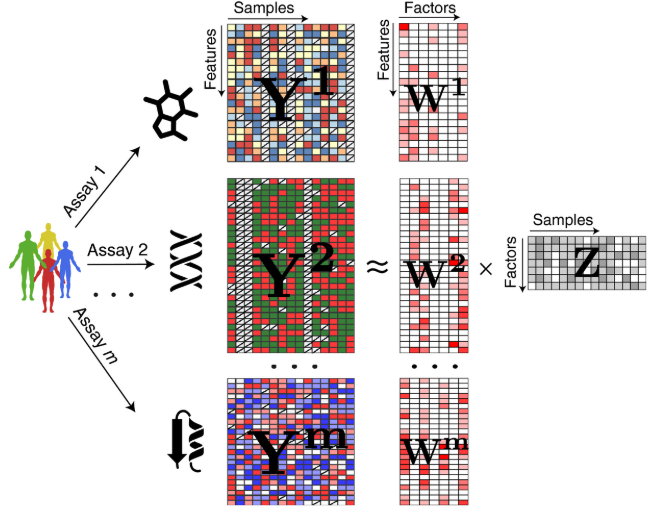
\includegraphics[width=0.75\linewidth]{slides/mofa_schematic.png}
  \caption{Multi-omics factor analysis. Several assays on the same samples give data matrices $\mY^1,\dots,\mY^m$ (drawn as features by samples, the transpose of our convention), each with its own loading matrix $\mW^m$ and a shared factor matrix $\mathbf{Z}$ (our $\mX$). Hatched entries are missing. Reproduced from \citet{argelaguet2018}.}
  \label{fig:mofa_schematic}
\end{figure}

The priors are
\begin{align}
  x_{nk}&\sim\Normal(0,1), \\
  \epsilon^{(m)}_{nd}&\sim\Normal\left(0,1/\tau^{(m)}_d\right), & \tau^{(m)}_d&\sim\Gam(a_0^\tau,b_0^\tau), \\
  w^{(m)}_{dk}&\sim\Normal\left(0,1/\alpha^{(m)}_k\right), & \alpha^{(m)}_k&\sim\Gam(a_0^\alpha,b_0^\alpha).
  \label{eq:mofa_ard}
\end{align}
The prior on the factors is the same as in factor analysis. The noise precision (inverse variance) $\tau^{(m)}_d$ is specific to each feature $d$ of each view, so as in factor analysis some genes can be noisier than others. MOFA also supports non-Gaussian likelihoods for binary data such as mutations and for counts. The new ingredient is the prior on the loadings.

\subsection{Automatic relevance determination}

The prior variance of $w^{(m)}_{dk}$ is $1/\alpha^{(m)}_k$, shared by all features of view $m$ for factor $k$. The $\alpha$s are precisions, and they are learned, with a Gamma prior
\begin{equation}
  \Gam(\alpha\mid a,b)=\frac{b^a}{\Gamma(a)}\alpha^{a-1}e^{-b\alpha}, \qquad \alpha>0,
\end{equation}
which has mean $a/b$. The shape $a$ controls the form of the density (Figure~\ref{fig:gamma_ard}): for $a>1$ it is a unimodal bump on the positive axis, for $a=1$ it is exponential, and for $a<1$ it diverges at zero and has a long tail. MOFA sets $a_0^\alpha=b_0^\alpha=10^{-14}$, so the prior is close to $p(\alpha)\propto1/\alpha$: it is indifferent to the scale of $\alpha$ and allows both very small and very large values.

\begin{figure}[tbp]
  \centering
  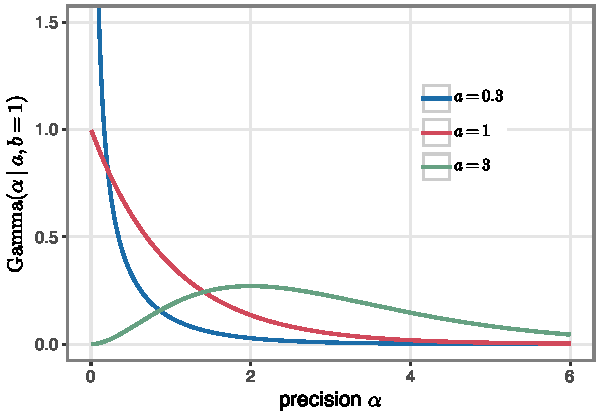
\includegraphics[width=0.5\linewidth]{gamma_ard.pdf}
  \caption{Gamma densities with rate $b=1$ and three shapes $a$. For $a<1$ most of the mass is near zero with a long tail to large values.}
  \label{fig:gamma_ard}
\end{figure}

The effect is to switch factors on and off per view. If $\alpha^{(m)}_k$ is large, the prior variance $1/\alpha^{(m)}_k$ is close to zero, and all loadings of factor $k$ on view $m$ are forced to zero: factor $k$ does not affect that assay. If $\alpha^{(m)}_k$ is small, the prior variance is large and the loadings are free to be large. Learning $\alpha$ from the data therefore determines which factors are relevant to which views, hence the name \emph{automatic relevance determination} (ARD)~\citep{mackay1994,neal1996,bishop1999bpca}. A factor can be active in one view only (for example capturing variation specific to the RNA-seq data), in all views, or in a subset, and the shared factors are often the most interesting. Applied across all factors of a single view, the same prior prunes factors that are not needed, which reduces the sensitivity to the choice of $K$. MOFA additionally places a spike-and-slab prior on each loading, $w^{(m)}_{dk}=\hat w^{(m)}_{dk}s^{(m)}_{dk}$ with $\hat w^{(m)}_{dk}$ following~\eqref{eq:mofa_ard} and $s^{(m)}_{dk}\in\{0,1\}$ Bernoulli, so that each factor affects only some features within an active view. The posterior over all the latent variables and parameters is approximated by variational Bayesian inference, which we cover in a later chapter.

The same factor analysis structure with ARD priors is used by PEER~\citep{stegle2010} to infer hidden confounders in gene expression, which we meet in Chapter 12.

\subsection{Application: chronic lymphocytic leukemia}

\citet{argelaguet2018} applied MOFA to a cohort of 200 patients with chronic lymphocytic leukemia (CLL) profiled with four views: somatic mutations (69 features), RNA-seq (5000 genes), DNA methylation (4248 CpG sites) and \emph{ex vivo} drug response of the patients' cancer cells (310 features, responses to a panel of drugs at several concentrations). Not all patients had every assay (Figure~\ref{fig:mofa_cll}A). The model found 10 factors. Panel B shows the variance explained ($R^2$) by each factor in each view, which reflects the relevance learned through $\alpha^{(m)}_k$: a factor switched off in a view explains no variance there. Factor 1 explains variation in methylation, mutations and drug response, and less in RNA; factor 3 is specific to drug response; factor 4 is specific to gene expression.

The loadings identify the factors (panel D). Factor 1 is driven by the mutation status of the immunoglobulin heavy-chain variable region (IGHV), the main clinical subtype of CLL, and factor 2 by trisomy 12, a gain of a third copy of chromosome 12. A scatter plot of the two factors (panel E) separates patients by these two genetic features. Other factors relate to gene sets (panel F), for example immune response and cellular stress pathways. The general point is that multi-omic data are high-dimensional in each view and heterogeneous across views, and a factor model with view-specific relevance finds a few axes of variation and identifies which are shared across data types.

\begin{figure}[tbp]
  \centering
  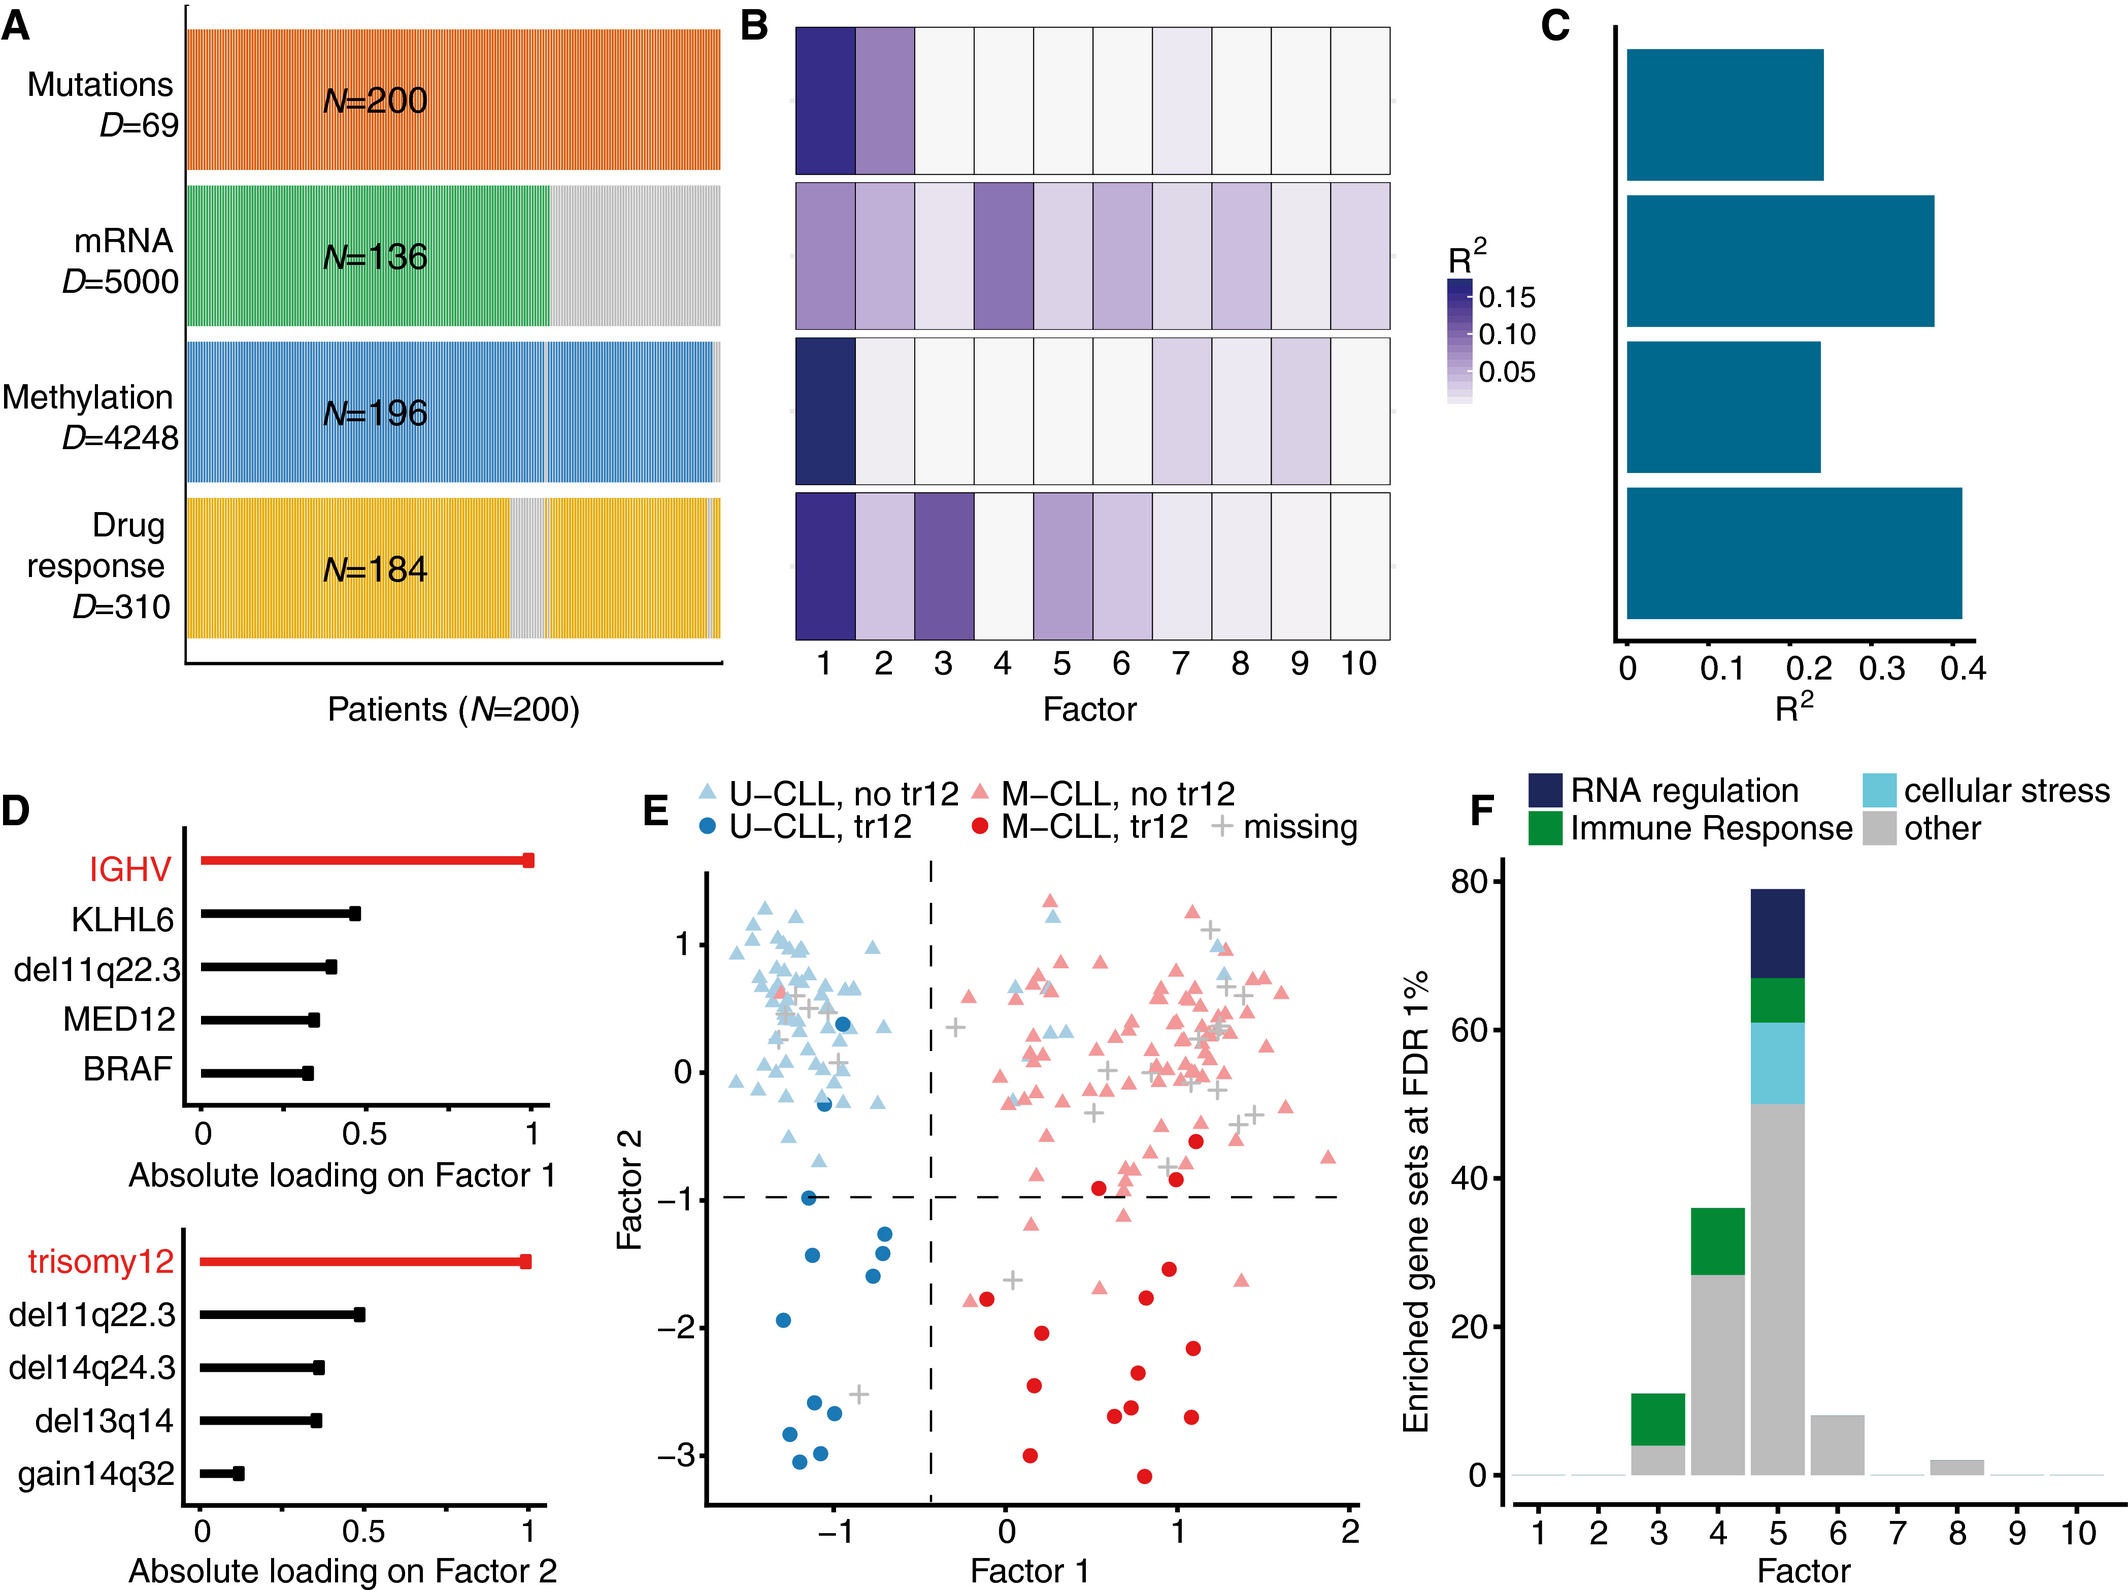
\includegraphics[width=0.95\linewidth]{slides/mofa_cll.png}
  \caption{MOFA applied to chronic lymphocytic leukemia. (A) Four views measured on 200 patients; grey marks missing samples. (B) Variance explained by each factor in each view. (C) Total variance explained per view. (D) Largest absolute loadings of factors 1 and 2 on the mutation view. (E) Patients plotted by factors 1 and 2, coloured by IGHV status (U, unmutated; M, mutated) and trisomy 12. (F) Number of gene sets enriched in the mRNA loadings of each factor. Reproduced from \citet{argelaguet2018}.}
  \label{fig:mofa_cll}
\end{figure}

%======================================================================
\section{Probabilistic principal components analysis}
\label{sec:ppca}
%======================================================================

\subsection{Spherical noise}

Probabilistic PCA~\citep{tipping1999} is factor analysis with one change: the noise covariance is \emph{spherical}, $\mPsi=\sigma^2\mI_P$, a single variance $\sigma^2$ shared by all features,
\begin{equation}
  \vy_n=\mW\vx_n+\veps_n, \qquad \vx_n\sim\Normal(\vzero,\mI_K), \qquad \veps_n\sim\Normal(\vzero,\sigma^2\mI_P),
  \label{eq:ppca}
\end{equation}
so that $\vy_n\sim\Normal(\vzero,\mC)$ with $\mC=\mW\mW^\top+\sigma^2\mI$. Factor analysis allows a separate noise level for each feature; probabilistic PCA assumes they are all equal. Which assumption is better depends on the data. If the features are on different scales or some are much noisier than others, the spherical assumption pushes probabilistic PCA to spend factors explaining the noise of individual features. Figure~\ref{fig:fa_vs_ppca} shows an example with one factor that loads on five features and a sixth feature with large independent noise. Factor analysis recovers the loadings and puts the sixth feature's variance into $\psi_6$; probabilistic PCA with $K=1$ points its single component at the noisy feature, because that is the direction of largest variance. For this reason expression data are usually log-transformed and often standardized before PCA. The advantage of the spherical model is computational: its maximum likelihood estimate has a closed form.

\begin{figure}[tbp]
  \centering
  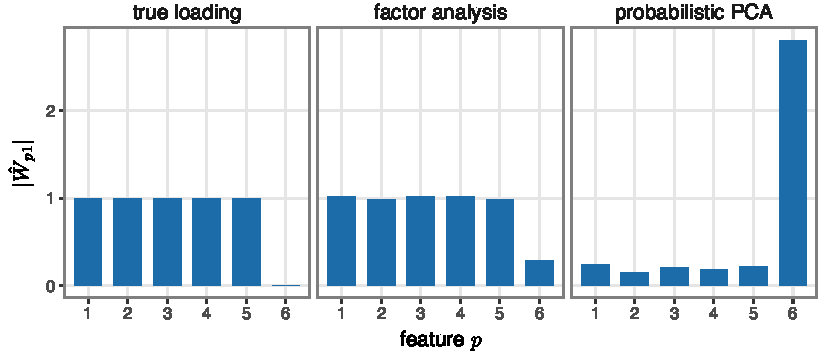
\includegraphics[width=0.85\linewidth]{fa_vs_ppca.pdf}
  \caption{Factor analysis and probabilistic PCA with $K=1$ fitted to $N=500$ simulated points. The true factor loads on features 1--5 (noise variance 0.3 each); feature 6 has no loading and noise variance 9. Factor analysis recovers the loadings; probabilistic PCA puts its component on the noisy feature.}
  \label{fig:fa_vs_ppca}
\end{figure}

\subsection{Maximum likelihood by eigendecomposition}

The log likelihood is~\eqref{eq:fa_loglik_S} with $\mC=\mW\mW^\top+\sigma^2\mI$. The sample covariance $\mS=\frac1N\mY^\top\mY$ is symmetric and positive semi-definite (positive definite if $N>P$ and $\mY$ has full column rank), so it has an eigendecomposition
\begin{equation}
  \mS=\mU\mLambda\mU^\top, \qquad \mU^\top\mU=\mI_P, \qquad \mLambda=\diag(\lambda_1,\dots,\lambda_P),
  \label{eq:eig}
\end{equation}
where $\mU\in\R^{P\times P}$ is orthogonal, its columns $\vu_k$ are the eigenvectors, $\mS\vu_k=\lambda_k\vu_k$, and the eigenvalues are ordered, $\lambda_1\geq\lambda_2\geq\dots\geq\lambda_P\geq0$. Write $\mU_K=\mU[:,1{:}K]$ for the first $K$ columns and $\mLambda_K=\mLambda[1{:}K,1{:}K]$ for the $K$ largest eigenvalues. \citet{tipping1999} showed that the maximum likelihood estimates are
\begin{equation}
  \hat\mW=\mU_K\left(\mLambda_K-\hat\sigma^2\mI_K\right)^{1/2}\mR, \qquad \hat\sigma^2=\frac1{P-K}\sum_{k=K+1}^P\lambda_k,
  \label{eq:ppca_ml}
\end{equation}
where $\mR$ is any $K\times K$ orthogonal matrix, reflecting the rotational non-identifiability, and is usually taken to be $\mI$. The directions of $\hat\mW$ are the $K$ leading eigenvectors of $\mS$. The diagonal matrix $(\mLambda_K-\hat\sigma^2\mI)^{1/2}$ rescales each column $\vu_k$ by $\sqrt{\lambda_k-\hat\sigma^2}$ without changing its direction. The noise variance is the average of the $P-K$ discarded eigenvalues: variance in the directions we do not model as signal is attributed to noise.

To see where~\eqref{eq:ppca_ml} comes from, differentiate~\eqref{eq:fa_loglik_S} with respect to $\mW$. Using $\partial\log|\mC|/\partial\mW=2\mC^{-1}\mW$ and $\partial\tr(\mC^{-1}\mS)/\partial\mW=-2\mC^{-1}\mS\mC^{-1}\mW$ for symmetric $\mC$ and $\mS$, the stationary points satisfy
\begin{equation}
  \mS\mC^{-1}\mW=\mW.
\end{equation}
The push-through identity $(\mW\mW^\top+\sigma^2\mI_P)^{-1}\mW=\mW(\mW^\top\mW+\sigma^2\mI_K)^{-1}$ turns this into $\mS\mW=\mW(\sigma^2\mI+\mW^\top\mW)$. Write the singular value decomposition $\mW=\mL\mD\mR^\top$, with $\mL\in\R^{P\times K}$ having orthonormal columns $\boldsymbol{\ell}_k$, $\mD=\diag(d_1,\dots,d_K)$ and $\mR$ orthogonal. Then $\mW^\top\mW=\mR\mD^2\mR^\top$, and the stationarity condition becomes $\mS\mL\mD\mR^\top=\mL\mD(\sigma^2\mI+\mD^2)\mR^\top$, that is,
\begin{equation}
  \mS\boldsymbol{\ell}_k=(\sigma^2+d_k^2)\,\boldsymbol{\ell}_k \qquad\text{for each }k\text{ with }d_k\neq0.
\end{equation}
Each column direction of $\mW$ is an eigenvector of $\mS$, with eigenvalue $\lambda=\sigma^2+d_k^2$, so $d_k=\sqrt{\lambda-\sigma^2}$. Any $K$ eigenvectors give a stationary point, and \citet{tipping1999} show that the maximum takes those with the $K$ largest eigenvalues; the others are saddle points. Substituting back and maximizing over $\sigma^2$ gives the average of the remaining eigenvalues.

This is unusual: a latent variable model with a likelihood that is not convex in $\mW$ can be fitted exactly, with one call to a standard eigendecomposition routine. The probabilistic formulation also gives a posterior over the factors, the special case of~\eqref{eq:fa_estep} with $\mPsi=\sigma^2\mI$,
\begin{equation}
  \vx_n\mid\vy_n\sim\Normal\left(\mM^{-1}\mW^\top\vy_n,\ \sigma^2\mM^{-1}\right), \qquad \mM=\mW^\top\mW+\sigma^2\mI_K\in\R^{K\times K},
  \label{eq:ppca_post}
\end{equation}
handles missing data through EM, and gives a likelihood with which to compare models.

\subsection{Choosing the number of components}

The eigenvalue $\lambda_k$ is the variance of the data along $\vu_k$, and the \emph{proportion of variance explained} by component $k$ is
\begin{equation}
  \text{PVE}_k=\frac{\lambda_k}{\sum_{k'=1}^P\lambda_{k'}}.
\end{equation}
A plot of the ordered eigenvalues (a \emph{scree plot}, Figure~\ref{fig:eigen}a) typically shows a few large ``signal'' eigenvalues followed by a long tail of small ``noise'' eigenvalues, and a common heuristic is to choose $K$ at the elbow. Two more principled approaches follow from the probabilistic view.

First, the Bayesian treatment of probabilistic PCA allows the marginal likelihood $p(\mY\mid K)$, with $\mW$ integrated out, to be approximated for each $K$~\citep{minka2000}. Choosing the $K$ with the largest approximate marginal likelihood decides how many eigenvectors to treat as signal and how many as noise. Minka's method is implemented in scikit-learn (\texttt{PCA(n\_components="mle")}).

Second, random matrix theory says what the noise eigenvalues should look like. Even if the true covariance is $\sigma^2\mI$, the eigenvalues of the sample covariance are spread out. If the entries of $\mY$ are independent with variance $\sigma^2$, and $N,P\to\infty$ with $P/N\to\gamma\in(0,1]$, the distribution of the eigenvalues of $\mS$ converges to the Marchenko-Pastur law~\citep{marchenko1967}, with density
\begin{equation}
  p(\lambda)=\frac{\sqrt{(\lambda_+-\lambda)(\lambda-\lambda_-)}}{2\pi\sigma^2\gamma\lambda}, \qquad \lambda_-\leq\lambda\leq\lambda_+, \qquad \lambda_\pm=\sigma^2(1\pm\sqrt\gamma)^2.
\end{equation}
Eigenvalues above the upper edge $\lambda_+$ are evidence of signal (Figure~\ref{fig:eigen}). With $N=1000$ samples and $P=200$ features, pure noise of unit variance already produces sample eigenvalues ranging from $0.31$ to $2.09$. Conversely, a factor whose contribution to the variance, $\|\vw_k\|^2$, is below $\sigma^2\sqrt\gamma$ produces no eigenvalue outside the noise bulk and cannot be detected by PCA at all~\citep{baik2005}.

\begin{figure}[tbp]
  \centering
  \begin{subfigure}[b]{0.49\linewidth}
    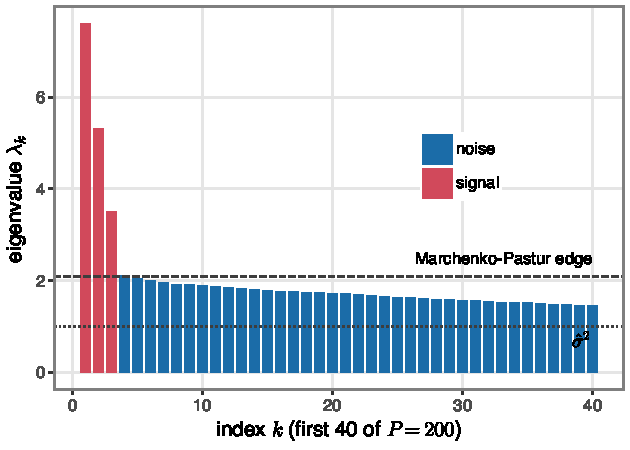
\includegraphics[width=\linewidth]{eigen_scree.pdf}
    \caption{}
  \end{subfigure}\hfill
  \begin{subfigure}[b]{0.49\linewidth}
    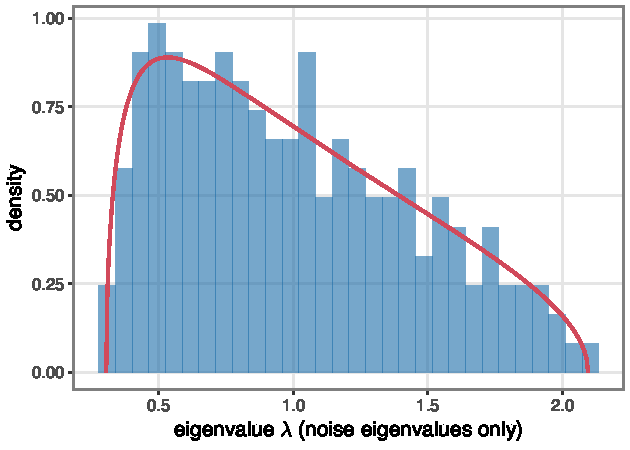
\includegraphics[width=\linewidth]{eigen_mp.pdf}
    \caption{}
  \end{subfigure}
  \caption{Eigenvalues of the sample covariance of simulated data with $N=1000$, $P=200$, $K=3$ factors and noise variance $\sigma^2=1$. (a) The three signal eigenvalues stand above the Marchenko-Pastur upper edge $\lambda_+=(1+\sqrt{0.2})^2\approx2.09$ (dashed); the probabilistic PCA estimate $\hat\sigma^2$, the mean of the remaining eigenvalues, is $0.997$ (dotted). (b) The $197$ noise eigenvalues follow the Marchenko-Pastur density (curve).}
  \label{fig:eigen}
\end{figure}

%======================================================================
\section{Principal components analysis}
\label{sec:pca}
%======================================================================

\subsection{PCA as a limit of probabilistic PCA}

Historically PCA came first~\citep{pearson1901,hotelling1933} and probabilistic PCA was introduced to give it a probabilistic interpretation. Going in the other direction, classical PCA is the limit of probabilistic PCA in which all components are kept, $K\to P$, so that no variance is left for the noise, $\hat\sigma^2\to0$. Then~\eqref{eq:ppca_ml} becomes
\begin{equation}
  \hat\mW=\mU\mLambda^{1/2},
\end{equation}
and $\hat\mW\hat\mW^\top=\mU\mLambda\mU^\top=\mS$ reproduces the sample covariance exactly. As $\sigma^2\to0$ the posterior mean~\eqref{eq:ppca_post} tends to $(\mW^\top\mW)^{-1}\mW^\top\vy_n$, the coordinates of the orthogonal projection of $\vy_n$ onto the column space of $\mW$. In practice one keeps the first $K$ components. The \emph{principal component scores} are the projections $\mY\mU_K\in\R^{N\times K}$, and the rank-$K$ reconstruction $\mY\mU_K\mU_K^\top$ is the best rank-$K$ approximation of $\mY$ in squared error (the Eckart-Young theorem).

\subsection{PCA as the directions of maximal variance}

The classical definition of PCA is that it finds the orthogonal directions along which the data vary most (Figure~\ref{fig:pca_2d}). The variance of the centered data projected onto a unit vector $\vu\in\R^P$ is $\frac1N\sum_n(\vu^\top\vy_n)^2=\vu^\top\mS\vu$. Maximizing this subject to $\vu^\top\vu=1$ with a Lagrange multiplier $\lambda$,
\begin{equation}
  \frac{\partial}{\partial\vu}\left[\vu^\top\mS\vu-\lambda(\vu^\top\vu-1)\right]=2\mS\vu-2\lambda\vu=\vzero
  \quad\Rightarrow\quad \mS\vu=\lambda\vu,
\end{equation}
so $\vu$ is an eigenvector of $\mS$ and the projected variance is $\vu^\top\mS\vu=\lambda$. The maximum is the first eigenvector $\vu_1$, with variance $\lambda_1$. The second principal component maximizes the variance among directions orthogonal to $\vu_1$, which is equivalent to removing the variation along $\vu_1$ and repeating, and gives $\vu_2$; and so on. Eigenvectors of a symmetric matrix are orthogonal, $\vu_i^\top\vu_j=0$ for $i\neq j$.

\begin{figure}[tbp]
  \centering
  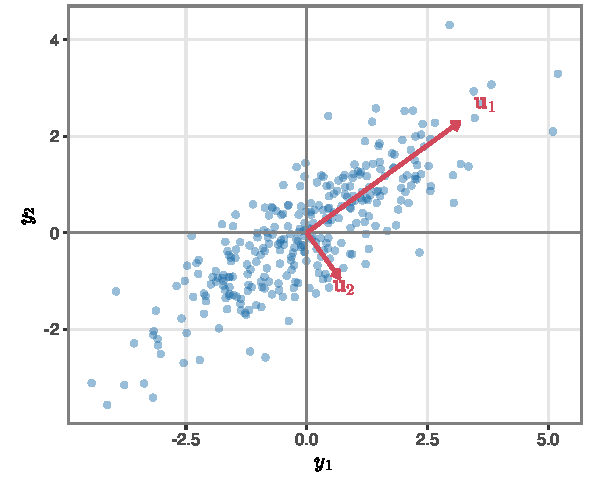
\includegraphics[width=0.5\linewidth]{pca_2d.pdf}
  \caption{PCA of a centered two-dimensional point cloud. The first principal axis $\vu_1$ is the direction of largest variance and $\vu_2$ is orthogonal to it. Each arrow has length $2\sqrt{\lambda_k}$, twice the standard deviation of the data along that axis.}
  \label{fig:pca_2d}
\end{figure}

In practice PCA is computed from the singular value decomposition of the centered data matrix, $\mY=\mA\mD\mB^\top$, without forming $\mS$. Then $\mS=\frac1N\mB\mD^2\mB^\top$, so the eigenvectors are the right singular vectors, $\mU=\mB$, the eigenvalues are $\lambda_k=d_k^2/N$, and the scores are $\mY\mB=\mA\mD$. When only the first few components are needed, truncated or randomized SVD algorithms compute them at a fraction of the cost of the full decomposition.

\subsection{PCA in single-cell analysis}

PCA is a standard first step in most analysis pipelines, and in single-cell RNA-seq it is nearly universal. After normalization and log transformation, the $\sim$20{,}000 genes are filtered to a few thousand highly variable genes, and PCA reduces these to around 30 components. Clustering (Chapter 5), nearest-neighbour graphs and visualizations such as UMAP and t-SNE are then computed in the PC space. This denoises the data, since the discarded components are mostly noise, and makes the downstream computations faster. It is worth considering for any expression analysis whether working with the leading PCs would be better than working with the raw data.

%======================================================================
\section{PCA use case: population structure}
\label{sec:popstruct}
%======================================================================

Two human genomes differ at roughly one position in every thousand, so across the $3\times10^9$ base pairs of the genome a person carries millions of single nucleotide polymorphisms (SNPs) relative to others. Genotyping, by sequencing or with SNP arrays, gives a matrix $\mY\in\{0,1,2\}^{N\times P}$ where $y_{np}$ is the number of copies of the minor allele that individual $n$ carries at SNP $p$, with $P$ in the hundreds of thousands or more. After centering (and usually standardizing) each SNP, PCA of this matrix reveals \emph{population structure}: systematic differences in allele frequencies between groups with different ancestry.

\citet{novembre2008} applied PCA to about 1400 Europeans genotyped at about 200{,}000 SNPs. Plotting the first two PCs, after rotating the axes, reproduces the map of Europe (Figure~\ref{fig:novembre}). Individuals from Spain and Portugal, Italy, France and Switzerland, the British Isles, Scandinavia and south-eastern Europe each occupy the region corresponding to their geography, and barriers to migration such as seas and the Alps appear as gaps. The reason is that for most of the last several thousand years people have mostly had children with partners from nearby. Allele frequencies drift randomly in each place, and limited migration keeps nearby populations similar, so genetic similarity decays with geographic distance. PCA picks up this smooth gradient.

\begin{figure}[tbp]
  \centering
  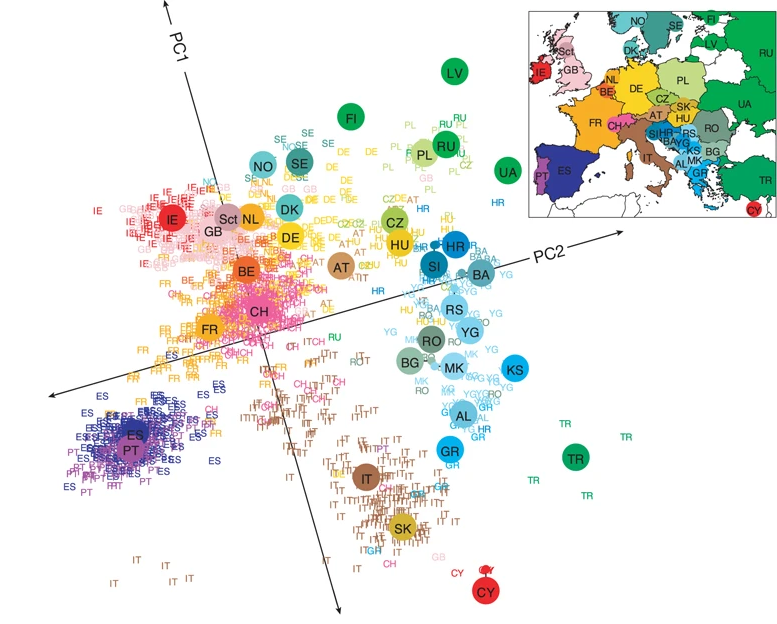
\includegraphics[width=0.75\linewidth]{slides/novembre_pca_europe.png}
  \caption{The first two principal components of genotype data from about 1400 Europeans, coloured by country of origin (labels are country codes; large circles are country medians), with the axes rotated to align with the map (inset). Reproduced from \citet{novembre2008}.}
  \label{fig:novembre}
\end{figure}

Population structure matters because it confounds genetic association studies. A classic example is a study of type 2 diabetes in the Gila River Indian Community in Arizona~\citep{knowler1988}. Individuals carrying the immunoglobulin haplotype $Gm^{3;5,13,14}$ had a much lower prevalence of diabetes at every age (Figure~\ref{fig:knowler}a), suggesting a protective variant. But this haplotype is common in Europeans and rare in Native Americans, and in this community diabetes prevalence rises with the proportion of Native American heritage while the frequency of the haplotype falls (Figure~\ref{fig:knowler}b). The haplotype was a marker of European admixture, and admixture was associated with diabetes risk; when the analysis accounted for heritage, the association largely disappeared. Any variant whose frequency differs between ancestry groups will be associated with any trait that also differs between those groups, for genetic or environmental reasons. A standard correction includes the top genotype PCs as covariates in the association test~\citep{price2006}, which we discuss with genome-wide association studies in Chapter 11.

\begin{figure}[tbp]
  \centering
  \begin{subfigure}[b]{0.38\linewidth}
    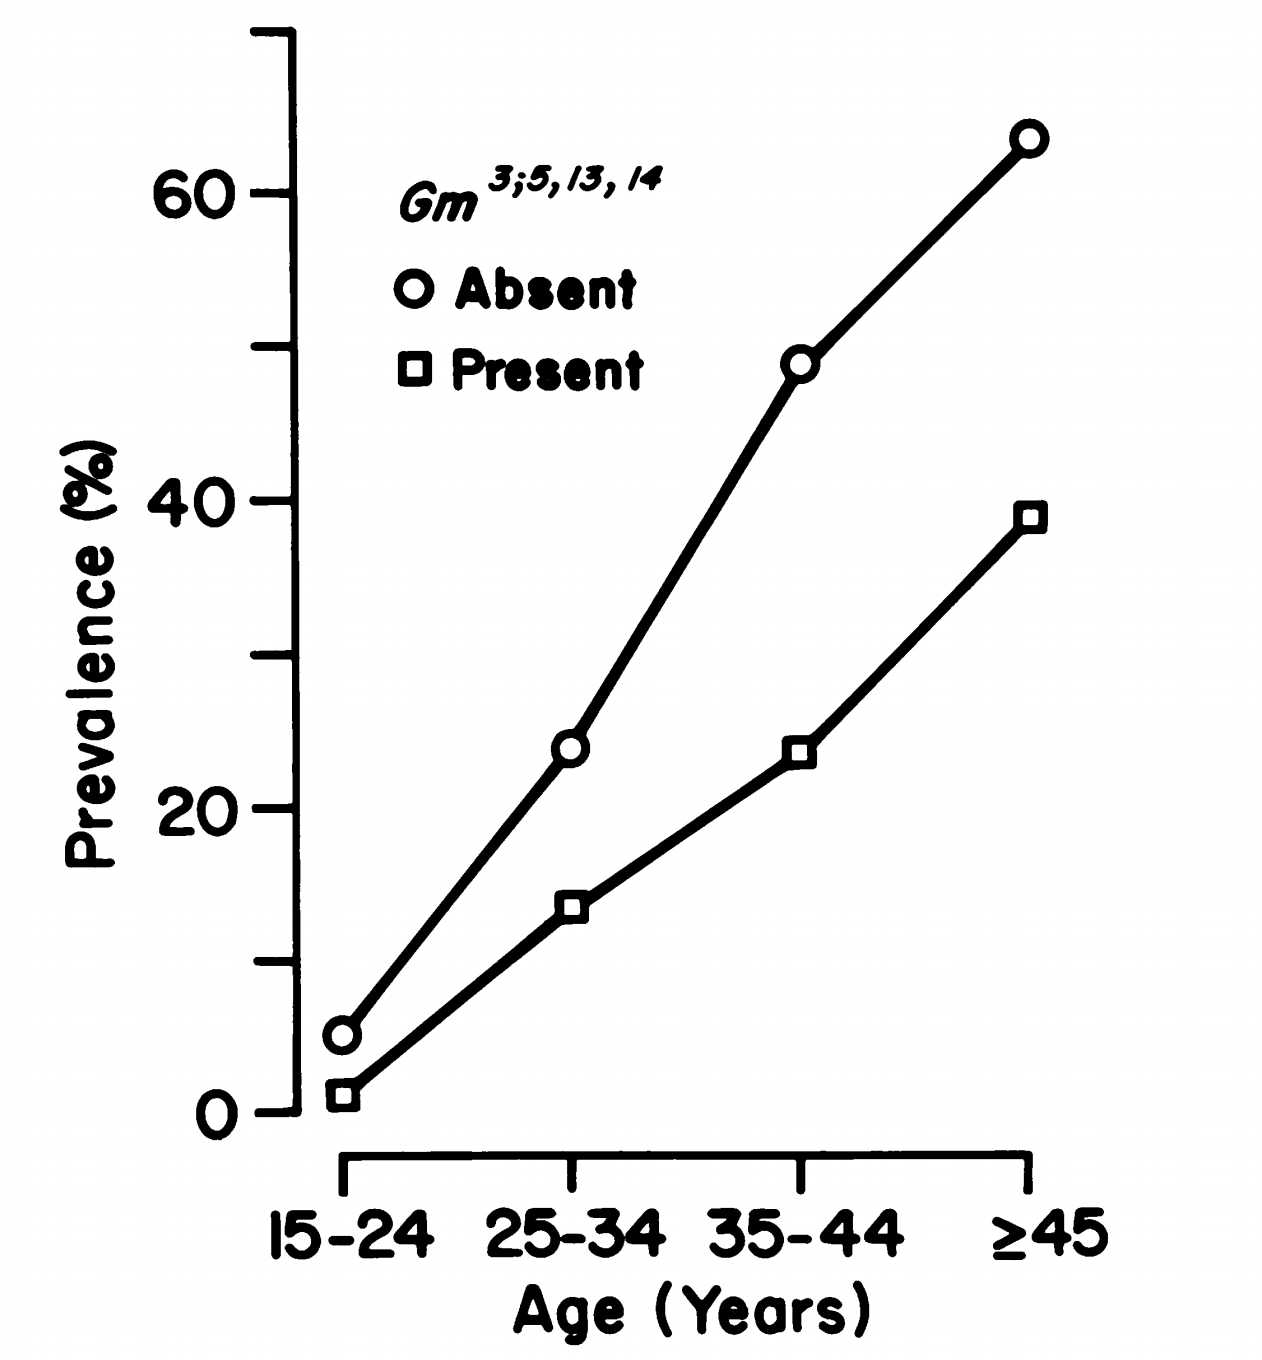
\includegraphics[width=\linewidth]{slides/knowler_fig1.png}
    \caption{}
  \end{subfigure}\hfill
  \begin{subfigure}[b]{0.58\linewidth}
    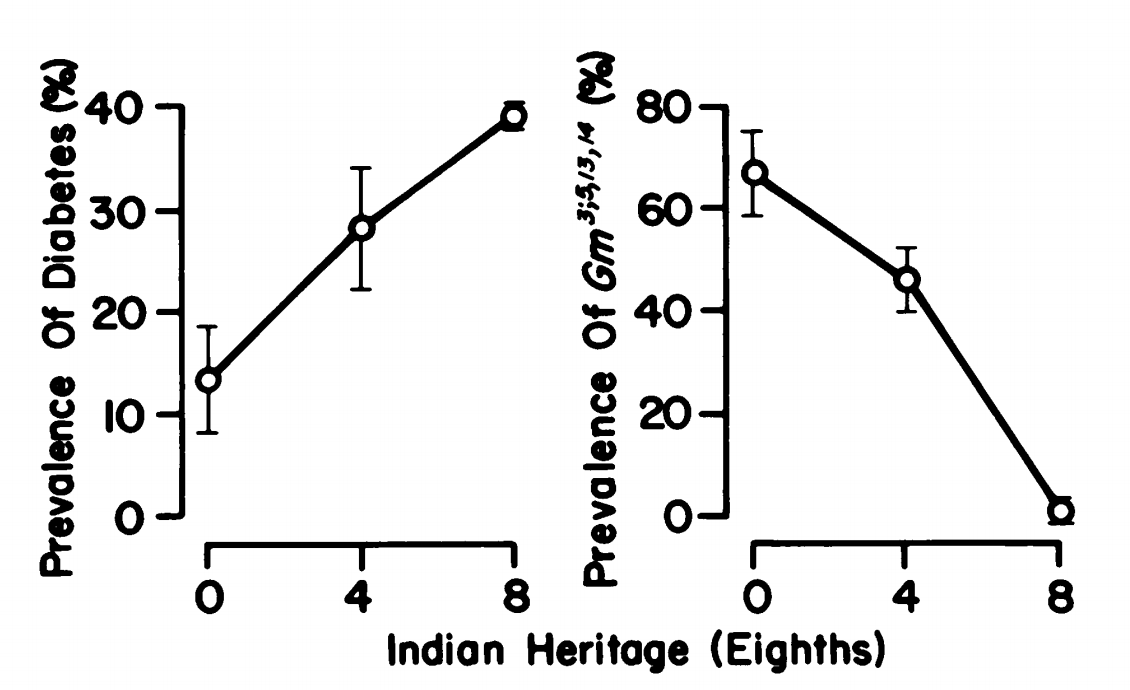
\includegraphics[width=\linewidth]{slides/knowler_fig3.png}
    \caption{}
  \end{subfigure}
  \caption{Confounding by population structure. (a) Prevalence of type 2 diabetes by age among residents of the Gila River Indian Community, by presence of the haplotype $Gm^{3;5,13,14}$. (b) Age-adjusted prevalence ($\pm1$ standard error) of diabetes (left) and of the haplotype (right) by degree of Indian heritage, in eighths. Reproduced from \citet{knowler1988}.}
  \label{fig:knowler}
\end{figure}

%======================================================================
\section{Autoencoders}
\label{sec:ae}
%======================================================================

Recurrent neural networks (Chapter 7) are the deep learning counterpart of hidden Markov models; autoencoders are the deep learning counterpart of matrix factorization. An autoencoder is a neural network trained to reproduce its input. It consists of an \emph{encoder} $f_\phi:\R^P\to\R^K$, which maps a data point $\vy_n$ to a \emph{code} (also called latent representation or embedding) $\vx_n=f_\phi(\vy_n)$, and a \emph{decoder} $g_\theta:\R^K\to\R^P$, which maps the code back to a reconstruction $\hat\vy_n=g_\theta(\vx_n)$ (Figure~\ref{fig:ae}). The parameters $\phi$ and $\theta$ are trained to minimize the reconstruction error,
\begin{equation}
  \min_{\phi,\theta}\sum_{n=1}^N\left\|\vy_n-g_\theta(f_\phi(\vy_n))\right\|^2,
  \label{eq:ae}
\end{equation}
by stochastic gradient descent. Predicting the input from itself is trivial if the network can learn the identity function, so something must stop it from doing so. The simplest constraint is a \emph{bottleneck}, $K\ll P$: the code has fewer dimensions (or, in a convolutional network, fewer channels) than the input, so the network has to find a compressed representation.

\begin{figure}[tbp]
  \centering
  \begin{tikzpicture}[every node/.style={font=\small}, layer/.style={draw, fill=gray!8, minimum width=0.45cm}]
    \node[layer, minimum height=3.2cm] (in) at (0,0) {};
    \node[layer, minimum height=2.3cm] (h1) at (1.8,0) {};
    \node[layer, minimum height=1.1cm, fill=red!15] (code) at (3.6,0) {};
    \node[layer, minimum height=2.3cm] (h2) at (5.4,0) {};
    \node[layer, minimum height=3.2cm] (out) at (7.2,0) {};
    \foreach \a/\b in {in/h1, h1/code, code/h2, h2/out} {
      \draw[gray, dashed] (\a.north east) -- (\b.north west);
      \draw[gray, dashed] (\a.south east) -- (\b.south west);
      \draw[gray, dashed] (\a.north east) -- (\b.south west);
      \draw[gray, dashed] (\a.south east) -- (\b.north west);
    }
    \node[above] at (in.north) {input $\vy_n$};
    \node[above] at (code.north) {code $\vx_n$};
    \node[above] at (out.north) {output $\hat\vy_n$};
    \draw[decorate, decoration={brace, mirror, amplitude=5pt}] (-0.25,-1.8) -- (3.85,-1.8) node[midway, below=6pt] {encoder $f_\phi$};
    \draw[decorate, decoration={brace, mirror, amplitude=5pt}] (3.35,-2.5) -- (7.45,-2.5) node[midway, below=6pt] {decoder $g_\theta$};
    \node[below] at (code.south) {$K\ll P$};
  \end{tikzpicture}
  \caption{An autoencoder. The encoder maps the input $\vy_n\in\R^P$ to a lower-dimensional code $\vx_n\in\R^K$, and the decoder maps the code back to a reconstruction $\hat\vy_n$ of the input. For a denoising autoencoder, the input is a corrupted copy of $\vy_n$ while the reconstruction target is the original.}
  \label{fig:ae}
\end{figure}

\subsection{Linear autoencoders and PCA}

Suppose both encoder and decoder are linear, $\vx_n=\mA\vy_n$ and $\hat\vy_n=\mB\vx_n$ with $\mA\in\R^{K\times P}$ and $\mB\in\R^{P\times K}$. The reconstruction of the whole data matrix is $\hat\mY=\mY\mA^\top\mB^\top$, which has rank at most $K$, and the loss~\eqref{eq:ae} is $\|\mY-\mY\mA^\top\mB^\top\|_F^2$, where $\|\cdot\|_F$ is the Frobenius norm (the square root of the sum of squared entries). By the Eckart-Young theorem no rank-$K$ matrix has smaller squared error than the PCA reconstruction $\mY\mU_K\mU_K^\top$, and the linear autoencoder attains it when $\mB\mA=\mU_K\mU_K^\top$, the orthogonal projection onto the span of the first $K$ principal axes. This holds for $\mB=\mU_K\mG$ and $\mA=\mG^{-1}\mU_K^\top$ with any invertible $\mG\in\R^{K\times K}$, so the decoder spans the PCA subspace but its columns need not be the eigenvectors themselves, the same non-identifiability as in factor analysis. \citet{baldi1989} showed that the loss has no spurious local minima: every local minimum is global and the other stationary points are saddle points. Gradient descent on a linear autoencoder therefore finds the PCA subspace (Figure~\ref{fig:linear_ae}).

\begin{figure}[tbp]
  \centering
  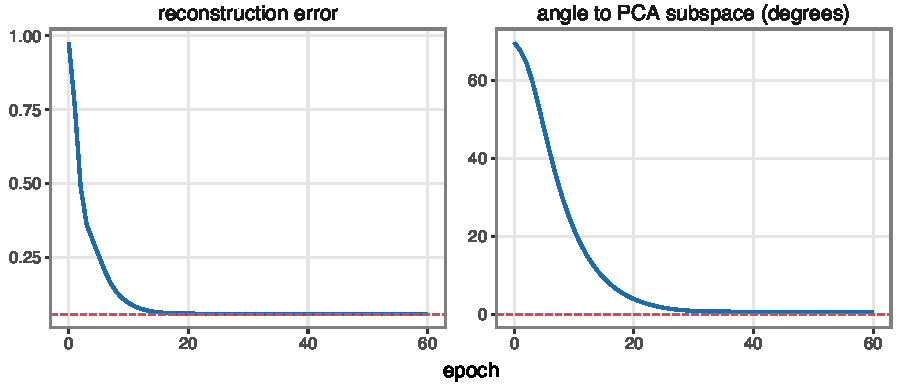
\includegraphics[width=0.9\linewidth]{linear_ae.pdf}
  \caption{A linear autoencoder with $K=3$ trained by minibatch gradient descent on simulated data ($N=2000$, $P=20$, three true factors). Left, the mean squared reconstruction error approaches that of the rank-3 PCA reconstruction (dashed). Right, the largest principal angle between the column space of the decoder $\mB$ and the span of the first three principal axes goes to zero.}
  \label{fig:linear_ae}
\end{figure}

This equivalence has two uses. It gives intuition for what autoencoders do: a nonlinear autoencoder performs a nonlinear analogue of PCA, learning a low-dimensional manifold rather than a subspace~\citep{hinton2006}. And it is a practical way to fit PCA on very large data, since minibatch gradient descent never needs the whole matrix in memory. It also explains the name \emph{latent space} used for autoencoder codes: in the linear case the code is exactly the latent variable $\vx_n$ of probabilistic PCA.

\subsection{Variants}

\begin{itemize}
  \item \emph{Denoising autoencoders}~\citep{vincent2008} corrupt the input, for example by adding noise or setting random entries to zero, and train the network to reconstruct the uncorrupted original, $\min\sum_n\|\vy_n-g_\theta(f_\phi(\tilde\vy_n))\|^2$ with $\tilde\vy_n$ the corrupted copy. The idea is the same as masked language modelling (Chapter 7). Diffusion models~\citep{ho2020} develop the idea formally: they train a denoiser at many known noise levels and use it to generate data.
  \item \emph{Tied} (coupled) autoencoders share parameters between encoder and decoder; in the linear case $\mA=\mB^\top$, as in PCA, where the scores are $\mY\mU_K$ and the reconstruction is $\mY\mU_K\mU_K^\top$. This halves the number of parameters and can help a little.
  \item \emph{Convolutional autoencoders} use convolutions in the encoder and transposed convolutions in the decoder, the operation used by the deconvolutional networks of Chapter 4.
  \item \emph{Variational autoencoders}~\citep{kingma2014} treat the decoder as the generative model $p(\vy_n\mid\vx_n)$ of a latent variable model and the encoder as an \emph{inference network} that outputs an approximate posterior $q(\vx_n\mid\vy_n)$. They are an instance of variational inference, which we cover in a later chapter.
\end{itemize}

%======================================================================
\section{Independent components analysis}
\label{sec:ica}
%======================================================================

\subsection{Heavy-tailed factors}

Independent components analysis keeps the linear model $\vy_n=\mW\vx_n+\veps_n$ but replaces the Gaussian prior on the factors by a heavy-tailed one, with independent components,
\begin{equation}
  p(\vx_n)=\prod_{k=1}^Kp(x_{nk}),
\end{equation}
where $p(x)$ is, for example, a Student-$t$, Laplace ($p(x)\propto e^{-\lambda|x|}$) or Cauchy density. Compared with a Gaussian of the same variance, a heavy-tailed density has more mass near zero and in the tails and less at intermediate values (Figure~\ref{fig:ica}a). This is the same distinction as between the Gaussian and sparse priors on regression coefficients in Chapter 1. Draws from such a prior are \emph{sparse}: for a given data point, most factors are near zero and a few are large.

Figure~\ref{fig:ica}b shows what this does to the data. With Gaussian factors the data form an elliptical cloud. With heavy-tailed factors most points are near the origin, and the rest lie along the directions of individual columns $\vw_k$, because it is rare for two factors to be large at once. The cloud has ``arms'' along the true directions.

\begin{figure}[tbp]
  \centering
  \begin{subfigure}[b]{\linewidth}
    \centering
    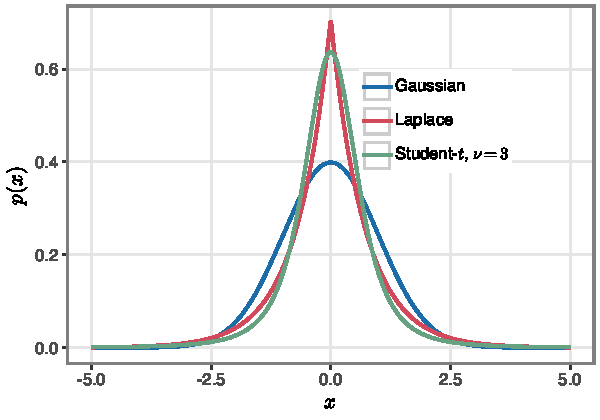
\includegraphics[width=0.5\linewidth]{ica_priors.pdf}
    \caption{}
  \end{subfigure}\\[0.5em]
  \begin{subfigure}[b]{\linewidth}
    \centering
    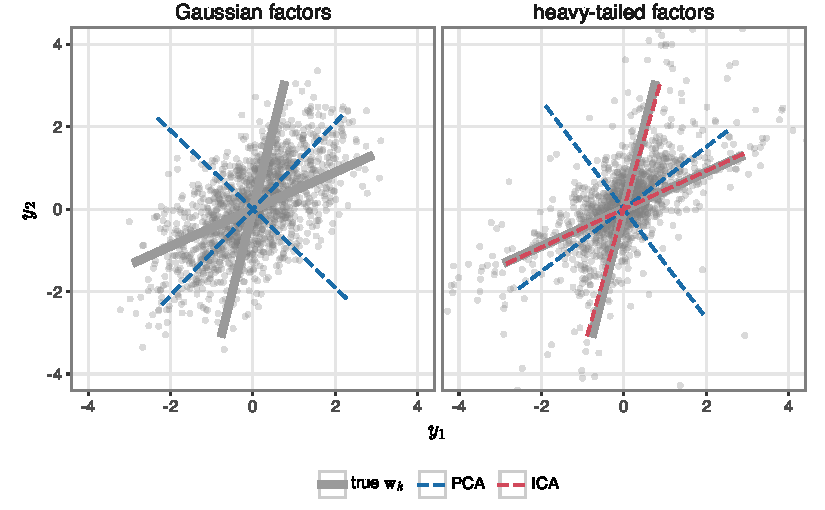
\includegraphics[width=0.85\linewidth]{ica_scatter.pdf}
    \caption{}
  \end{subfigure}
  \caption{Independent components analysis. (a) Gaussian, Laplace and Student-$t$ densities with unit variance; the heavy-tailed densities have more mass near zero and in the tails. (b) Data $\vy_n=\mW\vx_n$ (plus small noise) generated with the same non-orthogonal $\mW$ from Gaussian factors (left) and Student-$t$ factors with 1.5 degrees of freedom (right). Grey lines are the true directions $\vw_1,\vw_2$, blue dashed lines the principal axes, which are orthogonal. With heavy-tailed factors, FastICA (red dashed) recovers the true directions; with Gaussian factors no method can, because the distribution is rotation invariant.}
  \label{fig:ica}
\end{figure}

\subsection{Identifiability}

The heavy-tailed prior resolves the rotational non-identifiability of factor analysis. If $\vx_n\sim\Normal(\vzero,\mI)$ then $\mR^\top\vx_n$ has the same distribution for any orthogonal $\mR$, so $\mW$ and $\mW\mR$ fit equally well. With independent non-Gaussian components, a rotation mixes the components and produces a vector whose entries are no longer independent and whose marginals are closer to Gaussian, by the central limit theorem. The directions $\vw_k$ are then identifiable up to permutation and scaling, provided at most one component is Gaussian~\citep{comon1994}. In Figure~\ref{fig:ica}b the principal axes are orthogonal and do not match the true directions in either panel, while ICA recovers them when the factors are heavy tailed.

Why would biological factors be sparse? Many processes are close to on or off. An immune response is inactive in most cells most of the time and active, to a varying degree, in a few; a cell either is a neuron or is not. A Gaussian factor says every sample is always a little active in every program, which fits such variation poorly.

\subsection{FastICA}

Fitting ICA by maximum likelihood is awkward because the priors are non-standard. The most widely used algorithm is FastICA~\citep{hyvarinen1999,hyvarinen2000}, which is derived from maximizing the non-Gaussianity of the recovered components and works in the noiseless setting with $K=P$ or after reducing to $K$ dimensions by PCA. The data are first \emph{whitened}, $\vz_n=\mLambda_K^{-1/2}\mU_K^\top\vy_n$, so that $\frac1N\sum_n\vz_n\vz_n^\top=\mI_K$. After whitening the remaining unknown is a rotation. For one component, FastICA seeks a unit vector $\vw\in\R^K$ such that $\vw^\top\vz_n$ is as non-Gaussian as possible, using the fixed-point iteration
\begin{equation}
  \vw\leftarrow\frac1N\sum_n\vz_n\,g(\vw^\top\vz_n)-\left[\frac1N\sum_ng'(\vw^\top\vz_n)\right]\vw, \qquad \vw\leftarrow\vw/\|\vw\|,
\end{equation}
where $g$ is a non-linearity such as $g(u)=\tanh(u)$. A fixed-point algorithm repeatedly applies an update until the estimate stops changing; this one is a Newton step and converges quickly. Several components are found together by applying the update to each row of a matrix and re-orthogonalizing the rows after each step. FastICA is fast and has no tuning parameters beyond $K$ and $g$, so it is a reasonable alternative to PCA when sparse, on-off factors are plausible.

%======================================================================
\section{Non-negative matrix factorization}
\label{sec:nmf}
%======================================================================

\subsection{The model}

Many genomic data are non-negative: read counts, normalized expression, mutation counts. Non-negative matrix factorization~\citep{lee1999} approximates a non-negative $\mY\in\R_{\geq0}^{N\times P}$ by $\mX\mW^\top$ with both factors constrained to be non-negative,
\begin{equation}
  \min_{\mX\geq0,\ \mW\geq0}\ \left\|\mY-\mX\mW^\top\right\|_F^2,
  \label{eq:nmf}
\end{equation}
where $\mX\in\R_{\geq0}^{N\times K}$, $\mW\in\R_{\geq0}^{P\times K}$ and the inequalities hold element-wise. Replacing the squared error by the Kullback-Leibler divergence gives the maximum likelihood estimate under a Poisson model for counts, $y_{np}\sim\text{Poisson}(\sum_kx_{nk}w_{pk})$.

Because nothing can be subtracted, each data point has to be built up by adding non-negative parts. NMF therefore tends to give a \emph{parts-based} representation~\citep{lee1999}: each column of $\mW$ is a set of genes that are expressed together (a gene program or ``metagene''~\citep{brunet2004}), and each sample's expression is a non-negative mixture of programs. In PCA, by contrast, loadings and scores have both signs, and a sample can be described as one program minus another, which is harder to interpret. Figure~\ref{fig:nmf} shows simulated data generated from three overlapping non-negative gene programs: NMF recovers the programs, while the principal axes are orthogonal combinations with mixed signs. The non-negativity constraint also removes most of the rotational freedom of factor analysis, since a rotation of non-negative factors generally produces negative entries. A prominent genomic application is the discovery of mutational signatures, the characteristic patterns of somatic mutations left by different mutational processes in cancer genomes~\citep{alexandrov2013}.

\begin{figure}[tbp]
  \centering
  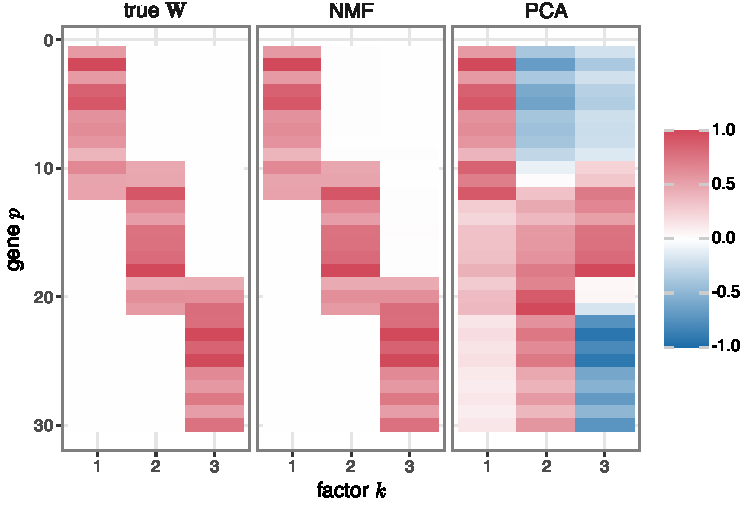
\includegraphics[width=0.75\linewidth]{nmf_vs_pca.pdf}
  \caption{Loadings for simulated non-negative data generated from three overlapping gene programs ($N=300$ samples, $P=30$ genes). Each column is scaled to a maximum absolute value of 1. NMF recovers the programs; PCA loadings mix the programs and have both signs.}
  \label{fig:nmf}
\end{figure}

\subsection{Multiplicative updates}

Problem~\eqref{eq:nmf} is not jointly convex in $\mX$ and $\mW$ but is convex in each given the other. \citet{lee2001} proposed alternating multiplicative updates. The gradient of the objective with respect to $\mX$ is $-2(\mY\mW-\mX\mW^\top\mW)$. A gradient step with an element-wise step size $\eta_{nk}=x_{nk}/(2[\mX\mW^\top\mW]_{nk})$ gives
\begin{equation}
  x_{nk}\leftarrow x_{nk}+\frac{x_{nk}}{[\mX\mW^\top\mW]_{nk}}\left([\mY\mW]_{nk}-[\mX\mW^\top\mW]_{nk}\right)
  = x_{nk}\frac{[\mY\mW]_{nk}}{[\mX\mW^\top\mW]_{nk}},
\end{equation}
and by symmetry
\begin{equation}
  w_{pk}\leftarrow w_{pk}\frac{[\mY^\top\mX]_{pk}}{[\mW\mX^\top\mX]_{pk}}.
\end{equation}
All quantities in the ratios are non-negative, so the updates keep $\mX$ and $\mW$ non-negative without any projection, and \citet{lee2001} showed that the objective never increases. Faster alternatives solve each half as a non-negative least squares problem. As with $K$-means (Chapter 5), the solution depends on the initialization.

\subsection{Integrating single-cell datasets: LIGER}

Single-cell datasets of the same tissue measured with different technologies, in different laboratories or on different days, differ systematically even when they contain the same cell types. These \emph{batch effects} can dominate the variation: a low-dimensional embedding of two datasets combined often separates them by dataset rather than by cell type. LIGER (linked inference of genomic experimental relationships)~\citep{welch2019} integrates datasets with a joint NMF. It is in a sense the opposite of MOFA. In MOFA the samples are shared and each view has its own features; in LIGER each dataset $i=1,\dots,I$ has its own cells $\mY_i\in\R_{\geq0}^{N_i\times P}$ but all datasets measure the same $P$ genes. LIGER therefore uses dataset-specific factors and loadings that are shared up to a dataset-specific perturbation,
\begin{equation}
  \mY_i\approx\mX_i(\mW+\mV_i)^\top,
\end{equation}
with $\mX_i\in\R_{\geq0}^{N_i\times K}$, a shared $\mW\in\R_{\geq0}^{P\times K}$ and dataset-specific $\mV_i\in\R_{\geq0}^{P\times K}$ (Figure~\ref{fig:liger_schematic}). The objective is
\begin{equation}
  \min_{\mX_i,\mV_i,\mW\geq0}\ \sum_{i=1}^I\left\|\mY_i-\mX_i(\mW+\mV_i)^\top\right\|_F^2+\lambda\sum_{i=1}^I\left\|\mX_i\mV_i^\top\right\|_F^2.
  \label{eq:liger}
\end{equation}
Expanding the first term, the residual is $\mY_i-\mX_i\mW^\top-\mX_i\mV_i^\top$. The penalty shrinks the dataset-specific contribution $\mX_i\mV_i^\top$, so the model explains as much of the data as it can with the shared loadings and uses $\mV_i$ only for what the shared part cannot capture. Equivalently, each dataset has its own loadings $\mW_i=\mW+\mV_i$, and the penalty keeps them close to one another; $\lambda$ sets how close. The problem is solved by alternating non-negative least squares.

\begin{figure}[tbp]
  \centering
  \begin{tikzpicture}[every node/.style={font=\small}]
    \foreach \i/\c/\h/\y in {1/blue/1.9/0, 2/red/1.4/-2.6} {
      \draw[fill=\c!25] (0,\y) rectangle (2.4,\y-\h);
      \node at (1.2,\y-\h/2) {$\mY_\i$};
      \node[left] at (0,\y-\h/2) {$N_\i$};
      \node at (2.8,\y-\h/2) {$\approx$};
      \draw[fill=\c!25] (3.2,\y) rectangle (3.8,\y-\h);
      \node at (3.5,\y-\h/2) {$\mX_\i$};
      \node at (4.15,\y-\h/2) {$\times$};
      \node at (4.5,\y-\h/2) {\Large(};
      \draw[fill=black!70] (4.8,\y-\h/2+0.6) rectangle (7.2,\y-\h/2+0.05);
      \node[white] at (6.0,\y-\h/2+0.33) {shared $\mW^\top$};
      \node at (6.0,\y-\h/2-0.12) {$+$};
      \draw[fill=\c!25] (4.8,\y-\h/2-0.3) rectangle (7.2,\y-\h/2-0.85);
      \node at (6.0,\y-\h/2-0.57) {specific $\mV_\i^\top$};
      \node at (7.5,\y-\h/2) {\Large)};
    }
    \node[above] at (1.2,0) {$P$ genes};
    \node[above] at (3.5,0) {$K$};
    \node[above] at (6.0,-0.2) {$P$ genes};
  \end{tikzpicture}
  \caption{LIGER integrates datasets that measure the same $P$ genes in different cells. Each dataset $i$ has its own factors $\mX_i$ and loadings $\mW+\mV_i$, the sum of loadings shared by all datasets and a dataset-specific part. After \citet{welch2019}.}
  \label{fig:liger_schematic}
\end{figure}

After fitting, the factors $\mX_i$ of all datasets live in a common space and serve as the representation of each cell; LIGER further normalizes them across datasets before clustering. Figure~\ref{fig:liger_tsne} shows peripheral blood mononuclear cells profiled with two technologies, Seq-Well and 10x Genomics. In a t-SNE embedding of the LIGER factors (t-SNE and UMAP are nonlinear two-dimensional embeddings discussed in Chapter 5), cells from the two technologies overlap, and the clusters correspond to cell types such as T cells, NK cells, B cells and monocytes, rather than to technology. Integration of this kind works when there is shared biological structure for the model to align; it cannot recover cell types that are present in only one dataset and resemble nothing in the others.

\begin{figure}[tbp]
  \centering
  \begin{subfigure}[b]{0.36\linewidth}
    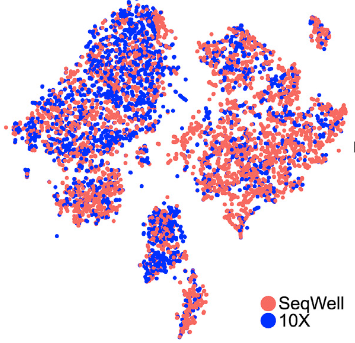
\includegraphics[width=\linewidth]{slides/liger_tsne_technology.png}
    \caption{}
  \end{subfigure}\hfill
  \begin{subfigure}[b]{0.6\linewidth}
    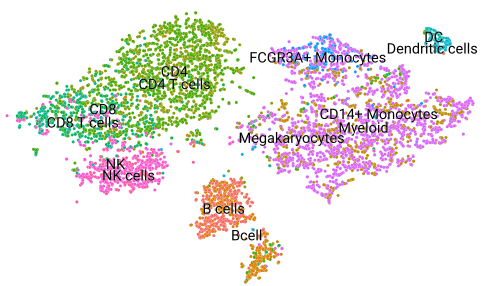
\includegraphics[width=\linewidth]{slides/liger_tsne_celltype.png}
    \caption{}
  \end{subfigure}
  \caption{t-SNE embedding of LIGER factors for peripheral blood cells profiled with Seq-Well and 10x technologies, coloured by (a) technology and (b) cell type label from the original studies. Reproduced from \citet{welch2019}.}
  \label{fig:liger_tsne}
\end{figure}

%======================================================================
\section{Cell type deconvolution of bulk expression}
\label{sec:deconv}
%======================================================================

\subsection{Motivation}

Large patient cohorts, such as The Cancer Genome Atlas, mostly have \emph{bulk} RNA-seq, which measures the summed expression of all cells in a tissue sample. A tumour sample contains cancer cells and also stromal and immune cells, and the immune cells, which may be attacking the tumour or be suppressed by it, are of great clinical interest. \emph{Cell type deconvolution} estimates the proportions of cell types in each bulk sample from its expression profile and a reference expression profile for each cell type. CIBERSORT~\citep{newman2015} made the approach popular and started a large subfield. Its reference profiles came from bulk RNA of experimentally purified cell populations; modern methods typically build them from single-cell RNA-seq, which allows the resolution of the cell types (for example all T cells, or cytotoxic and helper T cells separately) to be chosen \emph{in silico} after the data are generated, rather than fixed by the sorting strategy used to purify the cells.

\begin{figure}[tbp]
  \centering
  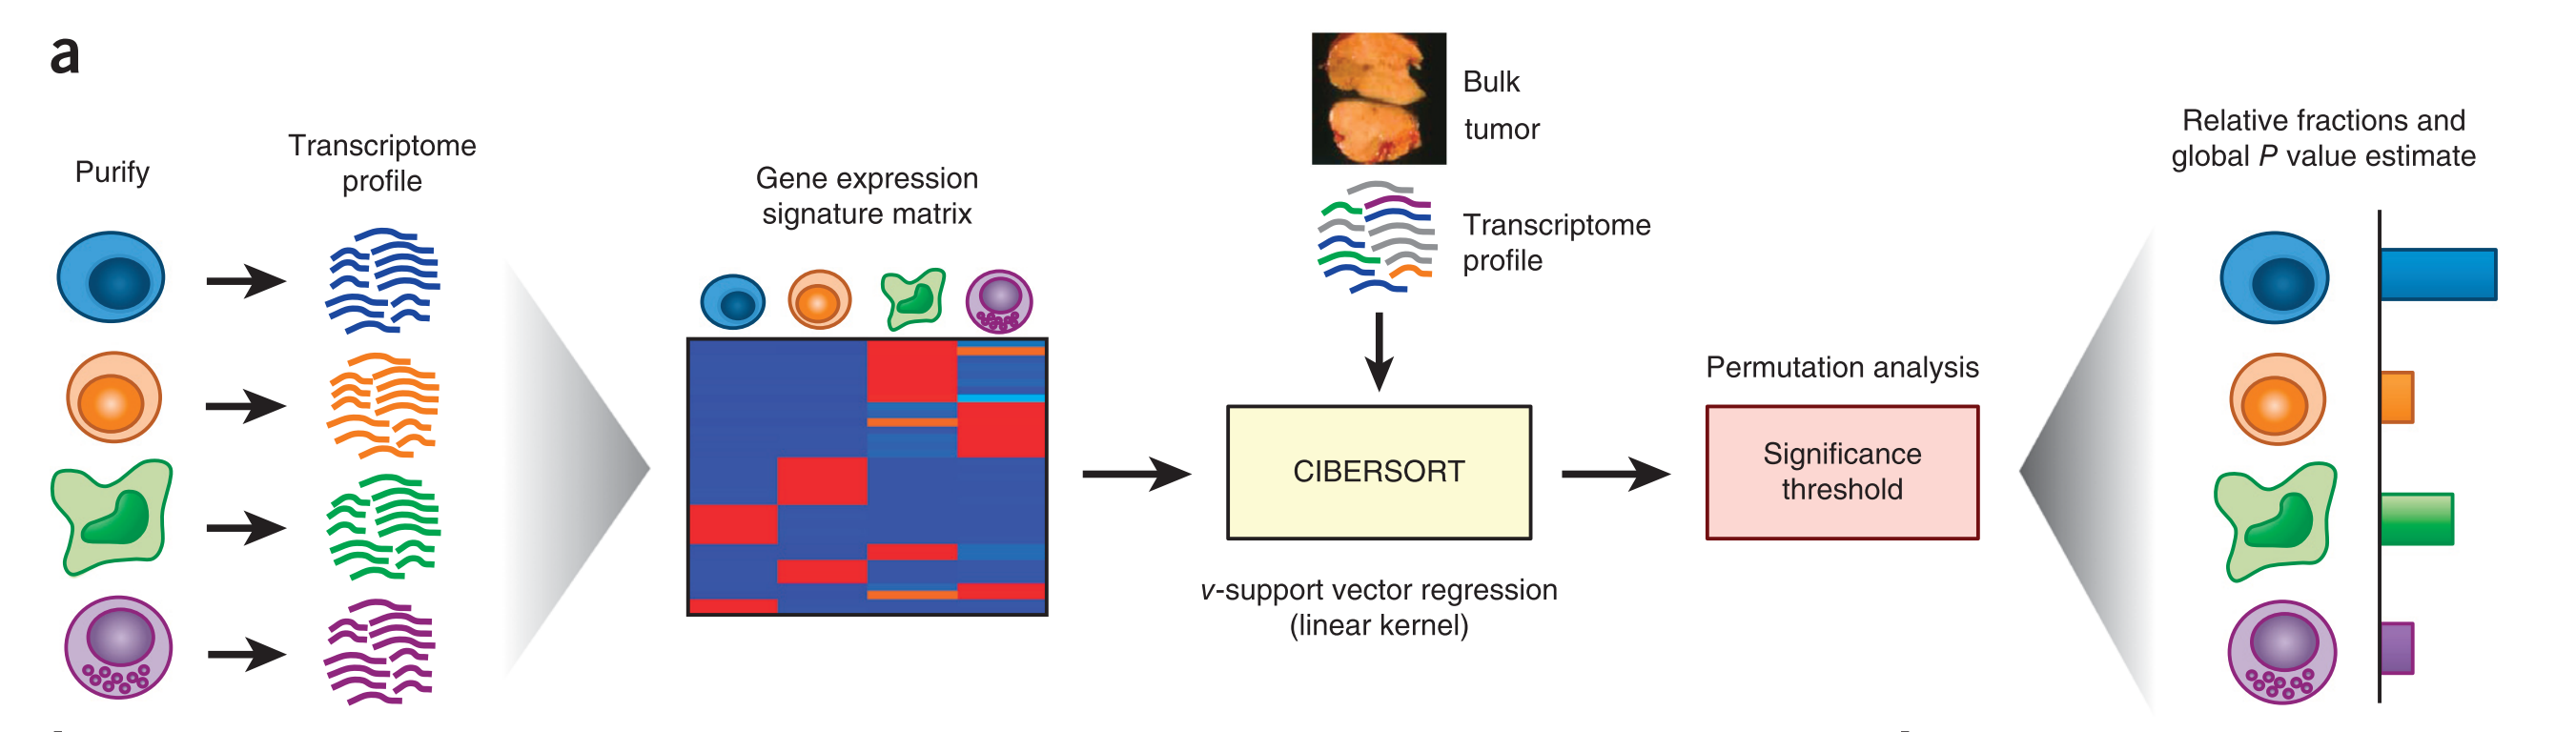
\includegraphics[width=\linewidth]{slides/cibersort_schematic.png}
  \caption{CIBERSORT. Expression profiles of purified cell types form a signature matrix (our $\mW$). The transcriptome of a bulk tumour sample is deconvolved by $\nu$-support vector regression with a linear kernel, giving the relative fractions of the cell types and a $P$ value from a permutation test. Reproduced from \citet{newman2015}.}
  \label{fig:cibersort}
\end{figure}

\subsection{Deconvolution as regression}

Deconvolution has the form of a matrix factorization in which one factor is known. Let $\mY\in\R^{N\times P}$ hold the bulk expression of $P$ genes in $N$ samples, and let $\mW\in\R^{P\times K}$ be the \emph{signature matrix}, with $w_{pk}$ the expression of gene $p$ in cell type $k$ and $K$ the number of cell types. Then
\begin{equation}
  \mY=\mX\mW^\top+\mE, \qquad \vy_n=\mW\vx_n+\veps_n,
\end{equation}
where $x_{nk}$ is the abundance of cell type $k$ in sample $n$, the quantity we want. Since $\mW$ is known, estimating $\vx_n$ is a linear regression for each sample separately, in which the ``data points'' are the $P$ genes and the ``covariates'' are the $K$ columns of $\mW$. Any feature with cell-type-specific signal can be used, for example chromatin accessibility instead of expression.

What makes the problem unusual is the residual $\veps_n$. The signature matrix covers immune and stromal cell types, but a tumour sample also contains cancer cells, whose expression is not in $\mW$ and differs between patients. Their contribution ends up in $\veps_n$, and it is large for the genes the cancer cells express highly. A squared-error loss lets a few genes with large residuals dominate the fit. CIBERSORT instead uses support vector regression, whose loss grows only linearly for large residuals.

\subsection{Support vector regression}

The $\epsilon$-insensitive loss of a residual $r$ is
\begin{equation}
  \ell_\epsilon(r)=\max(0,|r|-\epsilon),
\end{equation}
which is zero inside a ``tube'' $|r|\leq\epsilon$ and grows linearly outside it (Figure~\ref{fig:svr}a). Support vector regression (SVR) for sample $n$ minimizes
\begin{equation}
  \min_{\vx_n,b}\ \frac12\|\vx_n\|^2+C\sum_{p=1}^P\ell_\epsilon\left(y_{pn}-\vw_p^\top\vx_n-b\right),
  \label{eq:svr}
\end{equation}
where $\vw_p^\top$ is row $p$ of $\mW$, $b$ is an intercept and $C>0$ balances the loss against the L2 penalty on $\vx_n$. The lecture slides write the same objective summed over all samples with $C=1$ and no intercept. Compared with squared error, a residual twice as large costs twice as much rather than four times as much, so the fit tolerates a few genes with large errors, such as those dominated by cancer-cell expression (Figure~\ref{fig:svr}b). The absolute loss is the negative log likelihood of Laplace noise, so SVR with $\epsilon=0$ is ridge-penalized least absolute deviation regression, the robust counterpart of ridge regression.

\begin{figure}[tbp]
  \centering
  \begin{subfigure}[b]{0.44\linewidth}
    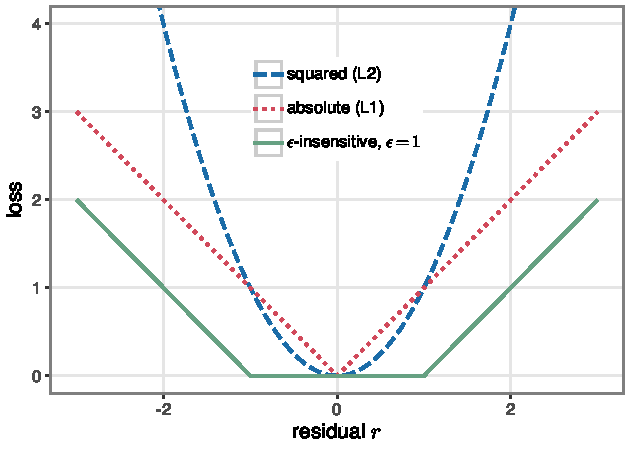
\includegraphics[width=\linewidth]{svr_losses.pdf}
    \caption{}
  \end{subfigure}\hfill
  \begin{subfigure}[b]{0.52\linewidth}
    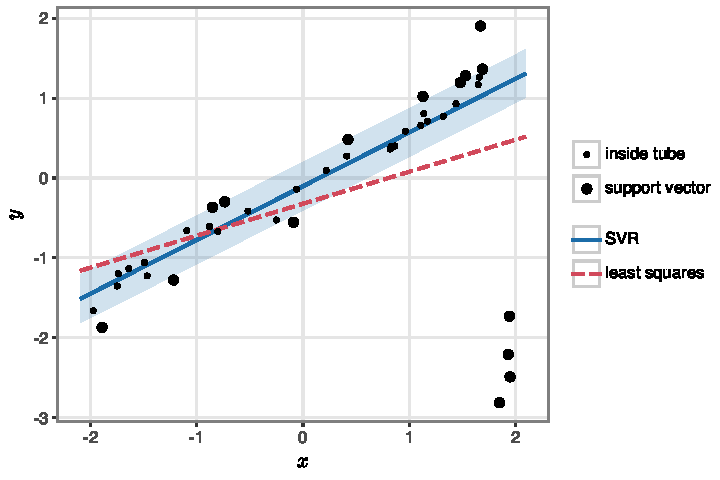
\includegraphics[width=\linewidth]{svr_fit.pdf}
    \caption{}
  \end{subfigure}
  \caption{Support vector regression. (a) Squared, absolute and $\epsilon$-insensitive losses as functions of the residual. (b) Linear SVR with $\epsilon=0.3$ (blue line and tube) and least squares (red dashed) fitted to simulated data with true slope $0.8$ and four outliers at the right. The least-squares slope is pulled down to $0.40$; the SVR slope is $0.67$. Large points are support vectors, on or outside the tube; the fit depends only on them.}
  \label{fig:svr}
\end{figure}

The solution of~\eqref{eq:svr} can be written, through its dual problem, as $\vx_n=\sum_p(a_p-a_p^*)\vw_p$ with dual variables $a_p,a_p^*\in[0,C]$ that are non-zero only for genes whose residual is on or outside the tube. These genes are the \emph{support vectors}. Genes fitted to within $\epsilon$ do not affect the solution at all. The lasso is sparse in the coefficients; SVR is sparse in the data points.

Choosing $\epsilon$ requires knowing the scale of the residuals. $\nu$-SVR~\citep{scholkopf2000} replaces $\epsilon$ by a parameter $\nu\in(0,1]$ and estimates $\epsilon\geq0$ as part of the optimization,
\begin{equation}
  \min_{\vx_n,b,\epsilon\geq0}\ \frac12\|\vx_n\|^2+C\left(\nu\epsilon+\frac1P\sum_{p=1}^P\ell_\epsilon\left(y_{pn}-\vw_p^\top\vx_n-b\right)\right).
\end{equation}
\citet{scholkopf2000} showed that $\nu$ is an upper bound on the fraction of data points outside the tube and a lower bound on the fraction of support vectors, which makes it easier to set than $\epsilon$. CIBERSORT standardizes the mixture and the signature matrix, fits linear $\nu$-SVR with $\nu\in\{0.25,0.5,0.75\}$, keeps the fit with the smallest root mean squared error between the observed and reconstructed mixture, sets negative coefficients to zero and normalizes the rest to sum to one. The result is the relative proportion of each cell type among those in the signature matrix; for a tumour these are fractions of the immune cells, not of all cells. A permutation test, comparing the fit with fits to random mixtures, gives a $P$ value for whether the sample contains any of the signature cell types.

\subsection{Comparison with other regression methods}

SVR is one of several linear regression methods that differ only in their loss and regularization (Table~\ref{tab:regression_losses}). All can be fitted by convex optimization.

\begin{table}[tbp]
  \centering
  \caption{Linear regression methods as combinations of a loss on the residuals and a penalty on the coefficients.}
  \label{tab:regression_losses}
  \begin{tabular}{llll}
    \toprule
    Method & Loss & Regularization & Sparse in \\
    \midrule
    Ordinary least squares & L2 & none & -- \\
    Ridge regression & L2 & L2 & -- \\
    Lasso & L2 & L1 & coefficients \\
    Elastic net & L2 & L1 and L2 & coefficients \\
    SVR with $\epsilon=0$ & L1 & L2 & data points \\
    $\epsilon$-SVR, $\nu$-SVR & $\max(0,|r|-\epsilon)$ & L2 & data points \\
    \bottomrule
  \end{tabular}
\end{table}

Figure~\ref{fig:deconv_sim} compares the losses on simulated deconvolution data. Each of 40 bulk samples is a mixture of five cell types with known signatures, diluted by a sample-specific ``tumour'' profile, not in the signature matrix, that is highly expressed in a random 10\% of genes. Least squares is pulled by the tumour-dominated genes and the proportions it estimates are poor. Least absolute deviation and CIBERSORT-style $\nu$-SVR, whose losses grow linearly, estimate them accurately.

\begin{figure}[tbp]
  \centering
  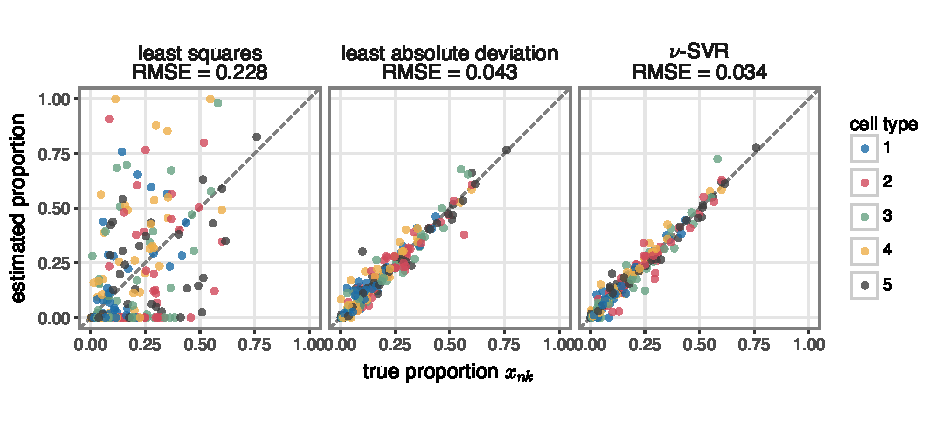
\includegraphics[width=\linewidth]{deconvolution_sim.pdf}
  \caption{Simulated deconvolution. Bulk profiles of $P=400$ genes are mixtures of $K=5$ cell types (immune fraction 30--70\%) plus an unmodelled tumour profile with very high expression of 40 random genes. Estimated against true cell type proportions for least squares, least absolute deviation and $\nu$-SVR, each with negative coefficients set to zero and normalized to sum to one.}
  \label{fig:deconv_sim}
\end{figure}

\subsection{Validation and application}

\citet{newman2015} validated CIBERSORT on blood samples whose composition was measured independently with a Coulter counter, an instrument that counts and sizes cells. The estimated fractions of lymphocytes, monocytes and neutrophils (polymorphonuclear cells, PMNs) correlated with the measured fractions with $R=0.91$ (Figure~\ref{fig:cibersort_validation}). The overall correlation is helped by the large differences between cell types; the agreement within a single cell type, for example the monocytes, is weaker.

\begin{figure}[tbp]
  \centering
  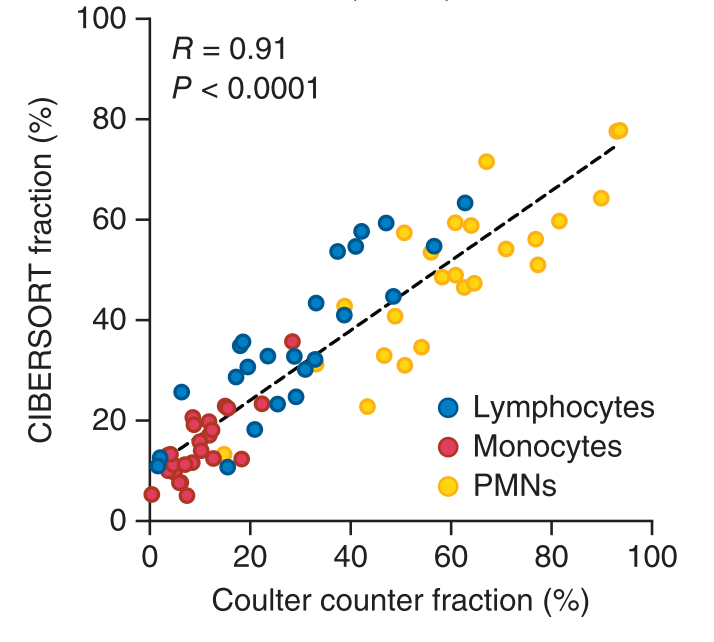
\includegraphics[width=0.45\linewidth]{slides/cibersort_coulter.png}
  \caption{CIBERSORT estimates against Coulter counter measurements of lymphocyte, monocyte and neutrophil (PMN) fractions in blood samples. Reproduced from \citet{newman2015}.}
  \label{fig:cibersort_validation}
\end{figure}

\citet{gentles2015} then applied CIBERSORT to thousands of tumour expression profiles from 25 malignancies with patient survival data. The estimated immune composition differs between cancer types (Figure~\ref{fig:gentles}a). In several blood cancers B cells dominate, because the cancer cells are themselves B cells; brain tumours are rich in monocytes and macrophages. Relating the estimated fractions to survival (Figure~\ref{fig:gentles}b), $\gamma\delta$ T cells were the population most associated with favourable outcomes across cancers, and neutrophils (PMNs) with adverse outcomes. The immune composition of a tumour, estimated computationally from existing bulk data, is thus predictive of prognosis.

\begin{figure}[tbp]
  \centering
  \begin{subfigure}[b]{\linewidth}
    \centering
    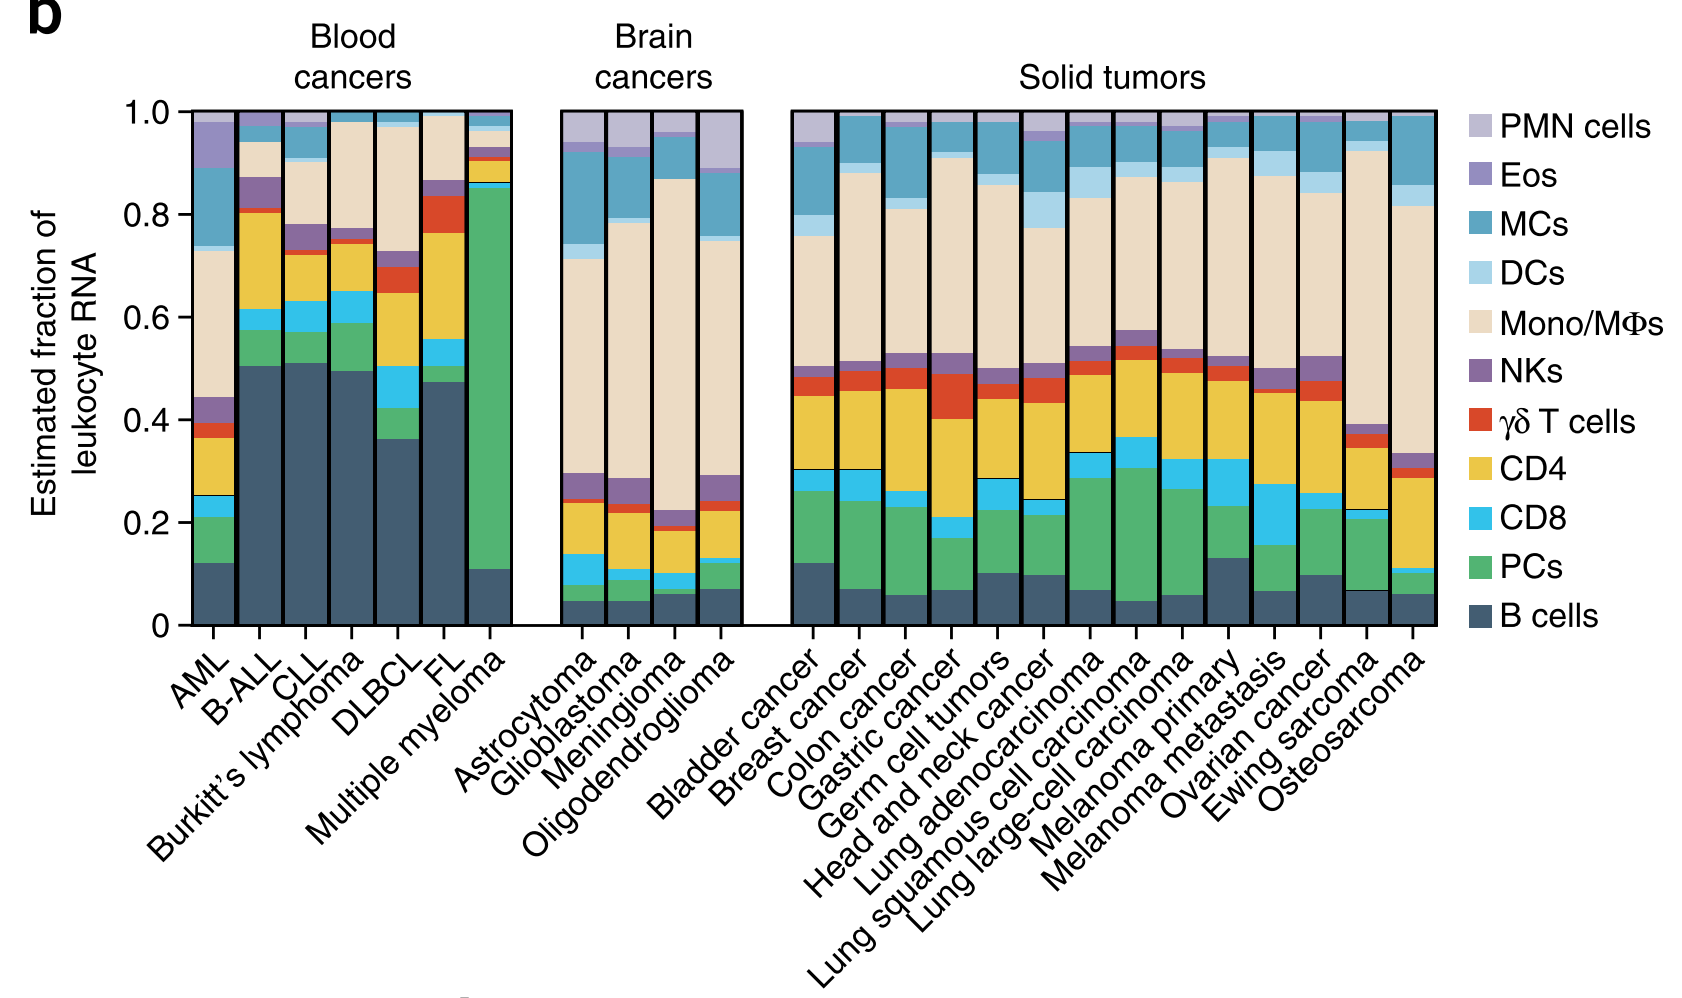
\includegraphics[width=0.85\linewidth]{slides/gentles_fractions.png}
    \caption{}
  \end{subfigure}\\[0.5em]
  \begin{subfigure}[b]{\linewidth}
    \centering
    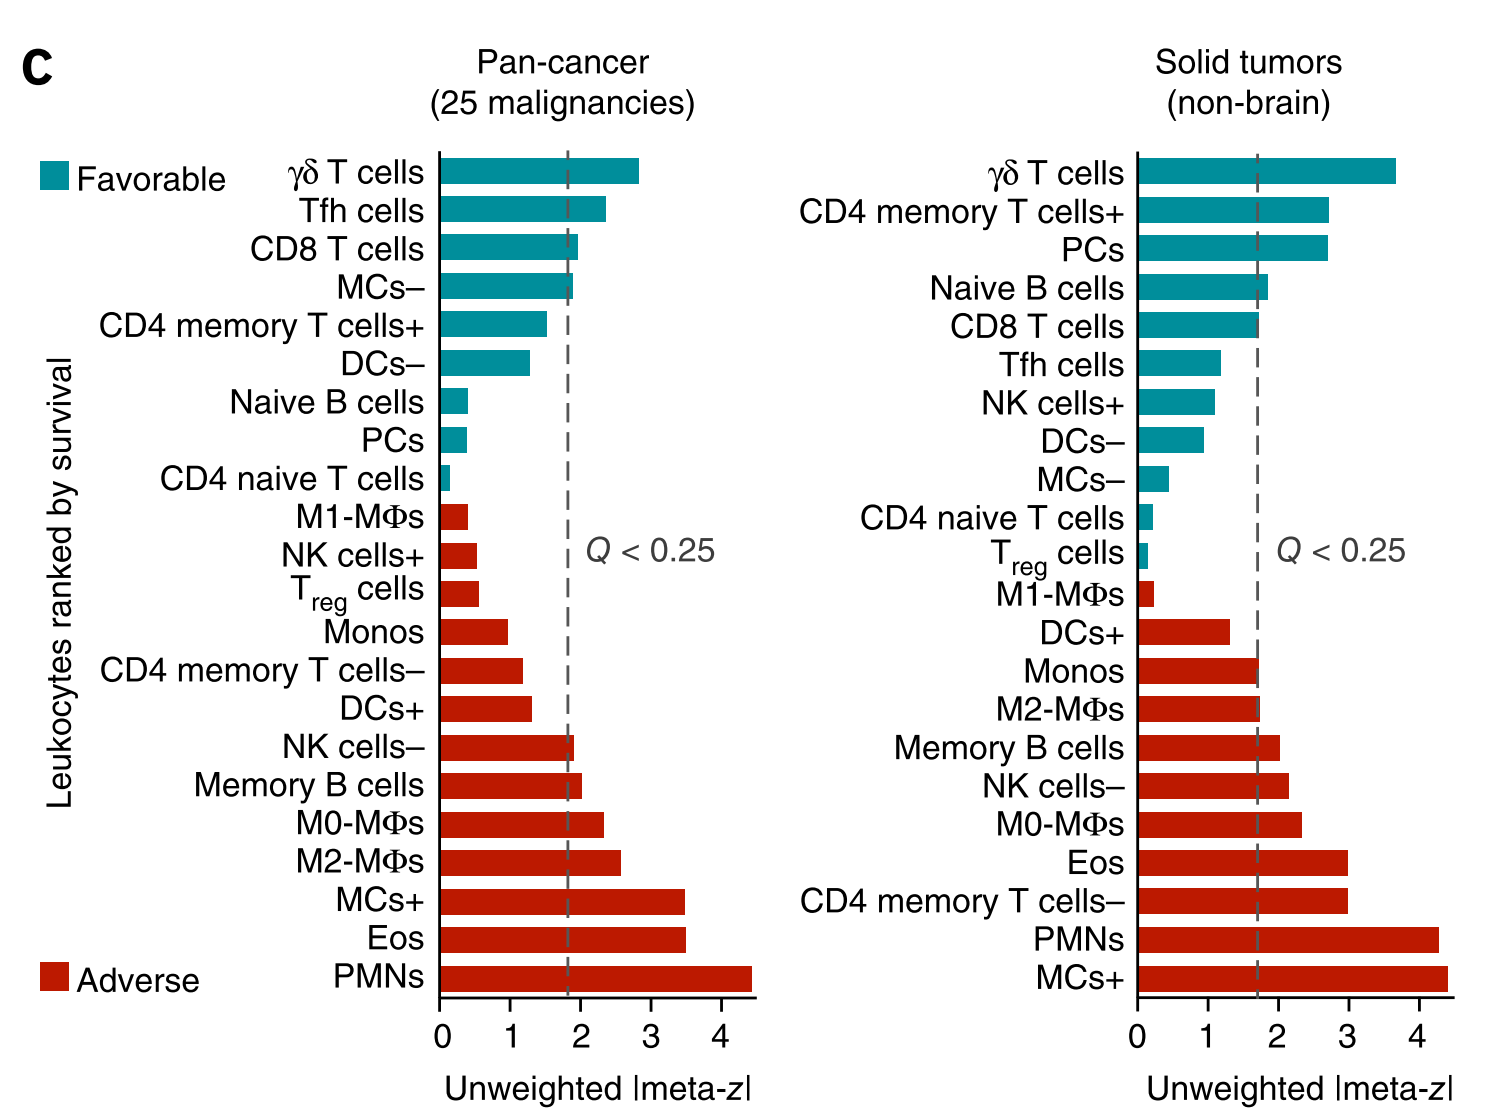
\includegraphics[width=0.75\linewidth]{slides/gentles_survival.png}
    \caption{}
  \end{subfigure}
  \caption{Immune composition of human cancers estimated by CIBERSORT. (a) Estimated fractions of leukocyte RNA by cancer type (panel b of the original). (b) Leukocyte populations ranked by the association of their estimated abundance with survival (meta-analysis $|z|$ score) across 25 malignancies and across non-brain solid tumours; teal, favourable; red, adverse (panel c of the original). MCs, mast cells; PCs, plasma cells; DCs, dendritic cells; M$\Phi$s, macrophages; $+$ and $-$ denote activated and resting states. Reproduced from \citet{gentles2015}.}
  \label{fig:gentles}
\end{figure}

%======================================================================
\section{Summary}
%======================================================================

\begin{itemize}
  \item Matrix factorization models represent each data point as a linear combination of $K$ underlying factors, $\mY\approx\mX\mW^\top$. They are used for dimensionality reduction, visualization, denoising, imputation, removing hidden confounders and integrating datasets.
  \item Factor analysis is the probabilistic base model, with Gaussian factors and feature-specific noise. Integrating out the factors gives a Gaussian with low-rank-plus-diagonal covariance $\mW\mW^\top+\mPsi$, fitted by gradient-based maximum likelihood or by EM. The loadings are identified only up to rotation.
  \item MOFA extends factor analysis to several data types measured on the same samples, with a shared factor matrix and view-specific loadings whose relevance to each view is learned by an ARD prior.
  \item Probabilistic PCA assumes the same noise variance for all features. Its maximum likelihood solution comes from the eigendecomposition of the sample covariance, and PCA is its limit as the noise variance goes to zero. The Marchenko-Pastur law describes the eigenvalues expected from noise and helps choose $K$.
  \item PCA of genotype data reveals population structure, which confounds genetic association studies unless accounted for.
  \item ICA uses heavy-tailed factors, which makes the directions identifiable and suits on-or-off biological programs. NMF constrains both factors to be non-negative and gives parts-based representations; LIGER uses a joint NMF to integrate single-cell datasets.
  \item Autoencoders are the deep learning counterpart; a linear autoencoder learns the PCA subspace.
  \item Cell type deconvolution is a matrix factorization with known loadings. CIBERSORT uses $\nu$-support vector regression, whose robust loss tolerates expression from cell types missing from the signature matrix.
\end{itemize}

%======================================================================
\section*{Exercises}
%======================================================================

\begin{enumerate}
  \item Derive the posterior~\eqref{eq:fa_estep} of the factors in factor analysis from the joint Gaussian distribution of $(\vx_n,\vy_n)$, using the formula for the conditional distribution of a partitioned Gaussian. Show that it agrees with the completing-the-square derivation in the text by using the Woodbury identity.
  \item Implement EM for factor analysis and check that the log likelihood~\eqref{eq:fa_loglik} increases at each iteration. Modify the E- and M-steps to handle missing entries of $\mY$.
  \item Substitute $\hat\mW$ from~\eqref{eq:ppca_ml} into the probabilistic PCA log likelihood and show that the maximizing $\sigma^2$ is the average of the discarded eigenvalues.
  \item Show that the MAP estimate of $\mW$ in probabilistic PCA with the prior $\vw_k\sim\Normal(\vzero,\alpha_k^{-1}\mI)$ on each column, for fixed $\vx_n$, is a ridge regression of $\vy$ on $\vx$. What happens to column $k$ as $\alpha_k\to\infty$?
  \item Verify that the multiplicative update for $\mW$ in NMF is a gradient step with an appropriate element-wise step size, and show that an entry of $\mX$ or $\mW$ that reaches zero stays at zero.
  \item Simulate bulk mixtures as in Figure~\ref{fig:deconv_sim} but without the tumour component. Compare least squares, non-negative least squares and $\nu$-SVR. Which assumption of CIBERSORT does this experiment test, and what changes when a cell type present in the mixture is missing from the signature matrix?
\end{enumerate}

\bibliographystyle{abbrvnat}
\bibliography{chapter08}
\end{document}
